
\documentclass{amsart}
%\usepackage[backend=bibtex8,style=numeric,giveninits=true]{biblatex}
%\addbibresource{formschub.bib}
\usepackage{algorithm}
\usepackage{algpseudocode}
\usepackage{hyperref}
\usepackage{fancyvrb}
\usepackage{amsmath}
\usepackage{amsfonts}
\usepackage{amsthm}
\usepackage{amssymb}
\usepackage{array}
\usepackage{cases}
\usepackage{caption}
\usepackage{xcolor}
\usepackage{tikz}
\usepackage{mathtools}
\usetikzlibrary{calc}
\usepackage{centernot}
\usepackage{mathtools}
\usepackage{graphicx}
\usepackage[margin=1in]{geometry}
\usepackage[makeroom]{cancel}
\usepackage{stmaryrd}
\usepackage{stackengine}
\usepackage{mathrsfs}

%\usepackage{unicode-math}
%\usepackage{nicematrix}

%\usepackage{witharrows}

\newtheorem{lemma}{Lemma}[subsection]
\newtheorem{corollary}[lemma]{Corollary}
\newtheorem{conjecture}[lemma]{Conjecture} 
\newtheorem{proposition}[lemma]{Proposition} 
\newtheorem{theorem}{Theorem}[section]
\newtheorem{observation}{Observation}[section]
\newtheorem{question}{Question}

%\newtheorem{conj}[thm]{Conjecture} 


%%% 
%%% The following gives definition type environments (which only differ
%%% from theorem type invironmants in the choices of fonts).  The
%%% numbering is still tied to the theorem counter.
%%% 

\theoremstyle{definition}
%\newtheorem{definition}{Definition}[section]
%\newtheorem{example}{Example}[section]
\newtheorem{definition}[lemma]{Definition}
\newtheorem{example}[lemma]{Example}
%\newtheorem{algorithm}{Algorithm}
\newtheorem*{note}{Note}

%%
%% Again more of these can be added by uncommenting and editing the
%% following. 
%%

%\newtheorem{note}[thm]{Note}


%%% 
%%% The following gives remark type environments (which only differ
%%% from theorem type invironmants in the choices of fonts).  The
%%% numbering is still tied to the theorem counter.
%%% 


\theoremstyle{remark}

\newtheorem*{remark}{Remark}


%%%
%%% The following, if uncommented, numbers equations within sections.
%%% 

%\numberwithin{equation}{section}
\numberwithin{equation}{subsection}


%%%
%%% The following show how to make definition (also called macros or
%%% abbreviations).  For example to use get a bold face R for use to
%%% name the real numbers the command is $\mathbf{R}.  To save typing we
%%% can abbreviate as

\newcommand{\R}{\mathbf{R}}  % The real numbers.

%%
%% The comment after the defintion is not required, but if you are
%% working with someone they will likely thank you for explaining your
%% definition.  
%%
%% Now add you own definitions:
%%

%%%
%%% Mathematical operators (things like sin and cos which are used as
%%% functions and have slightly different spacing when typeset than
%%% variables are defined as follows:
%%%

\DeclareMathOperator{\sch}{\mathfrak{S}}
\newcommand{\shup}{{\uparrow}}
\newcommand{\downvar}[1]{\stackrel{#1}{\searrow}}
\newcommand{\wof}[1]{w_{#1}}
\newcommand{\rcdd}{\mathfrak{D}}
\newcommand{\wtt}{\mathtt{wt}}
\newcommand{\tom}[1]{\xrightarrow{#1}}
\newcommand{\Tom}[1]{\xRightarrow{#1}}
\newcommand{\mot}[1]{\xleftarrow{#1}}
\newcommand{\cperm}[1]{\llbracket #1\rrbracket}
\newcommand{\cpcf}[5]{d^{#1,#2}_{#3}\left(#4\mid #5\right)}
% simplified product notation
\newcommand{\smpfu}{\mathsf{\Pi}}
\newcommand{\smpr}[3]{\ensuremath{}\smpfu\left( #1 \mid #2_{[#3]}\right)}
\newcommand{\smpre}[2]{\ensuremath{}\smpfu\left( #1 \mid #2\right)}
\newcommand{\rtt}{\mathtt{rt}}
\newcommand{\trm}{\mathtt{trim}}
\newcommand{\zeromap}{\mathcal{Z}}
%\newcommand{\shifthom}{\operatornamewithlimits{\raisebox{1ex}{$\stackrel{\blacktriangleright}{\mathbf{\_}}$}}\limits}

%\newcommand{\shifthom}{\operatornamewithlimits{\raisebox{1ex}{$\blacktriangleright$}}\limits}

\newcommand{\shifthom}{\operatornamewithlimits{\triangleright}\limits}


%\newcommand{\shiftvby}[1]{\ensuremath{\resizebox{\width}{\heightoff}{$\shifthom_{#1}$}}}

\newcommand{\shiftvby}[1]{\shifthom_{#1}}

\newcommand*\circled[1]{%
	\tikz[baseline=(char.base)]{
		\node[shape=circle,draw,inner sep=0.1pt] (char) {#1};
	}%
}
\newcommand\mycircled[1]{\makebox[0pt]{\circled{#1}}}
\newcommand{\tb}{\textbullet}
\newcommand{\xr}[1]{\ensuremath{{}\xrightarrow{[#1]}{}}}
\newcommand{\rd}[1]{\ensuremath{\mathcolor{red}{\mathbf{#1}}}}
\newcommand{\mc}[1]{\ensuremath{\mycircled{#1}}}
\newcommand{\desc}{\mathrm{Desc}}%
%\newcommand{\schv}[2]{\operatornamewithlimits{\sch_{\mathit{#2}}}\limits_{\negphantom{{}_{\mathit{#2}}}\negvphantom{{}_{\mathit{#2}}}#1}}

%\newcommand{\schv}[2]{\setstackgap{S}{0pt}\setstackgap{L}{0pt}\stackMath\stackunder{\sch_{#2}}{\negphantom{\scriptstyle{#2}}\!{\scriptscriptstyle{#1}}}}

\newcommand{\schv}[2]{\shiftvby{#1}\!\sch_{#2}}

%\newcommand{\shiftvby}[1]{\makebox[0pt]{$\triangleright$}#1}



%\newglossary[slg]{symbolslist}{syi}{syg}{List of symbols}
%\makeglossaries

%\begin{itemize}
%	\item Elements of $S_\infty$ $c{[}p,q{]}$, $d{[}p,q{]}$, $r{[}p,q{]}$, homomorphism $\sigma_p:S_\infty\to S_\infty$: Definition \ref{definition:specelem}	

%	\item  Relations between elements of $S\infty$ $\tom{k},\Tom{k}$: Definition \ref{definition:pierisymb}

%	\item Code, dual code, $\code(w)$, $\code^*(w)$, dominant permutations, the dominant approximation $\dom(v)$: Definition \ref{definition:codestuff}

%	\item Function/sets of permutations related to pulling out variables from Schubert polynomials $\varphi_{i,n}$, $\mathcal{D}_i(v)$, $Q_i(v',v)$: Definition \ref{definition:polysequence}

%	\item Flattening function $\phi_i:S_\infty\to S_\infty$, domination relation between permutations: Definition \ref{definition:domination}

%	\item Special polynomials $H_p(x;y)$, $E_p(x;y)$, $\smpr{x_1}{y}{p}$: Definition \ref{definition:hp}

%	\item Polynomial variable omission $x^{(i)}$, subscript substitution $y_A$, index shift function $\shiftvby{i}$: Definition \ref{definition:pv}
%\end{itemize}

\newcommand{\dsch}{\ensuremath{\Xi}}
\newcommand{\coma}{\mathcal{A}}
\newcommand{\dcoma}{\mathcal{D}}



%%
%% This is the end of the preamble.
%% 
\title{The Schubert Algebra and the ring of RC graphs}
\author{Matthew J. Samuel}

%\newcommand{\tomm}[2]{\xrightarrow{#1}_{#2}}
%\counterwithout{equation}{section}
%\setcounter{section}{-1}
\newcommand{\shuff}[2]{\mathcal{S}\mathcal{H}_{#1}^{#2}}
\newcommand{\dom}{\mathfrak{d}}
\newcommand{\ldom}{\dom^*}
\newcommand{\code}{\mathfrak{c}}
\newcommand{\ducode}{\overline{\mathfrak{c}}}

\newcommand{\maxd}{\mathfrak{m}}
\newcommand{\ddv}[1]{{{}_{{\scriptscriptstyle (#1)}}\partial}}
%\newglossary[slg]{symbolslist}{syi}{syg}{Symbolslist}
%\GlsXtrLoadResources
%[src={symbols},sort=use,type=main,
%	group=specelem]
%\glsaddstoragekey{group}{}{\grouplabel}
%\glsxtrsetgrouptitle{specelem}{}





%\newglossary[slg]{symbol}{sot}{stn}{Symbols}
%\makeglossaries

\begin{document}
	\maketitle
	
\section{Some preliminaries}
\subsection{Notation}
\begin{definition} \label{definition:polysequence}
		For a permutation $v'$ such that $v'\in S_{n}$, define
		$$\varphi_{i,n}(v')(j)=\begin{cases}
			v'(j)&\mbox{ if }j<i\\
			n+1&\mbox{ if }j=i\\
			v'(j-1)&\mbox{ if }i<j\leq n+1\\
			j&\mbox{ if }j>n+1
		\end{cases}$$
		Now fix $v\in S_n$ and $i\geq 1$ an integer, we define a relation $\downvar{i}$ by declaring that $v\downvar{i} v'$ if 
		$$v\Tom{i}\varphi_{i,n}(v')$$
		Equivalently, $v\downvar{i} v'$ if whenever $v\in S_n$ and $n$ is minimal, we have that $v$ satisfies the relation $\Tom{i}$ with respect to the permutation obtained from $v'$ by inserting $n+1$ at position $i$. We note that this concept was introduced by Bergeron and Sottile in \cite{bsskew}.
		
		If $v\downvar{i} v'$, we define a set of integers $Q_i(v',v)$ by
		$$Q_i(v',v)=\{v(j)\mid j>i\mbox{ and }v'(j-1)=v(j)\}$$
		Given the fact that any element of $S_\infty$ fixes all but finitely many positive integers, it follows that $Q_i(v',v)$ is a finite set.
		
		We then define $\mathcal{D}_i(v)$ to be all permutations $v'\in S_\infty$ such that $v\downvar{i} v'$. The permutations $\mathcal{D}_i(v)$ arise when pulling a variable out of a Schubert polynomial and expressing the coefficients of the powers of this variable as Schubert polynomials in the remaining variables, as is done in \cite{coprod}, from which this definition essentially comes.

		For a permutation $v\in S_\infty$, we define $\shup{v}$ to be the permutation defined by
		$$\shup{v}(i) = \begin{cases}
			v(i-1)+1&\mbox{ if }i>1\\
			1&\mbox{ if }i=1
		\end{cases}$$
		Recursively, we define $\shup^k(v)$ to be $\shup(\shup^{k-1}(v))$.

		For a permutation $w$, we define $\maxd(w)$ to be the maximum right descent of $w$. That is
		$$\maxd(w) = \max\{i\mid w(i)>w(i+1)\}$$

		Define
		$$\smpre{a}{B} = \prod_{b\in B}(a-b)$$
	\end{definition}

	\begin{proposition}[Special case of Pieri formula {\cite[Theorem~7.1]{samuelmolev}}] \label{proposition:pieri}
Suppose $k\geq 1$ and $u,w\in S_\infty$. If $u\not\tom{k} w$, then
$$\ddv{y}_u^w\smpr{x_1}{y}{k}=0$$
If $u\tom{k} w$, define
$$Q = \{u(i)\mid i\leq k\mbox{ and }u(i)=w(i)\}$$
then
$$\ddv{y}_u^w\smpr{x_1}{y}{k}=\smpre{x_1}{y_Q}$$
\end{proposition}
\begin{proof}
	This is simply a change of variables from the original theorem.
\end{proof}

The next proposition specializes, in the case of ordinary Schubert polynomial $\sch_v(x)$, to a formular that isolate a chosen index $i$: one can express $\sch_v(x)$ as a sum of terms of the form $x_i^p\sch_{v'}(x^{(i)})$, thereby effectively extracting the variable $x_i$ and leaving Schubert polynomials in the remaining variables \cite[Theorem~5.1]{bsskew}. Proposition \ref{proposition:pullindex} is the double Schubert polynomial version of this, which, as far as we know, is new.% A more general formula is possible for arbitrary splitting into disjoint sets of indices, similar to the formula in \cite{bsskew} and using the same method of proof as Proposition \ref{proposition:pullindex} coupled with the main result of \cite{samuelleibniz}, though we will not need this here.


\begin{proposition} \label{proposition:pullindex}
Let $v\in S_\infty$ and let $i>0$ be an integer. Then we have
$$\sch_v(x;y)=\sum_{v\downvar{i} v'}\smpre{x_i}{y_{Q_i(v',v)}}\sch_{v'}(x^{(i)};y)$$
\end{proposition}
\begin{proof}
Suppose $v\in S_n$. We have
$$\sch_v(x;y)=\ddv{y}^{vw_0(n)}(\sch_{w_0(n)}(x;y))$$
This is equal to
$$\ddv{y}^{vw_0(n)}(\sch_{s_{n+1-i}\cdots s_1w_0(n)}(x^{(i)};y)\smpr{x_i}{y}{n+1-i})$$
and, applying the Leibniz formula, is also equal to
$$\sum_{\substack{v'\in S_\infty\\\ell(v'w_0(n)s_1\cdots s_{n+1-i})=\ell(w_0(n)s_1\cdots s_{n+1-i})-\ell(v')}}\sch_{v'}(x^{(i)};y)\ddv{y}_{v'w_0(n)s_1\cdots s_{n+1-i}}^{vw_0(n)}\smpr{x_i}{y}{n+1-i}$$
By the restricted Pieri formula (Proposition \ref{proposition:pieri}), for this to be nonzero necessarily $v'w_0(n)s_1\cdots s_{n+1-i}\tom{n+1-i}vw_0(n)$. We note that $v'w_0(n)s_1\cdots s_{n+1-i}\tom{n+1-i}vw_0(n)$ if and only if 
$$v\Tom{i}v'w_0(n)s_1\cdots s_{n+1-i}w_0(n)=v's_ns_{n-1}\cdots s_i$$
We have that $v's_n\cdots s_i$ is exactly $\varphi_{i,n}(v')$ since $v'\in S_n$, so we require that
$$v\Tom{i}\varphi_{i,n}(v')$$
so the sum is over all $v'\in \mathcal{D}_i(v)$.

Applying Proposition \ref{proposition:pieri}, we obtain that the result is equal to
$$\sum_{v'\in \mathcal{D}_i(v)} \smpre{x_i}{y_{A(v',v)}}\sch_{v'}(x^{(i)};y)$$
where $A(v',v)$ is the set of all $vw_0(n)(j)$ such that $1\leq j\leq n+1-i$ and $v'w_0(n)s_1\cdots s_{n+1-i}(j)=vw_0(n)(j)$. These values are the same as at the indices that comprise the set of all $1\leq j\leq n+1-i$ such that
$$v'(n+2-s_1\cdots s_{n+1-i}(j))=v(n+2-j)$$
Applying the $s_1\cdots s_{n+1-i}$ to $j$, since $1\leq j\leq n+1-i$ we have that 
$$s_1\cdots s_{n+1-i}(j)=j+1$$
Hence we need
$$v'(n+2-(j+1))=v'(n+1-j)=v(n+2-j)$$
Replacing $j$ with $n+2-p$, the indices are the set of all $p$ such that $i<p\leq n+1$ and
$$v'(p-1)=v(p)$$
Thus $A(v',v)$ is the set of all $v(p)$ such that $p>i$ and $v'(p-1)=v(p)$, which is exactly $Q_i(v',v)$, and we are done.
\end{proof}


\section{The Schubert Algebra and its dual}

\subsection{Definition}


We define a commutative algebra $\coma$ over the integers as follows. For each $n$, define $\coma_n$ to be the polynomial ring over $\mathbb{Z}$ in the variables $x_1,\ldots,x_n$. Then define
$$\coma =\bigoplus_{n=0}^\infty \coma_n$$
The multiplication within $\coma_n$ is as usually defined for the polynomial ring. However, if $a\in \coma_m$ and $b\in \coma_n$ with $m\neq n$ and $m,n>0$,  then
$$ab = 0$$
Otherwise, the component for $n=0$ is identified with the coefficient ring. Note that the ``identity element'' for positive $n$ is not an identity element of $\coma$ (we may sometimes refer to it as a ``fat identity'').

Each $\coma_n$ has a basis consisting of elements $x_a^{(n)}$, where $a$ is a sequence of $n$ nonnegative integers, and the notation indicates that
$$x_a = x_1^{a_1}\cdots x_n^{a_n}$$
The direct sum therefore has a basis that can canonically be identified with union of these.

We define a coproduct $\Delta:\coma\to\coma\otimes\coma$ on the basis $x_c^{(n)}$ by
$$\Delta(x_c^{(n)}) = \sum_{\substack{p+q=n\\ab=c}} x_a^{(p)}\otimes x_b^{(q)}$$
where the equation $ab=c$ indicates that $a$ concatenated with $b$ is equal to $c$. We also define a counit $\varepsilon:\coma\to \mathbb{Z}$ by $\varepsilon(x_a^{(n)})=0$ unless $n=0$.

\begin{lemma}
	With $\Delta$ and $\varepsilon$, $\coma$ is a coassociative, counital coalegebra.
\end{lemma}
\begin{proof}
	We have 
	$$\Delta(x_d^{(n)})=\sum x_a^{(p)}\otimes x_c^{(q)}$$
	Applying $\Delta$ to either tensor factor results in
	$$\sum x_a^{(p)}\otimes x_b^{(q)}\otimes x_c^{(r)}$$
	The symmetry of this is exactly the coassociativity condition. Seeing that we may choose $p=n$ or $q=n$, the definition of the counit gives us the result that $\coma$ is counital as well under $\Delta$ and $\varepsilon$.
\end{proof}

\begin{lemma}
	$\Delta:\coma\to\coma\otimes\coma$ is a homomorphism of rings.
\end{lemma}
\begin{proof}
	This is where the condition that $x_a^{(p)}x_b^{(q)}=0$ unless $p=q$ when both $p,q>0$ comes in. It ensures that only monomials of the same length have nonzero products and preserves the structure of the coproduct as a homomorphism of rings.
\end{proof}

\begin{lemma}
	$\nabla:\coma\otimes \coma\to \coma$ is a homomorphism of coalgebras.
\end{lemma}
\begin{proof}
	
\end{proof}

\begin{corollary}
	$\coma$ is a bialgebra over $\mathbb{Z}$.
\end{corollary}

$\coma$ is afforded a grading into finite dimensional components by observing that each $\coma_n$ itself is a graded ring with each homogeneous component being a finitely generated free module. Considering the pair $(n, d)$, where $n$ is the number of variables and $d$ is the degree, as a $\mathbb{Z}^2$ grading, we may take the graded dual module $\dcoma$, which, by virtue of the grading, is isomorphic as a free module to $\coma$. We identify the dual basis element $x_a^*$ with the sequence of nonnegative integers $a$. That is to say,
$$\langle a, x_b\rangle = \delta_{ab}$$
Inspection of the coproduct reveals that the product of $a$ and $b$ in $\dcoma$ is simply the concatenation $ab$. Hence $\dcoma$ is isomorphic to the free associative algebra on a countable set indexed by nonnegative integers.

$\dcoma$ also has a coproduct compatible with its product, namely
$$c\mapsto \sum_{a+b=c} a\otimes b$$
Thus $\coma$ and $\dcoma$ are dual bialgebras.

Calling $\coma$ the ``Schubert algebra'' may seem unnecessarily grandiose, however the reason will become clear below.

\subsection{The Schubert basis}

In $\coma$, each $\coma_n$ has a basis of Schubert polynomials $\sch_u^{(n)}$, where the largest right descent of $u$ is at most $n$, ensuring that $\sch_u(x)$ has at most $n$ variables. Schubert polynomials limited to a specific number of variables have well-defined structure constants $c_{u,v}^w$, independent of $n$, given by
$$\sch_u^{(n)}\sch_v^{(n)} = \sum_{w}c_{u,v}^w\sch_w^{(n)}$$
These are known to be nonnegative integers, however except in special cases no positive combinatorial formula is known.

Schubert polynomials have nonnegative coefficients in terms of the $x_a^{(n)}$ basis, for which many formulas are known. There is also a less well-understood unique expansion of the Schubert polynomials into sums of products of elementary symmetric polynomials with at most $n$ variables. %For a fixed positive integer $n$ define the \emph{classical elementary monomials} of rank $n$ to be products of the form
%$$e_{i_1}^{\lambda_1}\cdots e_{i_p}^{\lambda_p}$$
%where $\lambda$ is a conjugate of a strict partition of length exactly $n$.


\newcommand{\sdom}{\widetilde{\mu}}

%For a permutation $u$ with the last descent of $u$ at most $m$, define a strict partition $\sdom_m(u)$ as follows. If $\code(u)$ is a strict partition of length exactly $m$, define $\sdom_m(u)=u$.  Otherwise, let $i<m$ be the maximal index with $\code_i(u)\leq \code_{i+1}(u)$, and define $\sdom_m(u) = \sdom_m(us_i)$. Then define
%$$\sdom_m^*(u) = \sdom_m(u^{-1})^{-1}$$

%\begin{lemma}
%Suppose $\sch_u(x)$ has at most $p$ variables. Then for each $m\geq p$ there are unique coefficients $E_{u,a}^{\lambda_m}$ with $a_i\leq \lambda_m(u)$ for all $i$, where $\lambda_m(u)$ is the conjugate of a strict partition of length exactly $m$, such that
%$$\sch_u^{(m)} = \sum_{a} E_{u,a}^{\lambda_m}e_a^{\lambda_m}$$
%\end{lemma}

\subsection{The elementary basis}

%Define an $n$-elementary partition to be a partition $\lambda$ such that $\lambda_1\leq n$, and if $\lambda_i<n$ then either $\lambda_{i-1}=\lambda_i=0$ or $\lambda_{i-1} = \lambda_i + 1$. For an $n$-elementary partition $\lambda$, we define $\epsilon_n(\lambda)$ to be the last index such that $\lambda_{\epsilon_n(\lambda)}=n$. 
We say that a weak composition $\alpha$ is \emph{$n$-elementary} if $\alpha_i\leq i$ for all $i\leq n$ and $\alpha_i\leq n$ for all $i>n$, satisfying the additional restriction that $\alpha_i\geq \alpha_{i+1}$ if $i\geq n$.

An $n$-elementary monomial is a an element of the polynomial ring of the following form: 
$$e_{\alpha_1}^{1}\cdots e_{\alpha_n}^ne_{\alpha_{n+1}}^n\cdots e_{\alpha_m}^n$$
where $\alpha$ is an $n$-elementary weak composition. Define $\mathcal{E}_n$ to be the set of $n$-elementary monomials.

\begin{theorem}
	$\mathcal{E}_n$ forms a $\mathbb{Z}$-basis for $\coma_n$, and $\bigcup_{n}\mathcal{E}_n$ forms a basis for $\coma$.
\end{theorem}
\begin{proof}
	It is a theorem of Macdonald that the polynomial ring $\mathbb{Z}[x_1,\ldots,x_n]$ is a free module over $\Lambda_n$ with basis the Schubert polynomials $\sch_u(x)$ such that $u\in S_n$. These Schubert polynomials are uniquely expressed in terms of strict elementary symmetric monomials with fewer than $n$ variables. Since $\Lambda_n$ is a polynomial ring in the $e_{i,n}$ by the fundamental theorem of elementary symmetric polynomials, $\Lambda_n$ has a basis of monomials $e_{\lambda,n}$ as $\lambda$ ranges over all partitions with parts bounded by $n$. The multiplicative combination of these two bases is therefore a $\mathbb{Z}$-basis of $\coma_n$. This is exactly the description of the monomials $e_{\alpha}^n$ for $\alpha$ an $n$-elementary weak composition.
\end{proof}

We can ask for transition formulas between the Schubert and the elementary basis. From elementary to Schubert, we may use Sottile's Pieri formula. That is,

$$e_{\alpha}^n = \sum_{1\xrightarrow{1,2,\ldots,n}_{\alpha} u}\sch_u^n$$

For the reverse transition, suppose we want to express $\sch_w^n$ in the elementary basis. Let $\lambda = \mu^*_n(w)$ and consider the double Schubert polynomial
$$\sch_{\lambda}(x;y)=\prod_i E_{\lambda_i}(x;y_i)$$
We have that
$$\sch_w(x;y) = \partial_y^{w\lambda^{-1}}\sch_\lambda(x;y)$$
Applying the Leibniz formula, this is
$$\sum_{u_0\xrightarrow{1} u_1\cdots}\prod_i \partial^{u_i/u_{i-1}}_yE_{\lambda_i}(x;y_i)$$
It is possible to find a combinatorial formula for each factor in the product, keeping the $y$ variables, but we only need the sign. We define $\sigma_i(u_{i-1},u_i)$ to be the number of indexes $j<i$ such that $u_{i-1}(j)\neq u_i(j)$. Then we define
$$\sigma(P)=\sum_i \sigma_i(u_{i-1},u_i)$$
%$$\sch_w^n = \sum_{P:1\xrightarrow{\lambda} w\lambda^{-1}} (-1)^{|\lambda| - \ell(w) + \sigma(P)}e_{\alpha(P,\lambda),\lambda}^n$$
Then we define
$$E^{\alpha;n}_w = \sum_{\substack{P:1\xrightarrow{1,2,\ldots,n} w\lambda^{-1}\\\alpha(P)=\alpha}}(-1)^{|\lambda|-\ell(w)+\sigma(P)}$$

\begin{theorem}
	For each $w$, we have
	$$\sch_w^n = \sum_{\alpha}E_w^{\alpha}e_{\alpha}^n$$
\end{theorem}
These numbers are stable for fixed $w$ as soon as the number of variables is at least as large as the value of $n$ such that $w\in S_n$, and are well-studied but poorly understood.

\begin{example}
	Let $n=5$ and let $w$ be the permutation such that $\code(w)=(0,2,0,2,3)$. Let $\lambda = (5,5,5,4,3,2,1)$. Then
	\begin{align*}
		\sch_w^n &= e_{(0,0,0,0,5,1,1)} - e_{(0,0,0,0,4,2,1)} + e_{(0,0,0,0,4,3)}- e_{(0,1,0,0,4,1,1)} +e_{(0,0,1,0,3,2,1)}\\
		&+e_{(0,1,0,0,5,1)} + e_{(0,1,0,0,3,3)}
	\end{align*}
\end{example}
%\section{The Schur-elementary basis}

%$\Sigma_n$
%$$c_{u,\lambda^{\perp,m}}^{w\mu_{n,m}w_0(n-1)}E_{u,a}^ns_{\lambda}(x_1,\ldots,x_n)e_{a}$$

%Express $w_0(n,m)$ as $\sch_{w_(n-1)}(x)E_n(x)^m$.

% e_3e_3e_2e_1
Suppose $\alpha$ and $\beta$ are weak compositions. We define $\alpha\|_p \beta$ to be the weak composition defined by
$$\gamma_i = \begin{cases}
	\alpha_i&\mbox{ if }i\leq p\\
	\alpha_i + \beta_{i-p}&\mbox{ if }i> p
\end{cases}$$

\begin{theorem}
	$$\Delta(e_\gamma^n) = \sum_{\substack{\alpha \|_p \beta=\gamma\\p+q=n}} e_{\alpha^{\overline{p}}}^p\otimes e_\beta^q$$
	where $\alpha$ ranges over all weak compositions such that $\alpha^{\overline{p}}$ is $p$-elementary and $\beta$ ranges over all $q$-elementary weak compositions.
\end{theorem}

\subsection{The Schubert-Schur and separated descents basis}

%Schur-Schubert structure constants are positive, and the Schubert basis is positive in the Schur-Schubert basis.

$\coma_n$ has a basis of the form $S_{\lambda,u}^n=s_\lambda(x_1,\ldots,x_n)\sch_u(x)$, where $u\in S_n$ and $s_\lambda$ is the Schur polynomial corresponding to $\lambda$ in $\Lambda_n$. This is called the \emph{Schubert-Schur} basis. There is a generalization that this is an easy special case of that can be described as follows.
%$$S_{\lambda,u}^n = \sum c_{v_{\lambda;n},u}^{w}\sch_w^n$$

%Thus

%$$\dsch_w^n = c_{v_{\lambda;n},u}^w\Omega_{\lambda,u}^n$$

%\section{The separated descents basis}

Let $K_{u,v;k}^n = \sch_u(x_1,\ldots,x_n)\sch_v(x_1,\ldots,x_{k-1})$, where $v\in S_k$ and $u$ is a permutation such that $\ell(us_i)>\ell(u)$ for all $i<k$. We will call this the \emph{separated descents basis} for the descent $k$.

\begin{theorem}
	For fixed $k$, $K_{u,v;k}^n$ form a basis of $\coma_n$ for all $n\geq k$.
\end{theorem}
\begin{proof}
	First we show that these elements additively generate the subring. Note first that $\mathcal{E}_n$ is a basis. Let $e_{\alpha_1}^{\lambda_1}\cdots e_{\alpha_m}^{\lambda_m}\in \mathcal{E}_n$. Let $j$ be the index such that $\lambda_j=k$. Let
	$$P=\prod_{i=1}^j e_{\alpha_i}^{\lambda_i}$$
	and let
	$$Q=\prod_{i=j+1}^{m} e_{\alpha_i}^{\lambda_i}$$
	By the fact that $\lambda_{i-1} = \lambda_i +1$ for all $i>j$, it follows that
	$$Q=\sum c_v\sch_{v}(x)$$
	for integers $c_v$ with $v\in S_k$. Given the fact that $P$ is symmetric in $x_1,\ldots,x_k$, it can be shown that
	$$P=\sum d_u\sch_u(x)$$
	for integers $d_u$ and permutations $u\in S_\infty$ with $\ell(us_i)>\ell(u)$ for all $i<k$. Thus the $n$-elementary monomial can be expressed as
	$$PQ=\sum c_ud_v\sch_u(x_1,\ldots,x_n)\sch_v(x_1,\ldots,x_{k-1})$$
	Since the $n$-elementary monomials form a basis, this proves that $K_{u,v;k}^n$ spans $\coma_n$.
	
	To prove independence, first note that if 
	$$\sum_{u} c_{u}K_{u,1;k}^n = \sum_u c_u\sch_u(x)= 0$$
	then $c_u=0$ for all $u$ by independence of Schubert polynomials. Assume the inductive hypothesis that for some $m>0$ we have that if 
	$$\sum_u c_{uv}K_{u,v;k}^n=0$$ 
	and for all $v$ in the sum with $\ell(v)\geq m$ we have $c_{uv}=0$, then $c_{uv}=0$ for all $u$ and $v$. For a sum with possibly nonzero terms such that $\ell(v)=m$ at most, suppose
	$$\sum_{u,v} c_{u,v}K_{u,v;k}^n = 0$$
	Let $i$ be a positive integer. Then by applying the divided difference $\partial^{s_i}$ we see that
	$$\sum_{u,v} c_{u,v}K_{u,vs_i;k}^n = 0$$
	for all $v$ with $\ell(vs_i)<\ell(v)$. In particular, the maximum length with a possibly nonzero coefficient has decreased by at least $1$. By the inductive hypothesis, all terms in this sum are $0$, hence $c_{uv}=0$ for all $u$ and $v$ with $\ell(vs_i) < \ell(v)$. Iterating over all $i$, we have the result.
\end{proof}

For transition coefficients, expressing $K_{u,v;k}^n$ in terms of Schubert polynomials is ``easy'' and combinatorially known to have nonnegative coefficients. While positive formulas are known, their discovery is quite recent.

Expressing the Schubert basis in terms of $K_{u,v;k}^n$ can be done as follows.

Recall we can express $\sch_w^n$ as
$$\sch_w^n = \sum_{\alpha} E_w^{\alpha;n}e_{\alpha}^n$$
To transition to the basis $K_{u,v;k}^n$, let $a$ be the index such that $\lambda_a = k$. Then
$$\sch_w^n = \sum_{\alpha} E_w^{\alpha;n}\left(\prod_{i=1}^a e_{\alpha_i,\lambda_i}\right)\left(\prod_{j=a+1}^{\ell(\lambda)} e_{\alpha_j,\lambda_j}\right)$$
These products can be expanded with the Pieri formula as
$$\sch_w^n = \sum_{\alpha}E_w^{\alpha;n}c_{\alpha',\lambda'}^uc_{\alpha'',\lambda''}^vK_{u,v;k}^n$$

\begin{example}
	Let $n=5$, let $k=3$, and let $w$ be the permutation such that $\code(w)=(0,2,0,2,3)$. Then
	$$\sch_w^n =K_{12468357, 132;3}^5 - K_{13468257, 1; 3}^5$$
	If instead we let $k=4$, we obtain
	$$\sch_w^n =-K_{124563, 132;4}^5+ K_{1246735, 132;4}^5+ K_{134562, 1;4}^5- K_{1346725, 1;4}^5+ K_{234561, 132;4}^5$$
\end{example}


%\section{Skew dual Schubert elements}

%Positive for $n-3$-separated for $u$ $(n-3, n-2, n-1)$-step.


%$$\dsch_w^n = \sum c_{u,v}^wO_{u,v;k}^n$$

%Change to the numvars sepdesc basis

%$$\dsch_{w/u}^n = c_{u',v'}^wc_{u,v}^{v'}O_{u',v';k}^n$$


%$$\dsch_{w/u}^n = c_{u,v'}^wc_{u',v}^{v'}O_{u',v';k}^n$$




%asbg
%$$\dsch_{w/u}^n = c_{u,u',v'}^wO_{u',v';k}^n$$

%$$\dsch_{w/u}^n = c_{u,u'}^{v}c_{v,v'}^wO_{u',v';k}^n$$

%$$\dsch_{w/u}^n = c_{u,u'}^{v}c_{v,v'}^wO_{u',v';k}^n$$

%$u$ is $k$-symmetric, positive

%Positive in the Schur-elementary basis

%Monomial symmetric function

%Schubert-Schur has an associative duality

%Grassmannian basis?

%Separated descents basis

%There is a basis $O_{u,v;k}^n$ where $v\in S_k$ and $u$ has no descents less than $k$.
%Just the coproduct of $w\mu^{-1}$

%Schubert-Schur $k$ times Schubert is positive separated descents $k$.

%$\Omega_{\lambda,u}^p\dsch_v^q$ is positive in $O_{u',v';p}^{p+q}$.

%Adjoint of the coproduct

%$$\langle \dsch_v^q, d_{u,v'}^w(p,q)\sch_{v'}^q\rangle$$

%	$$\langle \dsch_v^q, \sch_{w/u}^q(p)\rangle$$

%In this basis, we claim $s_\lambda\sch_u\mapsto s_{\lambda^\perp}\sch_{w_0uw_0}$ is an involutory automorphism of rings.

%$$\Omega_{\lambda,u}^p\Omega_{\mu,v}^q = c_{\lambda,\mu}^{\nu}d_{u,v}^w(p,q)\Omega_{\nu,w}^{p+q}$$
%\section{The Schur-Artin basis}

%\section{The descending Schur basis (Schur-elementary)}


\subsection{The dual algebra}

We examine the graded dual algebra $\dcoma$ more closely now. This is a graded ring generated by countably many elements that we denote by $[i]$, where $i$ is a nonnegative integer. The product, as mentioned previously, is concatenation of sequences. Thus
$$[a_1\cdots a_p][b_1\cdots b_q]=[a_1\cdots a_pb_1\cdots b_q]$$
It is not hard to see that $\dcoma$ is a free algebra on these generators. Thus the set of sequences $[a_1\cdots a_n]$ forms a $\mathbb{Z}$-basis for $\dcoma$. We may realize this as the dual of $\coma$ by declaring that
$$\langle [a_1\cdots a_n],x_1^{b_1}\cdots x_n^{b_n}\rangle = \prod_i\delta_{a_i,b_i}$$

We have a $\mathbb{Z}\times \mathbb{Z}$ grading such that
$$\deg([a_1\cdots a_n])=(n,-a_1-a_2\cdots-a_n)$$
The set of elements such that $\deg(a) = (n,-)$ is $\dcoma_n$, dual as a graded module to $\coma_n$.

\subsection{The dual Schubert basis}
       
There is a basis $\dsch_u^{n}$ dual to the Schubert basis for $\dcoma_n$. Specifically, with the unique pairing $\langle -,-\rangle:\dcoma\times \coma\to\mathbb{Z}$ such that
$$\langle \alpha,x_\beta\rangle = \delta_{\alpha\beta}$$
we define $\dsch_u^n$ to be the unique basis of $\dcoma_n$ such that
$$\langle \dsch_u^n,\sch_v^n\rangle = \delta_{uv}$$
We characterize it with an explicit formula.

\begin{theorem}
	For each permutation $u$ and integer $n$ with $\ell(us_i)>\ell(u)$ for all $i>n$ we have the equation
	$$\dsch_u^{n} = \sum_{\ell(\alpha)=n} E^{\code(\mu)-\alpha,\code(\mu)}_{u\mu^{-1}}\alpha$$
	where $\mu$ is any strict dominant permutation such that $0\neq \code_n(\mu) \geq \ell(u)$ and $\code_{n+1}(\mu)=0$.
\end{theorem}
\begin{proof}
	By definition, the coefficient of $\alpha$ in $\dsch_u^n$ is the coefficient of $\sch_u^n$ in $x_\alpha$. This can be derived from the Cauchy formula for double Schubert polynomials. Note that for any permutation $\mu$ as laid out in the statement of the theorem, $\ell(u\mu^{-1})=\ell(\mu)-\ell(u)$. Thus,
	$$\partial_y^{u\mu^{-1}}\sch_\mu(x;-y) = \sch_u(x;-y)$$
	We have that
	$$\sch_\mu(x;-y)=\sum_u \sch_u(x)\sch_{u\mu^{-1}}(y)$$
	Expressing the second factor in the $e_{\alpha,\lambda}(y)$ basis, we have
	$$\sch_\mu(x;-y)=\sum_{u,\alpha} \sch_u(x)E_{u\mu^{-1}}^{\code(\mu)-\alpha,\code(\mu)}e_{\code(\mu)-\alpha,\code(\mu)}(y)$$
	An alternative expression for $\sch_\mu(x;-y)$ is
	$$\sch_\mu(x;-y)=\sum_{\alpha} x_\alpha e_{\code(\mu)-\alpha,\code(\mu)}(y)$$
	from which we see that the coefficient is correct.
\end{proof}

This is not stable for fixed $u$ as $n$ increases, and this is expected.


\begin{lemma}
	Let $u,v\in S_\infty$ and $p,q>0$ be integers. Write
	$$\dsch_u^p\dsch_v^q = \sum_w d_{u,v}^w(p,q)\dsch_w^{p+q}$$
	Then for each $u,v,w$ the coefficient $d_{u,v}^w(p,q)$ is the coefficient of $\sch_u(x_1,\ldots,x_p)\sch_v(x_{p+1},\ldots,x_{p+q})$ in the expansion of $\sch_w(x_1,\ldots,x_{p+q})$ in terms of the basis of products of Schubert polynomials in $x_1,\ldots,x_p$ and Schubert polynomials in $x_{p+1}$ onward.
\end{lemma}
\begin{proof}
	This is true by examination of the definition of the coproduct of $\coma$, since this is the coefficient of $\sch_u^p\otimes \sch_v^q$ in the coproduct of $\sch_w^{p+q}$.
\end{proof}

Thus the product structure of $\dcoma$ encodes splitting of the Schubert polynomial into two sets of variables. In particular,
\begin{lemma} \label{lemma:dpieri}
Let $a\geq 0$ be an integer and $w\in S_\infty$. Then we have
$$[a]\cdot \dsch_{w}^{n} = \sum_{\substack{w\in\mathcal{D}_1(w')\\\ell(w,w')=a}} \dsch_{w'}^{n+1}$$
\end{lemma}

% Due to the fact that we have a positive formula for the coproduct of $\coma$, we have a Littlewood-Richardson rule for $\dcoma$ in the Schubert basis.
% \begin{theorem}[Littlewood-Richardson rule for $\dcoma$]
% 	We have
% 	$$\dsch_u^{p}\dsch_v^{q} = \sum_w c_{uw_0(p+q)w_0(q),vw_0(q)}^{ww_0(p+q)}\dsch_w^{p+q}$$
% 	where $c_{u',v'}^{w'}$ indicates the usual Schubert structure constants. In particular, we have a positive formula for these structure constants.
% \end{theorem}

% We also have the following Pieri formula.

% \begin{theorem} \label{theorem:pieri}
% 	Let $a\geq 0$ be an integer and let $w$ be a permutation. Then for any $n$ we have
% 	$$[a]\cdot \dsch_w^n = \sum_{v} \dsch_{v\uparrow w}^{n+1}$$
% 	where $v=s_{i_1}\cdots s_{i_a}$ is such that $i_1>\cdots > i_a$ and $\ell(v\uparrow w) = \ell(w) + a$.
% \end{theorem}

%\begin{definition}[Antipode $S$] \label{definition:antipode}
%	Define a function $S:\dcoma\to\dcoma$ by
%	$$S(\dsch_u^n) = \dsch_{u^{-1}}^n$$
%\end{definition}

% \begin{theorem}
% 	We have that $S:\dcoma\to\dcoma$ is an antia
% \end{theorem}

% mul with 0 at the end should be the same thing
\begin{observation}
In the formula
$$\Delta(\dsch_w^n) = \sum_{u,v} c_{u,v}^w\dsch_u^n\otimes \dsch_v^n$$
the coefficients $c_{u,v}^w$ are the structure constants of Schubert polynomials. That is, the entire multiplicative structure of Schubert polynomials is encoded in the coproduct.
\end{observation}


\section{The ring of bounded RC graphs}

\subsection{The module of bounded RC graphs}

\begin{definition}\label{definition:rcgraph}
	Let $R\subseteq \mathbb{P}\times \mathbb{P}$ be a finite set. To each such set we associate an element $\wof{R}$ of $S_\infty$ as follows. Given a pair $(i, j)$ where $i,j>0$ are integers, define $s(i,j) = s_{i+j - 1}$. Totally order the grid such that $(i, j) < (a, b)$ if and only if $i < a$ or $i = a$ and $j > b$ (in other words, lexicographical order, except that the order on the second coordinate is reversed). By this ordering, index $R$ as $r_1, r_2,\ldots, r_m$ in increasing order. Then
	$$\wof{R} = s(r_1)\cdots s(r_m)$$
	If $\ell(\wof{R}) = m$, then we say that $R$ is an \emph{RC-graph}.
	
	A pair $(R, n)$ such that $R$ is an RC-graph and $\wof{R}$ has no right descent larger than $n$ is called a \emph{bounded RC-graph}.  A bounded RC graph has an associated vector $\wtt(R,n)$ such that $\wtt_i(R,n)$ is the number of elements of $R$ with first coordinate $i$ (the number of elements in row $i$).
	
	To a bounded RC graph $(R, n)$, we define an associated bounded RC graph $\trm(R, n) = (R', n - 1)$ such that $R'$ is the set of all $(i - 1, j)$ such that $(i,j)\in R$ and $i > 1$. We also define
	$$\shup^m R=\{(i+m, j)| (i,j)\in R\}$$
\end{definition}

\newcommand{\BRC}{\mathcal{BRC}}
\newcommand{\RC}{\mathcal{RC}}

Let $\BRC$ be the free abelian group spanned by all bounded RC graphs. If $\BRC_n$ is the subgroup spanned by all bounded RC graphs of the form $(R,n)$, then we have a grading
$$\BRC = \bigoplus_{n=0}^\infty \BRC_n$$
There is an evident evaluation map $\phi: \BRC\to \coma$ defined on basis elements as
$$\phi(R,n) = x_{\wtt(R,n)}$$
which is a surjective homomorphism of graded modules. There is also a map $\alpha:\BRC\to\dcoma$ defined by
$$\alpha(R,n) = \dsch_{\wof{R}}^n$$
which is also a surjective homomorphism of graded modules. In addition, there is $\omega:\BRC\to \dcoma$ defined by
$$\omega(R,n) = [\wtt(R,n)]$$
which is similarly surjective.

We can define elements $\mathcal{S}_w(n)$ as
$$\mathcal{S}_w(n) = \sum_{\wof{R}=w}(R, n)$$

For a generating element $[a]$ of $\dcoma$ and a bounded RC graph $(R,n)$, we define 
$$[a]\cdot (R,n)=\sum_{\trm(R', n + 1) = (R, n)}(R', n+1)$$
which is an element of $\BRC$. By virtue of the fact that $\dcoma$ is a free algebra generated by these elements, it is nearly a trivial observation that this is a left module action on $\BRC$. The consequences of this, however, are not at all trivial.

\begin{lemma}[{\cite[Corollary~3.11]{bbrc}}] \label{lemma:d1desc}
We have that $\mathcal{D}_1(w)$ is equal to the set of permutations $w'$ such that there exists a permutation $v=s_{a_1}\cdots s_{a_m}$ for some integers $a_1>a_2>\cdots>a_m\geq 1$ such that $w =v\shup{w'}$.
\end{lemma}


\begin{lemma}\label{lemma:factor}
Let $v$ be a permutation. If $v\downvar{1} v'$, let $a_1,\ldots, a_k$ be the elements of $Q_1(v',v)$ in decreasing order. Then
$$v=s_{a_1}\cdots s_{a_k}\shup{v'}$$
\end{lemma}
\begin{proof}
	Suppose $v\in S_{n}$. We have by definition that there is a sequence of integers $b_1,\ldots,b_p$, all distinct and greater than $1$, such that
	$$vt_{1,b_1}\cdots t_{1, b_p}(1) = n + 1$$
	and
	$$vt_{1,b_1}\cdots t_{1, b_p}(i+1) = v'(i)$$
	for all $i<n-1$. This means that
	$$vt_{1,b_1}\cdots t_{1, b_p} = s_ns_{n-1}\cdots s_1\shup{v'}$$
	This is because if $v''=\shup{v'}$, then
	$$v''(1)=1$$
	and
	$$v''(i) = v(i-1)+1$$
	The cycle $s_n\cdots s_1$ sends $1\mapsto n+1$ and $i\mapsto i-1$ if $1<i\leq n+1$, hence
	$$vt_{1,b_1}\cdots t_{1, b_p} = s_ns_{n-1}\cdots s_1\shup{v'}$$
	In particular,
	$$v = s_ns_{n-1}\cdots s_1\shup{v'}t_{1,b_p}\cdots t_{1, b_1}$$
	This results in the factorization
	$$v = s_n\cdots s_1t_{1,v'(b_p-1)+1}\cdots t_{1,v'(b_1-1)+1}\shup{v'}$$
	The value $v'(b_j-1)$ necessarily decreases as $j$ decreases, since applying the corresponding reflection in the reverse order strictly increases the length with each application.  Consequently, multiplying $s_n\cdots s_1$ on the right by these reflections removes the simple reflections $s_{v'(b_p-1)},\ldots, s_{v'(b_1-1)}$. The indices removed are precisely the complement of the elements of $Q_1(v',v)$, hence the elements of $Q_1(v',v)$ in decreasing order are what remain, as desired.
	%Now, $v'(b_i)$ are exactly the values in the interval $[n-1]$ that are not contained in $Q_1(v',v)$. The result follows.
\end{proof}

\begin{definition}
For a set of positive integers $A=\{a_1,\ldots, a_m\}$ with $a_1>a_2>\cdots > a_m\geq 1$ and a positive integer $i$, define
$$\mathrm{row}_i(A) = \{(i, a_j) \mid a_j\in A\}$$
\end{definition}

\begin{theorem} \label{theorem:modactrc}
Let $a\geq 0$ be an integer and let $(R,n)\in \BRC$. Then
$$[a]\cdot (R,n) = \sum_{\substack{\wof{R}\in \mathcal{D}_1(w')\\\ell(\wof{R},w')=a}} \left(\mathrm{row}_1(Q_1(\wof{R},w'))\cup \shup{R}, n+1\right)$$
\end{theorem}
\begin{proof}
	If $\trm(R', n+1) = (R, n)$, then by definition $\wof{R'} = s_{a_1}\cdots s_{a_m}\shup \wof{R}$. It follows by Lemma~\ref{lemma:d1desc} then $\wof{R}\in \mathcal{D}_1(\wof{R'})$. By Lemma~\ref{lemma:factor}, the integers $a_1,\ldots, a_m$ are precisely the elements of $Q_1(\wof{R},\wof{R'})$ in decreasing order. This establishes the result.
\end{proof}

% \begin{lemma} \label{lemma:rcpieri}
% 	Let $a\geq 0$ and let $w\in S_\infty$. For any valid $n$, we have
% 	$$[a]\cdot \mathcal{S}_w(n) = \sum_{v}\mathcal{S}_{v\uparrow w}(n+1)$$
% 	where $v=s_{i_1}\cdots s_{i_a}$ is such that $i_1>\cdots >i_a$ and 
% 	$$\ell(v\uparrow w) = \ell(v) + \ell(w)$$
% \end{lemma}
% \begin{proof}
% 	This follows from the bijection of \cite[Corollary~3.11]{bbrc}.
% \end{proof}

\begin{lemma} \label{lemma:drcpieri}
	Let $a\geq 0$ be an integer and let $w\in S_\infty$. For any valid $n$, we have
	$$[a]\cdot \mathcal{S}_w(n) = \sum_{\substack{w\in \mathcal{D}_1(w')\\\ell(w,w')=a}} \mathcal{S}_{w'}(n+1)$$
\end{lemma}

Let $t$ be an indeterminate commuting with all elements of $\dcoma$. Write
$$\sch(t) = \sum_{a=0}^\infty [a]t^a$$
Define
$$\sch(x_1,x_2,\ldots,x_n) = \sch(x_1)\sch(x_2)\cdots \sch(x_n)$$

\begin{theorem}
	Let $(\emptyset, 0)\in \BRC$. Then
	$$\sch(x_1,\ldots,x_n)\cdot (\emptyset, 0)=\sum_{w\in S_\infty}\sch_w(x_1,\ldots,x_n)\mathcal{S}_w(n)$$
\end{theorem}
\begin{proof}
	The result for $n=1$ is Lemma~\ref{lemma:drcpieri} together with Theorem~\ref{theorem:modactrc}. The general result follows by induction on $n$. Consider the inductive hypothesis
	$$\sch(x_2,\ldots,x_n)\cdot (\emptyset, 0)=\sum_{w\in S_\infty}\sch_w(x_2,\ldots,x_n)\mathcal{S}_w(n-1)$$
	Then applying $\sch(x_1)$ to both sides, we have
	$$\sch(x_1)\sch(x_2,\ldots,x_n)\cdot (\emptyset, 0)=\sum_{w\in S_\infty}\sch_w(x_2,\ldots,x_n)\sch(x_1)\mathcal{S}_w(n-1)$$
	which is equal to
	$$\sum_{a=0}^\infty\sum_{w\in S_\infty}x_1^a\sch_w(x_2,\ldots,x_n)\sch(x_1)[a]\mathcal{S}_w(n-1)$$
	Applying Lemma~\ref{lemma:dpieri} to each term, we have
	$$\sum_{a=0}^\infty\sum_{w\in S_\infty}x_1^a\sch_w(x_2,\ldots,x_n)\sum_{\substack{w\in \mathcal{D}_1(w')\\\ell(w,w')=a}} \mathcal{S}_{w'}(n)$$
	Bringing the polynomial inside the inner sum, this is
	$$\sum_{w'\in S_\infty}\left(\sum_{\substack{w\in \mathcal{D}_1(w')}} x_1^{\ell(w,w')}\sch_w(x_2,\ldots,x_n)\right)\mathcal{S}_{w'}(n)$$
	which simplifies to
	$$\sum_{w'\in S_\infty}\sch_{w'}(x_1,\ldots,x_n)\mathcal{S}_{w'}(n)$$
	as desired.
\end{proof}

\begin{corollary}
	For each $w\in S_\infty$ and valid $n$, we have
	$$\phi(\mathcal{S}_w(n)) = \sch_w^n(x_1,\ldots,x_n)$$
\end{corollary}
%We can immediately see that there is a strong connection here to the algebra $\dcoma$ by existence of this simple generating function.

\subsection{The pipe dream visualization and roots}

Given a pair of positive integers $i,j$ and an RC graph $R$, define 
$$R[i, j]=\{(a, b)\in R\mid (a, b) > (i, j)\}$$
Given an RC graph $R$ and a pair of positive integers $i, j$, we define an ordered pair
$$\rtt_R(i,j)=(\wof{R[i, j]}^{-1}(i + j - 1), \wof{R[i,j]}^{-1}(i+j))$$

There is a common visualization of RC graphs as pipe dreams. In this visualization, we draw an infinite grid in the first quadrant, and in each position $(i,j)$ we draw either a crossing (if $(i,j)\in R$) or an elbow (if $(i,j)\notin R$). Then we draw pipes entering from the left edge of the grid, with the pipe entering at row $i$ labeled $i$. The pipes travel through the grid, turning at elbows and crossing at crossings, and exit at the top of the grid, which is labeled with the same number.

A modification to this common visualization that we use has the following additional features:
\begin{itemize}
\item We write the index of the simple reflections corresponding to the crossings in the grid area itself. Thus, at position $(i,j)$ we write the number $i+j-1$ if there is a crossing at that position.
\item For a bounded RC graph $(R,n)$, we only draw the first $n$ pipes entering from the left side of the grid and clip features outside of the first $n$ rows. The pipes exiting at the top are still labeled since the width is not limited.
\end{itemize}

See Figure~\ref{figure:rcexamppipe} for an example of this visualization.	

\begin{figure}[h]
\centering

\caption{The pipe dream visualization of the bounded RC graph $(R, 5)$ where $R=\{(1,1),(1,2),(2,1),(3,1),(3,3)\}$}
\label{figure:rcexamppipe}
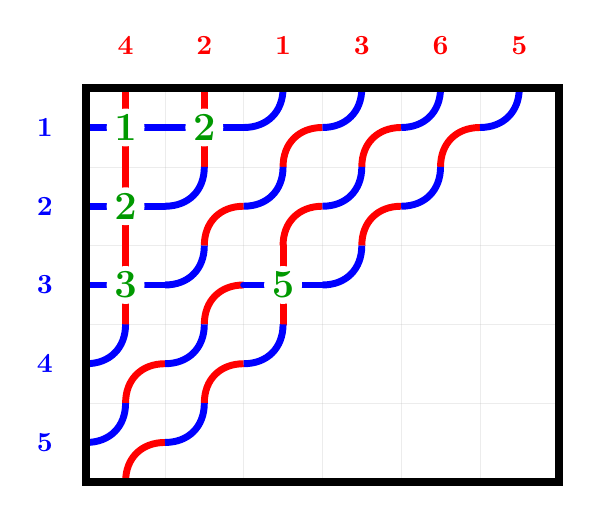
\begin{tikzpicture}[scale=1.0]
  \draw[lightgray, very thin, opacity=0.3] (0,1) -- (6,1);
  \draw[lightgray, very thin, opacity=0.3] (0,2) -- (6,2);
  \draw[lightgray, very thin, opacity=0.3] (0,3) -- (6,3);
  \draw[lightgray, very thin, opacity=0.3] (0,4) -- (6,4);
  \draw[lightgray, very thin, opacity=0.3] (0,5) -- (6,5);
  \draw[lightgray, very thin, opacity=0.3] (0,6) -- (6,6);
  \draw[lightgray, very thin, opacity=0.3] (0,1) -- (0,6);
  \draw[lightgray, very thin, opacity=0.3] (1,1) -- (1,6);
  \draw[lightgray, very thin, opacity=0.3] (2,1) -- (2,6);
  \draw[lightgray, very thin, opacity=0.3] (3,1) -- (3,6);
  \draw[lightgray, very thin, opacity=0.3] (4,1) -- (4,6);
  \draw[lightgray, very thin, opacity=0.3] (5,1) -- (5,6);
  \draw[lightgray, very thin, opacity=0.3] (6,1) -- (6,6);
  \draw[blue, line width=2.5pt, line cap=round] (0,5.5) -- (1,5.5);
  \draw[red, line width=2.5pt, line cap=round] (0.5,5) -- (0.5,6);
  \draw[blue, line width=2.5pt, line cap=round] (1,5.5) -- (2,5.5);
  \draw[red, line width=2.5pt, line cap=round] (1.5,5) -- (1.5,6);
  \draw[blue, line width=2.5pt] (2,5.5) .. controls (2.3,5.5) and (2.5,5.7) .. (2.5,6);
  \draw[red, line width=2.5pt] (2.5,5) .. controls (2.5,5.3) and (2.7,5.5) .. (3,5.5);
  \draw[blue, line width=2.5pt] (3,5.5) .. controls (3.3,5.5) and (3.5,5.7) .. (3.5,6);
  \draw[red, line width=2.5pt] (3.5,5) .. controls (3.5,5.3) and (3.7,5.5) .. (4,5.5);
  \draw[blue, line width=2.5pt] (4,5.5) .. controls (4.3,5.5) and (4.5,5.7) .. (4.5,6);
  \draw[red, line width=2.5pt] (4.5,5) .. controls (4.5,5.3) and (4.7,5.5) .. (5,5.5);
  \draw[blue, line width=2.5pt] (5,5.5) .. controls (5.3,5.5) and (5.5,5.7) .. (5.5,6);
  \draw[blue, line width=2.5pt, line cap=round] (0,4.5) -- (1,4.5);
  \draw[red, line width=2.5pt, line cap=round] (0.5,4) -- (0.5,5);
  \draw[blue, line width=2.5pt] (1,4.5) .. controls (1.3,4.5) and (1.5,4.7) .. (1.5,5);
  \draw[red, line width=2.5pt] (1.5,4) .. controls (1.5,4.3) and (1.7,4.5) .. (2,4.5);
  \draw[blue, line width=2.5pt] (2,4.5) .. controls (2.3,4.5) and (2.5,4.7) .. (2.5,5);
  \draw[red, line width=2.5pt] (2.5,4) .. controls (2.5,4.3) and (2.7,4.5) .. (3,4.5);
  \draw[blue, line width=2.5pt] (3,4.5) .. controls (3.3,4.5) and (3.5,4.7) .. (3.5,5);
  \draw[red, line width=2.5pt] (3.5,4) .. controls (3.5,4.3) and (3.7,4.5) .. (4,4.5);
  \draw[blue, line width=2.5pt] (4,4.5) .. controls (4.3,4.5) and (4.5,4.7) .. (4.5,5);
  \draw[blue, line width=2.5pt, line cap=round] (0,3.5) -- (1,3.5);
  \draw[red, line width=2.5pt, line cap=round] (0.5,3) -- (0.5,4);
  \draw[blue, line width=2.5pt] (1,3.5) .. controls (1.3,3.5) and (1.5,3.7) .. (1.5,4);
  \draw[red, line width=2.5pt] (1.5,3) .. controls (1.5,3.3) and (1.7,3.5) .. (2,3.5);
  \draw[blue, line width=2.5pt, line cap=round] (2,3.5) -- (3,3.5);
  \draw[red, line width=2.5pt, line cap=round] (2.5,3) -- (2.5,4);
  \draw[blue, line width=2.5pt] (3,3.5) .. controls (3.3,3.5) and (3.5,3.7) .. (3.5,4);
  \draw[blue, line width=2.5pt] (0,2.5) .. controls (0.3,2.5) and (0.5,2.7) .. (0.5,3);
  \draw[red, line width=2.5pt] (0.5,2) .. controls (0.5,2.3) and (0.7,2.5) .. (1,2.5);
  \draw[blue, line width=2.5pt] (1,2.5) .. controls (1.3,2.5) and (1.5,2.7) .. (1.5,3);
  \draw[red, line width=2.5pt] (1.5,2) .. controls (1.5,2.3) and (1.7,2.5) .. (2,2.5);
  \draw[blue, line width=2.5pt] (2,2.5) .. controls (2.3,2.5) and (2.5,2.7) .. (2.5,3);
  \draw[blue, line width=2.5pt] (0,1.5) .. controls (0.3,1.5) and (0.5,1.7) .. (0.5,2);
  \draw[red, line width=2.5pt] (0.5,1) .. controls (0.5,1.3) and (0.7,1.5) .. (1,1.5);
  \draw[blue, line width=2.5pt] (1,1.5) .. controls (1.3,1.5) and (1.5,1.7) .. (1.5,2);
  \node[font=\Large\bfseries, text=green!60!black, fill=white, inner sep=0.5pt, circle, transform shape] at (1.5,5.5) {2};
  \node[font=\Large\bfseries, text=green!60!black, fill=white, inner sep=0.5pt, circle, transform shape] at (0.5,4.5) {2};
  \node[font=\Large\bfseries, text=green!60!black, fill=white, inner sep=0.5pt, circle, transform shape] at (0.5,3.5) {3};
  \node[font=\Large\bfseries, text=green!60!black, fill=white, inner sep=0.5pt, circle, transform shape] at (0.5,5.5) {1};
  \node[font=\Large\bfseries, text=green!60!black, fill=white, inner sep=0.5pt, circle, transform shape] at (2.5,3.5) {5};
  \node[font=\bfseries, text=red, anchor=south] at (0.5,6.3) {4};
  \node[font=\bfseries, text=red, anchor=south] at (1.5,6.3) {2};
  \node[font=\bfseries, text=red, anchor=south] at (2.5,6.3) {1};
  \node[font=\bfseries, text=red, anchor=south] at (3.5,6.3) {3};
  \node[font=\bfseries, text=red, anchor=south] at (4.5,6.3) {6};
  \node[font=\bfseries, text=red, anchor=south] at (5.5,6.3) {5};
  \node[font=\bfseries, text=blue, anchor=east] at (-0.3,5.5) {1};
  \node[font=\bfseries, text=blue, anchor=east] at (-0.3,4.5) {2};
  \node[font=\bfseries, text=blue, anchor=east] at (-0.3,3.5) {3};
  \node[font=\bfseries, text=blue, anchor=east] at (-0.3,2.5) {4};
  \node[font=\bfseries, text=blue, anchor=east] at (-0.3,1.5) {5};
  \draw[black, line width=3.0pt] (0,1) rectangle (6,6);
\end{tikzpicture}
\end{figure}


The main benefit of this is that visualizing $\rtt_R(i,j)$ is easy. The pipes that pass through position $(i,j)$ are labeled $s$ and $q$ for some $s,q>0$. For a positive root in an unoccupied square, we will have the following labeling, where $q<s$:

\begin{center}
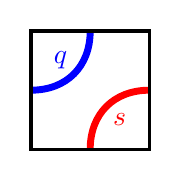
\begin{tikzpicture}[scale=1.5]
  % Draw the grid for a single square
  \draw[lightgray, very thin, opacity=0.3] (0,0) -- (1,0);
  \draw[lightgray, very thin, opacity=0.3] (0,1) -- (1,1);
  \draw[lightgray, very thin, opacity=0.3] (0,0) -- (0,1);
  \draw[lightgray, very thin, opacity=0.3] (1,0) -- (1,1);
  
  % Draw the elbow with two arcs
  % Blue arc (from left to top)
  \draw[blue, line width=2.5pt] (0,0.5) .. controls (0.3,0.5) and (0.5,0.7) .. (0.5,1);
  
  % Red arc (from bottom to right)
  \draw[red, line width=2.5pt] (0.5,0) .. controls (0.5,0.3) and (0.7,0.5) .. (1,0.5);
  
  % Labels
  \node[font=\bfseries, text=blue] at (0.25,0.75) {$q$};
  \node[font=\bfseries, text=red] at (0.75,0.25) {$s$};
  
  % Box around the grid
  \draw[black, line width=1.2pt] (0,0) rectangle (1,1);
\end{tikzpicture}
\end{center}

We observe that in the above RC graph, the position $(1,5)$ does not have this configuration. Placing a crossing there would create a negative root, and the pipes would cross twice. \emph{Note that this results in a collection of ordered pairs that is not an RC graph, if such a crossing exists.} For a valid RC graphs, only positive roots occur as crossings, and this happens if and only if pipes cross at most once.

\begin{figure}[h]
\centering
\caption{An invalid set of crossings causing pipes to cross more than once, caused by inserting a crossing at a negative root}
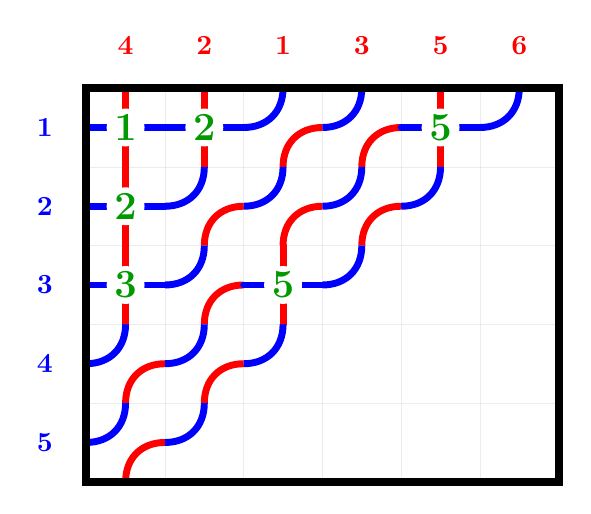
\begin{tikzpicture}[scale=1.0]
  \draw[lightgray, very thin, opacity=0.3] (0,1) -- (6,1);
  \draw[lightgray, very thin, opacity=0.3] (0,2) -- (6,2);
  \draw[lightgray, very thin, opacity=0.3] (0,3) -- (6,3);
  \draw[lightgray, very thin, opacity=0.3] (0,4) -- (6,4);
  \draw[lightgray, very thin, opacity=0.3] (0,5) -- (6,5);
  \draw[lightgray, very thin, opacity=0.3] (0,6) -- (6,6);
  \draw[lightgray, very thin, opacity=0.3] (0,1) -- (0,6);
  \draw[lightgray, very thin, opacity=0.3] (1,1) -- (1,6);
  \draw[lightgray, very thin, opacity=0.3] (2,1) -- (2,6);
  \draw[lightgray, very thin, opacity=0.3] (3,1) -- (3,6);
  \draw[lightgray, very thin, opacity=0.3] (4,1) -- (4,6);
  \draw[lightgray, very thin, opacity=0.3] (5,1) -- (5,6);
  \draw[lightgray, very thin, opacity=0.3] (6,1) -- (6,6);
  \draw[blue, line width=2.5pt, line cap=round] (0,5.5) -- (1,5.5);
  \draw[red, line width=2.5pt, line cap=round] (0.5,5) -- (0.5,6);
  \draw[blue, line width=2.5pt, line cap=round] (1,5.5) -- (2,5.5);
  \draw[red, line width=2.5pt, line cap=round] (1.5,5) -- (1.5,6);
  \draw[blue, line width=2.5pt] (2,5.5) .. controls (2.3,5.5) and (2.5,5.7) .. (2.5,6);
  \draw[red, line width=2.5pt] (2.5,5) .. controls (2.5,5.3) and (2.7,5.5) .. (3,5.5);
  \draw[blue, line width=2.5pt] (3,5.5) .. controls (3.3,5.5) and (3.5,5.7) .. (3.5,6);
  \draw[red, line width=2.5pt] (3.5,5) .. controls (3.5,5.3) and (3.7,5.5) .. (4,5.5);
  \draw[blue, line width=2.5pt, line cap=round] (4,5.5) -- (5,5.5);
  \draw[red, line width=2.5pt, line cap=round] (4.5,5) -- (4.5,6);
  \draw[blue, line width=2.5pt] (5,5.5) .. controls (5.3,5.5) and (5.5,5.7) .. (5.5,6);
  \draw[blue, line width=2.5pt, line cap=round] (0,4.5) -- (1,4.5);
  \draw[red, line width=2.5pt, line cap=round] (0.5,4) -- (0.5,5);
  \draw[blue, line width=2.5pt] (1,4.5) .. controls (1.3,4.5) and (1.5,4.7) .. (1.5,5);
  \draw[red, line width=2.5pt] (1.5,4) .. controls (1.5,4.3) and (1.7,4.5) .. (2,4.5);
  \draw[blue, line width=2.5pt] (2,4.5) .. controls (2.3,4.5) and (2.5,4.7) .. (2.5,5);
  \draw[red, line width=2.5pt] (2.5,4) .. controls (2.5,4.3) and (2.7,4.5) .. (3,4.5);
  \draw[blue, line width=2.5pt] (3,4.5) .. controls (3.3,4.5) and (3.5,4.7) .. (3.5,5);
  \draw[red, line width=2.5pt] (3.5,4) .. controls (3.5,4.3) and (3.7,4.5) .. (4,4.5);
  \draw[blue, line width=2.5pt] (4,4.5) .. controls (4.3,4.5) and (4.5,4.7) .. (4.5,5);
  \draw[blue, line width=2.5pt, line cap=round] (0,3.5) -- (1,3.5);
  \draw[red, line width=2.5pt, line cap=round] (0.5,3) -- (0.5,4);
  \draw[blue, line width=2.5pt] (1,3.5) .. controls (1.3,3.5) and (1.5,3.7) .. (1.5,4);
  \draw[red, line width=2.5pt] (1.5,3) .. controls (1.5,3.3) and (1.7,3.5) .. (2,3.5);
  \draw[blue, line width=2.5pt, line cap=round] (2,3.5) -- (3,3.5);
  \draw[red, line width=2.5pt, line cap=round] (2.5,3) -- (2.5,4);
  \draw[blue, line width=2.5pt] (3,3.5) .. controls (3.3,3.5) and (3.5,3.7) .. (3.5,4);
  \draw[blue, line width=2.5pt] (0,2.5) .. controls (0.3,2.5) and (0.5,2.7) .. (0.5,3);
  \draw[red, line width=2.5pt] (0.5,2) .. controls (0.5,2.3) and (0.7,2.5) .. (1,2.5);
  \draw[blue, line width=2.5pt] (1,2.5) .. controls (1.3,2.5) and (1.5,2.7) .. (1.5,3);
  \draw[red, line width=2.5pt] (1.5,2) .. controls (1.5,2.3) and (1.7,2.5) .. (2,2.5);
  \draw[blue, line width=2.5pt] (2,2.5) .. controls (2.3,2.5) and (2.5,2.7) .. (2.5,3);
  \draw[blue, line width=2.5pt] (0,1.5) .. controls (0.3,1.5) and (0.5,1.7) .. (0.5,2);
  \draw[red, line width=2.5pt] (0.5,1) .. controls (0.5,1.3) and (0.7,1.5) .. (1,1.5);
  \draw[blue, line width=2.5pt] (1,1.5) .. controls (1.3,1.5) and (1.5,1.7) .. (1.5,2);
  \node[font=\Large\bfseries, text=green!60!black, fill=white, inner sep=0.5pt, circle, transform shape] at (1.5,5.5) {2};
  \node[font=\Large\bfseries, text=green!60!black, fill=white, inner sep=0.5pt, circle, transform shape] at (0.5,4.5) {2};
  \node[font=\Large\bfseries, text=green!60!black, fill=white, inner sep=0.5pt, circle, transform shape] at (4.5,5.5) {5};
  \node[font=\Large\bfseries, text=green!60!black, fill=white, inner sep=0.5pt, circle, transform shape] at (0.5,3.5) {3};
  \node[font=\Large\bfseries, text=green!60!black, fill=white, inner sep=0.5pt, circle, transform shape] at (0.5,5.5) {1};
  \node[font=\Large\bfseries, text=green!60!black, fill=white, inner sep=0.5pt, circle, transform shape] at (2.5,3.5) {5};
  \node[font=\bfseries, text=red, anchor=south] at (0.5,6.3) {4};
  \node[font=\bfseries, text=red, anchor=south] at (1.5,6.3) {2};
  \node[font=\bfseries, text=red, anchor=south] at (2.5,6.3) {1};
  \node[font=\bfseries, text=red, anchor=south] at (3.5,6.3) {3};
  \node[font=\bfseries, text=red, anchor=south] at (4.5,6.3) {5};
  \node[font=\bfseries, text=red, anchor=south] at (5.5,6.3) {6};
  \node[font=\bfseries, text=blue, anchor=east] at (-0.3,5.5) {1};
  \node[font=\bfseries, text=blue, anchor=east] at (-0.3,4.5) {2};
  \node[font=\bfseries, text=blue, anchor=east] at (-0.3,3.5) {3};
  \node[font=\bfseries, text=blue, anchor=east] at (-0.3,2.5) {4};
  \node[font=\bfseries, text=blue, anchor=east] at (-0.3,1.5) {5};
  \draw[black, line width=3.0pt] (0,1) rectangle (6,6);
\end{tikzpicture}
\end{figure}

\subsection{Bijection with inversion tableaux}


\cite{axelrodfreed2025inversionstableaux}

\begin{definition}
An \emph{inversion tableau} is a function $T:(\mathbb{Z}_{> 0}\times \mathbb{Z}_{> 0})^+\to \mathbb{Z}_{>0}\cup\{-\infty\}$ such that only finitely many values are nonzero. Note $-\infty < a$ for all $a$, including $a=-\infty$.  In addition, we have the following requirements:
\begin{enumerate}
\item For each $i<j<k$ we have either
$$T(i,j)\leq T(i,k)< T(j,k)$$
or
$$T(j,k)< T(i,k)\leq T(i,j)$$
\item For each $i\geq 1$ we have
$$T(i, i+1)\leq i$$
\end{enumerate}
If $R$ is an RC graph, we define an associated inversions tableau $T_R$ as in the proof of \cite[Theorem~3.13]{axelrodfreed2025inversionstableaux} by
$$T_R(a,b) = \begin{cases}
 i& \text{if } (i,j) \in R\mbox{ and }(a,b)=\rtt_R^{-1}(i,j)\\
 -\infty& \text{otherwise}
 \end{cases}$$
\end{definition}

\begin{lemma} \label{lemma:rowcol}
We have the following for an RC graph $R$:
\begin{enumerate}
	\item Suppose $(i, j), (i, j+1)\in R$. Then $\rtt_R(i, j) = (a, c)$ and $\rtt_R(i, j+1) = (a, b)$ for some $a < b < c$.
	\item Suppose $(i, j), (i+1, j)\in R$. Then $\rtt_R(i, j) = (a, c)$ and $\rtt_R(i+1, j) = (b, c)$ for some $a < b < c$.
\end{enumerate}

\end{lemma}

\subsection{Zeroing out the last row}

We proceed now to define a product on $\BRC$ turning it into a ring. To do this, we need to be able to define a function $Z:\BRC\to\BRC$ trimming empty rows from the bottom instead of from the top. This is far more complicated.


%\begin{algorithm} 
%Given an RC graph $R$, a positive integer $k$, and a sequence of positive integers $k\geq i_1\geq \cdots \geq i_m$, we define an insertion algorithm similar to that in \cite{kogan2002proof} but in a sense ``backwards'' that will be more suitable to our purposes. The result is an RC graph $R'$ with additional elements $(i_1,j_1),\ldots,(i_m,j_m)$ such that $w(R)$ is related to $w(R')$ by the complete symmetric polynomial $k$-Pieri relation.
%
%We maintain a list $(a_1,b_1),\ldots,(a_p,b_p)$ such that $a_1\leq\cdots \leq a_p\leq k$ and $b_1,\ldots,b_p>k$ are all distinct. As in Kogan and Kumar's algorithm, the list is initially empty.
%
%Starting in row $i_1$, find the leftmost position $(i_1, j)$ such that $(i_1,j)\notin R$ and either $\rtt_R(i_1, j)=t_s - t_q$, where $s\leq k<q$ and $q\neq b_j$ for any $j$, or $\rtt_R(i_1, j) = \pm t_q \mp t_{b_i}$, where $q>k$ and $q\neq b_j$ for any $j$. Add $(i_1,j)$ to $R$ to obtain an interim set $R'$, and to the sequence we either add $(s,q)$ in the first case or $(a_i, q)$ just before $(a_i,b_i)$ in the second case.
%
%In Kogan and Kumar's algorithm, we would proceed further in the same row before rectifying. However, in our algorithm we must rectify immediately if $R'$ is not an RC graph. This will happen if there is some $(i',j')\in R'$, necessarily before $(i_1, j)$ in the grid ordering, such that $\rtt_{R'}(i',j')$ is a negative root. This negative root is either $t_{b_i}-t_{a_i}$ for some $i$ or $\pm t_{b_i} \mp t_{b_q}$ for some $i,q$ such that $a_i=a_q$. Delete this bad element from $R'$ and insert via the procedure above to replace it. Apply this recursively until the result is an RC graph.  
%
%After the rectification, proceed with insertion as in the beginning until the list of $i_1,\ldots,i_m$ is exhausted.
%\end{algorithm}

% Define the main algorithm
\begin{algorithm} 
	\caption{RC insertion algorithm}
	\label{algorithm:insertion}
	\begin{algorithmic}[1]
		\State \textbf{Input:} An RC graph $R$, parameter $k$, and sequence $k\geq i_1 \geq i_2 \geq \cdots \geq i_m \geq 1$.
		\State \textbf{Output:} A modified RC graph $R'$.
		\State \textbf{Initialize:} Let $L \gets [\,]$ (empty list of pairs $(a, b)$ where $a \leq k < b$), and $r\gets [\,]$ (empty list).
		\For{each $i \in (i_1, \ldots, i_m)$}
		\State Find leftmost position $(i, j) \notin R$ in row $i$ satisfying $j>j'$ for all $(i,j')\in r$ such that either:
		\State \quad a) $\rtt_R(i, j) = (s, q)$ where $s \leq k < q$ and $q \notin \{b \mid (a, b) \in L\}$.
		\State \quad b) $\rtt_R(i, j) = (b_r, q)$ where $q > k$, $b_r<q$, and $q \notin \{b \mid (a, b) \in L\}$.
		\State $R \gets R \cup \{(i, j)\}$ and $r\gets r\cup \{(i, j)\}$
		\State Update $L$ by adding $(s, q)$ or replacing $(a_r, b_r)$ with $(a_r, q)$ and $(a_r, b_r)$.
		\State $(R, L) \gets \textproc{Rectify}(R, L, i - 1)$ (Algorithm \ref{algorithm:rectify})
		\EndFor
		\State \Return $R$
	\end{algorithmic}
\end{algorithm}

% Define the Subroutine
\begin{algorithm}
	\caption{Subroutine: Rectify}
	\label{algorithm:rectify}
	\begin{algorithmic}[1]
		\Procedure{Rectify}{$R, L, i$}
		\If{$R$ is an RC graph or $i = 0$} 
		\State \Return $(R, L)$
		\EndIf
		\For{minimal $j$ such that $(i,j) \in R$ and $\rtt_R(i, j) \in \Phi^-$}
		\State $R \gets R \setminus \{(i, j)\}$
		\State Let $\rtt_R(i, j) = (q, s)$
		\If{$(s, q) \in L$}
		\State Remove $(s, q)$ from $L$
		\Else
		\State Remove $(a_r, q)$ from $L$, where $(a_r, q),(a_r,s)\in L$
		\EndIf
		\State Perform new insertion step at row $i$ using criteria from Algorithm \ref{algorithm:insertion} Step 5.
		\EndFor
		\State \Return \Call{Rectify}{$R, L, i - 1$}
		\EndProcedure
	\end{algorithmic}
\end{algorithm}


\begin{algorithm}[H]
	\caption{Map $Z(R, n)$ zeroing out row $n$}
	\label{algorithm:zero}
	\begin{algorithmic}[1]
		\State \textbf{Input:} A bounded RC graph $(R, n)$ with row $n$ empty.
		\State \textbf{Output:} A bounded RC graph $(R', n-1)$ such that $|R'|=|R|$ and $\wof{R}\downvar{n} \wof{R'}$.
		
		\If{$(R, n-1)$ is a valid bounded RC graph}
		\State \Return $(R, n-1)$
		\Else
		\State Let $R_0 \gets R$.
		\State Find the maximal $p$ and sequence $\{(i_m, j_m)\}_{m=1}^p$ such that:
		\State \quad $\rtt_{R_{m-1}}(i_m, j_m) = (n+m-1,n+m)$ for each $m$, where $R_m = R_{m-1}\setminus\{(i_m, j_m)\}$ for each $m\geq 1$.
		\State $R^- \gets R \setminus \{(i_1, j_1), \ldots, (i_p, j_p)\}$.
		\State Let $I \gets (i_1, i_2, \ldots, i_p)$.
		\State $D \gets R^- \cup \{(n, 1), (n, 2), \ldots, (n, p)\}$.
		\State $D' \gets \textproc{Insert}(D, n-1, I)$ \Comment{Using Algorithm \ref{algorithm:insertion}}
		\State $R' \gets \{(i, j) \in D' \mid i < n\}$.
		\State \Return $(R', n-1)$.
		\EndIf
	\end{algorithmic}
\end{algorithm}

See Figure \ref{fig:zeroing} for an example of the zeroing operation (Algorithm \ref{algorithm:zero}).

\begin{figure}[htbp]
\centering

% First diagram
\begin{minipage}{0.45\textwidth}
\centering
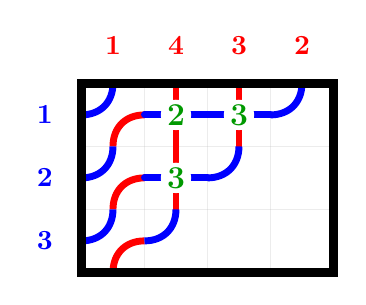
\begin{tikzpicture}[scale=0.8]
  \draw[lightgray, very thin, opacity=0.3] (0,1) -- (4,1);
  \draw[lightgray, very thin, opacity=0.3] (0,2) -- (4,2);
  \draw[lightgray, very thin, opacity=0.3] (0,3) -- (4,3);
  \draw[lightgray, very thin, opacity=0.3] (0,4) -- (4,4);
  \draw[lightgray, very thin, opacity=0.3] (0,1) -- (0,4);
  \draw[lightgray, very thin, opacity=0.3] (1,1) -- (1,4);
  \draw[lightgray, very thin, opacity=0.3] (2,1) -- (2,4);
  \draw[lightgray, very thin, opacity=0.3] (3,1) -- (3,4);
  \draw[lightgray, very thin, opacity=0.3] (4,1) -- (4,4);
  \draw[blue, line width=2.5pt] (0,3.5) .. controls (0.3,3.5) and (0.5,3.7) .. (0.5,4);
  \draw[red, line width=2.5pt] (0.5,3) .. controls (0.5,3.3) and (0.7,3.5) .. (1,3.5);
  \draw[blue, line width=2.5pt, line cap=round] (1,3.5) -- (2,3.5);
  \draw[red, line width=2.5pt, line cap=round] (1.5,3) -- (1.5,4);
  \draw[blue, line width=2.5pt, line cap=round] (2,3.5) -- (3,3.5);
  \draw[red, line width=2.5pt, line cap=round] (2.5,3) -- (2.5,4);
  \draw[blue, line width=2.5pt] (3,3.5) .. controls (3.3,3.5) and (3.5,3.7) .. (3.5,4);
  \draw[blue, line width=2.5pt] (0,2.5) .. controls (0.3,2.5) and (0.5,2.7) .. (0.5,3);
  \draw[red, line width=2.5pt] (0.5,2) .. controls (0.5,2.3) and (0.7,2.5) .. (1,2.5);
  \draw[blue, line width=2.5pt, line cap=round] (1,2.5) -- (2,2.5);
  \draw[red, line width=2.5pt, line cap=round] (1.5,2) -- (1.5,3);
  \draw[blue, line width=2.5pt] (2,2.5) .. controls (2.3,2.5) and (2.5,2.7) .. (2.5,3);
  \draw[blue, line width=2.5pt] (0,1.5) .. controls (0.3,1.5) and (0.5,1.7) .. (0.5,2);
  \draw[red, line width=2.5pt] (0.5,1) .. controls (0.5,1.3) and (0.7,1.5) .. (1,1.5);
  \draw[blue, line width=2.5pt] (1,1.5) .. controls (1.3,1.5) and (1.5,1.7) .. (1.5,2);
  \node[font=\Large\bfseries, text=green!60!black, fill=white, inner sep=0.5pt, circle, transform shape] at (1.5,3.5) {2};
  \node[font=\Large\bfseries, text=green!60!black, fill=white, inner sep=0.5pt, circle, transform shape] at (2.5,3.5) {3};
  \node[font=\Large\bfseries, text=green!60!black, fill=white, inner sep=0.5pt, circle, transform shape] at (1.5,2.5) {3};
  \node[font=\bfseries, text=red, anchor=south] at (0.5,4.3) {1};
  \node[font=\bfseries, text=red, anchor=south] at (1.5,4.3) {4};
  \node[font=\bfseries, text=red, anchor=south] at (2.5,4.3) {3};
  \node[font=\bfseries, text=red, anchor=south] at (3.5,4.3) {2};
  \node[font=\bfseries, text=blue, anchor=east] at (-0.3,3.5) {1};
  \node[font=\bfseries, text=blue, anchor=east] at (-0.3,2.5) {2};
  \node[font=\bfseries, text=blue, anchor=east] at (-0.3,1.5) {3};
  \draw[black, line width=3.0pt] (0,1) rectangle (4,4);
\end{tikzpicture}
\caption*{(a) Initial RC graph $R$}
\end{minipage}
\hfill
% Second diagram
\begin{minipage}{0.45\textwidth}
\centering
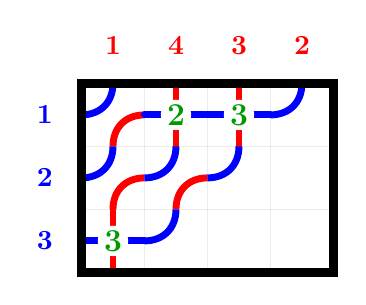
\begin{tikzpicture}[scale=0.8]
  \draw[lightgray, very thin, opacity=0.3] (0,1) -- (4,1);
  \draw[lightgray, very thin, opacity=0.3] (0,2) -- (4,2);
  \draw[lightgray, very thin, opacity=0.3] (0,3) -- (4,3);
  \draw[lightgray, very thin, opacity=0.3] (0,4) -- (4,4);
  \draw[lightgray, very thin, opacity=0.3] (0,1) -- (0,4);
  \draw[lightgray, very thin, opacity=0.3] (1,1) -- (1,4);
  \draw[lightgray, very thin, opacity=0.3] (2,1) -- (2,4);
  \draw[lightgray, very thin, opacity=0.3] (3,1) -- (3,4);
  \draw[lightgray, very thin, opacity=0.3] (4,1) -- (4,4);
  \draw[blue, line width=2.5pt] (0,3.5) .. controls (0.3,3.5) and (0.5,3.7) .. (0.5,4);
  \draw[red, line width=2.5pt] (0.5,3) .. controls (0.5,3.3) and (0.7,3.5) .. (1,3.5);
  \draw[blue, line width=2.5pt, line cap=round] (1,3.5) -- (2,3.5);
  \draw[red, line width=2.5pt, line cap=round] (1.5,3) -- (1.5,4);
  \draw[blue, line width=2.5pt, line cap=round] (2,3.5) -- (3,3.5);
  \draw[red, line width=2.5pt, line cap=round] (2.5,3) -- (2.5,4);
  \draw[blue, line width=2.5pt] (3,3.5) .. controls (3.3,3.5) and (3.5,3.7) .. (3.5,4);
  \draw[blue, line width=2.5pt] (0,2.5) .. controls (0.3,2.5) and (0.5,2.7) .. (0.5,3);
  \draw[red, line width=2.5pt] (0.5,2) .. controls (0.5,2.3) and (0.7,2.5) .. (1,2.5);
  \draw[blue, line width=2.5pt] (1,2.5) .. controls (1.3,2.5) and (1.5,2.7) .. (1.5,3);
  \draw[red, line width=2.5pt] (1.5,2) .. controls (1.5,2.3) and (1.7,2.5) .. (2,2.5);
  \draw[blue, line width=2.5pt] (2,2.5) .. controls (2.3,2.5) and (2.5,2.7) .. (2.5,3);
  \draw[blue, line width=2.5pt, line cap=round] (0,1.5) -- (1,1.5);
  \draw[red, line width=2.5pt, line cap=round] (0.5,1) -- (0.5,2);
  \draw[blue, line width=2.5pt] (1,1.5) .. controls (1.3,1.5) and (1.5,1.7) .. (1.5,2);
  \node[font=\Large\bfseries, text=green!60!black, fill=white, inner sep=0.5pt, circle, transform shape] at (0.5,1.5) {3};
  \node[font=\Large\bfseries, text=green!60!black, fill=white, inner sep=0.5pt, circle, transform shape] at (1.5,3.5) {2};
  \node[font=\Large\bfseries, text=green!60!black, fill=white, inner sep=0.5pt, circle, transform shape] at (2.5,3.5) {3};
  \node[font=\bfseries, text=red, anchor=south] at (0.5,4.3) {1};
  \node[font=\bfseries, text=red, anchor=south] at (1.5,4.3) {4};
  \node[font=\bfseries, text=red, anchor=south] at (2.5,4.3) {3};
  \node[font=\bfseries, text=red, anchor=south] at (3.5,4.3) {2};
  \node[font=\bfseries, text=blue, anchor=east] at (-0.3,3.5) {1};
  \node[font=\bfseries, text=blue, anchor=east] at (-0.3,2.5) {2};
  \node[font=\bfseries, text=blue, anchor=east] at (-0.3,1.5) {3};
  \draw[black, line width=3.0pt] (0,1) rectangle (4,4);
\end{tikzpicture}
\caption*{(b) After deleting $(2,2)$ with $\rtt_R(2,2)=\alpha_3$ and moving to row $3$}
\end{minipage}

\vspace{1em}

% Third diagram
\begin{minipage}{0.45\textwidth}
\centering
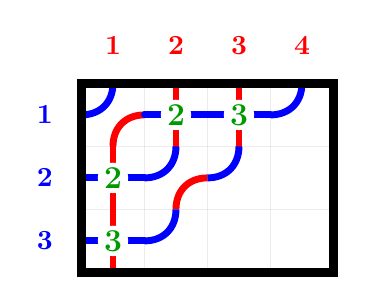
\begin{tikzpicture}[scale=0.8]
  \draw[lightgray, very thin, opacity=0.3] (0,1) -- (4,1);
  \draw[lightgray, very thin, opacity=0.3] (0,2) -- (4,2);
  \draw[lightgray, very thin, opacity=0.3] (0,3) -- (4,3);
  \draw[lightgray, very thin, opacity=0.3] (0,4) -- (4,4);
  \draw[lightgray, very thin, opacity=0.3] (0,1) -- (0,4);
  \draw[lightgray, very thin, opacity=0.3] (1,1) -- (1,4);
  \draw[lightgray, very thin, opacity=0.3] (2,1) -- (2,4);
  \draw[lightgray, very thin, opacity=0.3] (3,1) -- (3,4);
  \draw[lightgray, very thin, opacity=0.3] (4,1) -- (4,4);
  \draw[blue, line width=2.5pt] (0,3.5) .. controls (0.3,3.5) and (0.5,3.7) .. (0.5,4);
  \draw[red, line width=2.5pt] (0.5,3) .. controls (0.5,3.3) and (0.7,3.5) .. (1,3.5);
  \draw[blue, line width=2.5pt, line cap=round] (1,3.5) -- (2,3.5);
  \draw[red, line width=2.5pt, line cap=round] (1.5,3) -- (1.5,4);
  \draw[blue, line width=2.5pt, line cap=round] (2,3.5) -- (3,3.5);
  \draw[red, line width=2.5pt, line cap=round] (2.5,3) -- (2.5,4);
  \draw[blue, line width=2.5pt] (3,3.5) .. controls (3.3,3.5) and (3.5,3.7) .. (3.5,4);
  \draw[blue, line width=2.5pt, line cap=round] (0,2.5) -- (1,2.5);
  \draw[red, line width=2.5pt, line cap=round] (0.5,2) -- (0.5,3);
  \draw[blue, line width=2.5pt] (1,2.5) .. controls (1.3,2.5) and (1.5,2.7) .. (1.5,3);
  \draw[red, line width=2.5pt] (1.5,2) .. controls (1.5,2.3) and (1.7,2.5) .. (2,2.5);
  \draw[blue, line width=2.5pt] (2,2.5) .. controls (2.3,2.5) and (2.5,2.7) .. (2.5,3);
  \draw[blue, line width=2.5pt, line cap=round] (0,1.5) -- (1,1.5);
  \draw[red, line width=2.5pt, line cap=round] (0.5,1) -- (0.5,2);
  \draw[blue, line width=2.5pt] (1,1.5) .. controls (1.3,1.5) and (1.5,1.7) .. (1.5,2);
  \node[font=\Large\bfseries, text=green!60!black, fill=white, inner sep=0.5pt, circle, transform shape] at (0.5,1.5) {3};
  \node[font=\Large\bfseries, text=green!60!black, fill=white, inner sep=0.5pt, circle, transform shape] at (1.5,3.5) {2};
  \node[font=\Large\bfseries, text=green!60!black, fill=white, inner sep=0.5pt, circle, transform shape] at (2.5,3.5) {3};
  \node[font=\Large\bfseries, text=green!60!black, fill=white, inner sep=0.5pt, circle, transform shape] at (0.5,2.5) {2};
  \node[font=\bfseries, text=red, anchor=south] at (0.5,4.3) {1};
  \node[font=\bfseries, text=red, anchor=south] at (1.5,4.3) {2};
  \node[font=\bfseries, text=red, anchor=south] at (2.5,4.3) {3};
  \node[font=\bfseries, text=red, anchor=south] at (3.5,4.3) {4};
  \node[font=\bfseries, text=blue, anchor=east] at (-0.3,3.5) {1};
  \node[font=\bfseries, text=blue, anchor=east] at (-0.3,2.5) {2};
  \node[font=\bfseries, text=blue, anchor=east] at (-0.3,1.5) {3};
  \draw[black, line width=3.0pt] (0,1) rectangle (4,4);
\end{tikzpicture}
\caption*{(c) After insertion with $i_1=2$}
\end{minipage}
\hfill
% Fourth diagram
\begin{minipage}{0.45\textwidth}
\centering
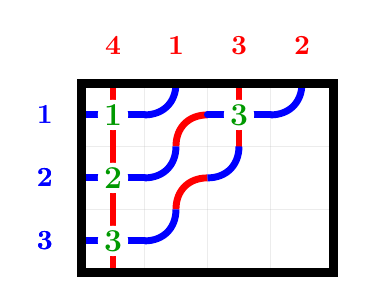
\begin{tikzpicture}[scale=0.8]
  \draw[lightgray, very thin, opacity=0.3] (0,1) -- (4,1);
  \draw[lightgray, very thin, opacity=0.3] (0,2) -- (4,2);
  \draw[lightgray, very thin, opacity=0.3] (0,3) -- (4,3);
  \draw[lightgray, very thin, opacity=0.3] (0,4) -- (4,4);
  \draw[lightgray, very thin, opacity=0.3] (0,1) -- (0,4);
  \draw[lightgray, very thin, opacity=0.3] (1,1) -- (1,4);
  \draw[lightgray, very thin, opacity=0.3] (2,1) -- (2,4);
  \draw[lightgray, very thin, opacity=0.3] (3,1) -- (3,4);
  \draw[lightgray, very thin, opacity=0.3] (4,1) -- (4,4);
  \draw[blue, line width=2.5pt, line cap=round] (0,3.5) -- (1,3.5);
  \draw[red, line width=2.5pt, line cap=round] (0.5,3) -- (0.5,4);
  \draw[blue, line width=2.5pt] (1,3.5) .. controls (1.3,3.5) and (1.5,3.7) .. (1.5,4);
  \draw[red, line width=2.5pt] (1.5,3) .. controls (1.5,3.3) and (1.7,3.5) .. (2,3.5);
  \draw[blue, line width=2.5pt, line cap=round] (2,3.5) -- (3,3.5);
  \draw[red, line width=2.5pt, line cap=round] (2.5,3) -- (2.5,4);
  \draw[blue, line width=2.5pt] (3,3.5) .. controls (3.3,3.5) and (3.5,3.7) .. (3.5,4);
  \draw[blue, line width=2.5pt, line cap=round] (0,2.5) -- (1,2.5);
  \draw[red, line width=2.5pt, line cap=round] (0.5,2) -- (0.5,3);
  \draw[blue, line width=2.5pt] (1,2.5) .. controls (1.3,2.5) and (1.5,2.7) .. (1.5,3);
  \draw[red, line width=2.5pt] (1.5,2) .. controls (1.5,2.3) and (1.7,2.5) .. (2,2.5);
  \draw[blue, line width=2.5pt] (2,2.5) .. controls (2.3,2.5) and (2.5,2.7) .. (2.5,3);
  \draw[blue, line width=2.5pt, line cap=round] (0,1.5) -- (1,1.5);
  \draw[red, line width=2.5pt, line cap=round] (0.5,1) -- (0.5,2);
  \draw[blue, line width=2.5pt] (1,1.5) .. controls (1.3,1.5) and (1.5,1.7) .. (1.5,2);
  \node[font=\Large\bfseries, text=green!60!black, fill=white, inner sep=0.5pt, circle, transform shape] at (0.5,1.5) {3};
  \node[font=\Large\bfseries, text=green!60!black, fill=white, inner sep=0.5pt, circle, transform shape] at (0.5,3.5) {1};
  \node[font=\Large\bfseries, text=green!60!black, fill=white, inner sep=0.5pt, circle, transform shape] at (2.5,3.5) {3};
  \node[font=\Large\bfseries, text=green!60!black, fill=white, inner sep=0.5pt, circle, transform shape] at (0.5,2.5) {2};
  \node[font=\bfseries, text=red, anchor=south] at (0.5,4.3) {4};
  \node[font=\bfseries, text=red, anchor=south] at (1.5,4.3) {1};
  \node[font=\bfseries, text=red, anchor=south] at (2.5,4.3) {3};
  \node[font=\bfseries, text=red, anchor=south] at (3.5,4.3) {2};
  \node[font=\bfseries, text=blue, anchor=east] at (-0.3,3.5) {1};
  \node[font=\bfseries, text=blue, anchor=east] at (-0.3,2.5) {2};
  \node[font=\bfseries, text=blue, anchor=east] at (-0.3,1.5) {3};
  \node[font=\bfseries, text=blue, anchor=east] at (-0.3,2.5) {2};
  \node[font=\bfseries, text=blue, anchor=east] at (-0.3,1.5) {3};
  \draw[black, line width=3.0pt] (0,1) rectangle (4,4);
\end{tikzpicture}
\caption*{(d) After rectification}
\end{minipage}

\vspace{1em}

% Fifth diagram
\begin{minipage}{0.45\textwidth}
\centering
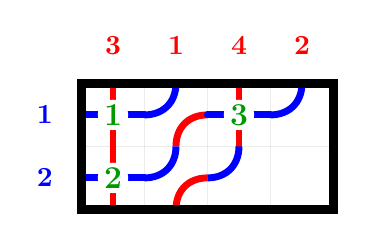
\begin{tikzpicture}[scale=0.8]
  \draw[lightgray, very thin, opacity=0.3] (0,2) -- (4,2);
  \draw[lightgray, very thin, opacity=0.3] (0,3) -- (4,3);
  \draw[lightgray, very thin, opacity=0.3] (0,4) -- (4,4);
  \draw[lightgray, very thin, opacity=0.3] (0,2) -- (0,4);
  \draw[lightgray, very thin, opacity=0.3] (1,2) -- (1,4);
  \draw[lightgray, very thin, opacity=0.3] (2,2) -- (2,4);
  \draw[lightgray, very thin, opacity=0.3] (3,2) -- (3,4);
  \draw[lightgray, very thin, opacity=0.3] (4,2) -- (4,4);
  \draw[blue, line width=2.5pt, line cap=round] (0,3.5) -- (1,3.5);
  \draw[red, line width=2.5pt, line cap=round] (0.5,3) -- (0.5,4);
  \draw[blue, line width=2.5pt] (1,3.5) .. controls (1.3,3.5) and (1.5,3.7) .. (1.5,4);
  \draw[red, line width=2.5pt] (1.5,3) .. controls (1.5,3.3) and (1.7,3.5) .. (2,3.5);
  \draw[blue, line width=2.5pt, line cap=round] (2,3.5) -- (3,3.5);
  \draw[red, line width=2.5pt, line cap=round] (2.5,3) -- (2.5,4);
  \draw[blue, line width=2.5pt] (3,3.5) .. controls (3.3,3.5) and (3.5,3.7) .. (3.5,4);
  \draw[blue, line width=2.5pt, line cap=round] (0,2.5) -- (1,2.5);
  \draw[red, line width=2.5pt, line cap=round] (0.5,2) -- (0.5,3);
  \draw[blue, line width=2.5pt] (1,2.5) .. controls (1.3,2.5) and (1.5,2.7) .. (1.5,3);
  \draw[red, line width=2.5pt] (1.5,2) .. controls (1.5,2.3) and (1.7,2.5) .. (2,2.5);
  \draw[blue, line width=2.5pt] (2,2.5) .. controls (2.3,2.5) and (2.5,2.7) .. (2.5,3);
  \node[font=\Large\bfseries, text=green!60!black, fill=white, inner sep=0.5pt, circle, transform shape] at (0.5,3.5) {1};
  \node[font=\Large\bfseries, text=green!60!black, fill=white, inner sep=0.5pt, circle, transform shape] at (2.5,3.5) {3};
  \node[font=\Large\bfseries, text=green!60!black, fill=white, inner sep=0.5pt, circle, transform shape] at (0.5,2.5) {2};
  \node[font=\bfseries, text=red, anchor=south] at (0.5,4.3) {3};
  \node[font=\bfseries, text=red, anchor=south] at (1.5,4.3) {1};
  \node[font=\bfseries, text=red, anchor=south] at (2.5,4.3) {4};
  \node[font=\bfseries, text=red, anchor=south] at (3.5,4.3) {2};
  \node[font=\bfseries, text=blue, anchor=east] at (-0.3,3.5) {1};
  \node[font=\bfseries, text=blue, anchor=east] at (-0.3,2.5) {2};
  \draw[black, line width=3.0pt] (0,2) rectangle (4,4);
\end{tikzpicture}
\caption*{(e) Final result $\zeromap(R,3)=(R',2)$ after removing row 3}
\end{minipage}

\caption{Step-by-step computation of $\zeromap(R, 3)$ for $R=\{(1,2),(1,3),(2,2)\}$.}
\label{fig:zeroing}
\end{figure}


\begin{lemma} \label{lemma:insertworks}
Given an RC graph $R$, an integer $k$, and $k\geq i_1\geq\cdots\geq i_m\geq 1$, Algorithm \ref{algorithm:insertion} produces a valid RC graph $R'$ satisfying
$$\wtt_i(R') = \wtt_i(R) + \#\{j \mid i_j = i\}$$
and
$$\wof{R}\Tom{k} \wof{R'}$$
\end{lemma}
\begin{proof}
Set $R_0=R$ to be the initial RC graph. We claim that given $R$ and $L$ at the start of iteration $p$ of the main loop, we have that $R$ is a valid RC graph satisfying
$$\wtt_i(R) = \wtt_i(R_0) + \#\{j \leq p-1 \mid i_j = i\}$$
and
$$\wof{R} = \wof{R_0}t_{a_1b_1}\cdots t_{a_{p-1}b_{p-1}}$$
where $L=[(a_1,b_1),\ldots,(a_p,b_p)]$. This is clear for $p=1$. For larger $p$, suppose we are inserting at row $i_p$. If we are in case (a) of Step 5, then adding $(i_p,j)$ to $R$ adds the root $t_s - t_q$ to the inversion set of $\wof{R}$, and multiplying by $t_{sq}$ gives the desired result. If we are in case (b) of Step 5, then adding $(i_p,j)$ to $R$ results in multiplication by $t_{b_rq}$. This commutes past the other reflections to meet $t_{a_rb_r}$. We thus have the situation
$$t_{a_rb_r}t_{b_rq} = t_{a_rq}t_{a_rb_r}$$
This ensures that the product remains as desired if the RC graph is valid. However, the condition that the RC graph $R$ be valid is not guaranteed after this step, so we must rectify. Suppose we must rectify at row $i - 1$. We find a negative root $(i-1, j')$ which must have been created by the insertion, and hence by the strong exchange property equal to $\rtt_R(i, j)$ that was inserted. Removing this root (from both the graph and from $L$) returns us to the original permutation at the beginning of the iteration, and performing the insert at row $i-1$ adds a new positive root, giving the desired result on the permutation. The weight is unchanged since we removed and added one crossing in row $i-1$. If the algorithm ends here, we have instead multiplied by the new reflection obtained in the ultimate insert step. Otherwise, repeating this process for all necessary rectifications completes the proof of the claim. The claim iterated to $p=m+1$ yields the desired result, and the method of updating $L$ ensures that the $b_j$ are all distinct, so that $\wof{R}\Tom{k} \wof{R'}$.
\end{proof}

% \begin{lemma} \label{lemma:code_change}
% Suppose $w$ is a permutation and $a<b$ is such that $w\prec wt_{ab}$. Let
% $$c = \#\{i \mid a < i < b\mbox{ and }w(i) < w(a)\}$$
% Then for all $i$,
% $$\code_i(wt_{ab}) = \begin{cases} \code_i(w) & i\neq a,b \\ \code_b(w) + c + 1 & i=a \\ \code_a(w) - c & i=b \end{cases}$$
% \end{lemma}

\begin{lemma}
Given a bounded RC graph $(R,n)$ such that row $n$ is empty, Algorithm \ref{algorithm:zero} produces a valid bounded RC graph $(R', n-1)$ satisfying
$$\wtt(R') = \wtt(R)$$
% and
% $$\lambda(\wof{R'})\geq\lambda(\wof{R})$$
\end{lemma}
\begin{proof}
	Stripping out the crossings at roots $(n, n+1), (n+1, n+2), \ldots, (n + p - 1, n + p)$ removes exactly one crossing from each of rows $i_1, i_2, \ldots, i_p$, and moving them to the last row to obtain $R_1$ ensures that $\wof{R}=\wof{R_1}$. By construction, the portion of the RC graph in rows with index less than $n$ is valid (meaning its max descent is at most $n-1$). Applying Algorithm \ref{algorithm:insertion} to insert at rows $i_1, i_2, \ldots, i_p$ adds back the removed crossings to preserve the weights of each row without adding descents past index $n$ in the permutation, by Lemma \ref{lemma:insertworks}. Trimming off row $n$ then yields a valid bounded RC graph $(R', n-1)$ with the desired properties. 
	% The relation $\lambda(\wof{R'}) \geq \lambda(\wof{R})$ follows from Lemma \ref{lemma:insertworks} and Lemma \ref{lemma:code_change}. We are applying Bruhat coverings of the form $wt_{ab}$ where $a\leq n-1 < b$. This gives us operators $T_1,T_2,\ldots,T_m$ satisfying
	% $$T_iv = t_{a_ib_i}v + c_i\mathbf{e}_{a_i} - c_i\mathbf{e}_{b_i}$$
	% for some $a_i, b_i, c_i$ with $a_i\leq n-1 < b_i$ and $c_i\geq 0$, as well as operators $A_1,\ldots,A_m$ satisfying
	% $$A_iv = v + \mathbf{e}_{d_i} - \mathbf{e}_{n}$$
	% for some $d_i<n$ such that
	% $$\code(\wof{R'}) = A_m\cdots A_1T_m \cdots T_2 T_1 \code(\wof{R})$$
	% which implies the inequality.
\end{proof}
% This is clear if $i_1=1$. For larger $i_1$, we proceed by induction on $i_1$. Inserting at row $i_1$ adds one to $\wtt_{i_1}(R)$ and leaves other weights unchanged. The rectification step only modifies rows less than $i_1$, and will not change the weights of these rows below. By nature of the rectification, after inserting $i_1$ the resulting graph is an RC graph, and $L=[(a,b)]$ for some $a\leq k<b$. If $i_2<i_1$, we are done by the inductive hypothesis. If $i_2=i_1$, then inserting at row $i_2$ adds one to $\wtt_{i_2}(R)$ and leaves other weights unchanged. The rectification step again only modifies rows less than $i_1$ and the desired properties are preserved. Repeating this process for all $i_j$ completes the proof.
% \end{proof}



\begin{theorem} \label{theorem:zero_bijection}
Let $w$ be a permutation with last descent at most $n$. Let $\mathcal{RC}(w,n)^0$ be the set of bounded RC graphs $(R, n)$ such that $\wof{R}=w$ and row $n$ is empty. Then
$$\zeromap:\mathcal{RC}(w, n)^{0}\to \bigcup_{w\downvar{n} w'}\mathcal{RC}(w', n-1)$$
is a bijection.
\end{theorem}

To prove Theorem \ref{theorem:zero_bijection} for $n=2$, we may characterize the bounded RC graphs $(R, 2)$ such that row $2$ is empty and $\maxd(\wof{R})=2$ as those for permutations $w=s_k s_{k-1}\cdots s_2$ for some $k>1$. Algorithm \ref{algorithm:zero} in this case consists moves the entirety of the crossings in row $1$ to row $2$. The procedure then inserts $k-1$ crossings into row $1$ in order from left to right, which must have roots $t_q - t_s$ such that $q=1$. Thus $R'$ is precisely $\{(1,1), (1,2), (1,3), \ldots, (1, k-1)\}$, which is the unique bounded RC graph for the permutation $w' = s_{k-1} s_{k-2}\cdots s_1$ with one row. This establishes the base case.

For the induction step, we require the following lemmas.

\begin{lemma}
Let $(R, n)$ be a bounded RC graph with $n\geq 2$ such that row $n$ is empty. Then if $\zeromap(R, n) = (R', n-1)$, we have
$$\wof{R}\downvar{n} \wof{R'}$$
\end{lemma}
\begin{proof}
Let $w=\wof{R}$ and suppose $\code_n(w) = m$. By construction, the second to last step of Algorithm \ref{algorithm:zero} yields a bounded RC graph $(\widetilde{R}, n)$ such that if $\widetilde{w} = \wof{\widetilde{R}}$, then
$$\widetilde{w}(n) > \widetilde{w}(n+1) < \widetilde{w}(n+2) < \cdots < \widetilde{w}(n + m)$$
and
$$w\Tom{n-1}\widetilde{w}$$
via reflections $t_{ab}$ such that $n\leq b\leq n+m$. Let $w' = \wof{R'}$. We also have
$$\widetilde{w}\Tom{n}\varphi_{n, N}(w')$$
via only reflections $t_{nb}$ such that $b>n+m$. We claim that
$$w\Tom{n} \varphi_{n, N}(w')$$
This can only fail if $\widetilde{w}(n)\neq w(n)$ by the observations above. 

%However, by construction we have that $\code_n(w) = \code_n(\widetilde{w})$. Suppose $w(n) - w(n + m) = 1$. Then it could not be the case that $\code_n(w) = \code_n(\widetilde{w})$ with $\widetilde{w}(n)\neq w(n)$, since this would imply that $\widetilde{w}(n + m) > \widetilde{w}(n)$, so that $\code_n(\widetilde{w}) < \code_n(w)$. Thus, we must have $\widetilde{w}(n) = w(n)$ in this case. Otherwise, we must have that
% $$w(n+m) < w(a) < w(n)$$


We have the characterization of the relation $w\Tom{n-1}\widetilde{w}$ via the following conditions on reflections $t_{a_1b_1},\ldots,t_{a_kb_k}$. Write
$$w^{(i)} = wt_{a_1b_1}t_{a_2b_2}\cdots t_{a_ib_i}$$
Then the necessary and sufficient conditions for $w\Tom{n-1}\widetilde{w}$ are
\begin{enumerate}
\item $a_i\leq n-1 < b_i$ for all $i$.
\item $w^{(i)}(a_i) < w^{(i+1)}(a_{i+1})$ for all $i$.
\end{enumerate}
If $b_i=n$ for some $i$, it follows by the second condition that $i = k$. We may assume without loss of generality that in Algorithm \ref{algorithm:zero}, the corresponding insertion is into row $1$.

If we are inserting $(1,j)$, then $\rtt_R(1,j) = (i, n)$ for some $i < n$. For all $j'$ with $i < j' < j$, we must have that $(1,j')\in R$ by Lemma \ref{lemma:rowcol}, perhaps after some moves. Also, for all $i'$ with $1<i'<n-j+1$, we must have that $(i', j)\in R$ by the same lemma.


% Recall \cite[Theorem~1.1.2]{coprod} that $u\preceq_{n-1} v$ if and only if the following conditions are satisfied:
% \begin{itemize}
% 	\item $a\leq n-1 < b$ implies $u(a)\leq v(a)$ and $u(b)\geq v(b)$
% 	\item If $a<b$, $u(a)<u(b)$, and $v(a)>v(b)$, then $a\leq n - 1 < b$.
% \end{itemize}
%In the case we are considering, $w(i) < w(i+1)$ and $\widetilde{w}(i) > \widetilde{w}(i + 1)$, but $i<n$. Since $w\preceq_{n-1} \widetilde{w}$, we must have $i=n-1$. Assuming without loss of generality that the insertion is into row $1$, there must already have been a crossing $(1, j')\in R$ with $\rtt_R(1, j') = (n - 1, n + 1)$ with $j'<j$ by minimality of the choice, for otherwise we would have inserted this crossing. By the initial deletion step, there must have been some crossing $(1, j'')\in R$ such that $\rtt_R(1, j'') = (n, n + p)$ for some $p\geq 1$. We may assume $p=1$ since this may be adjusted without violating the inversion tableau condition. Necessarily, $j''<j'$. But then we have $(n-1, n)$, $(n-1, n+1)$, and $(n, n+1)$ all with the same label, which contradicts the inversion tableau condition. Hence $\widetilde{w}(n) = w(n)$, as desired.
% The first point is satisfied for $v=\varphi_{n,N}(w')$ since it is encompassed by the fact that 
% $$w\preceq_{n-1} \widetilde{w}\preceq_n \varphi_{n,N}(w')$$ 
% For the second point, suppose $a<b$ with $w(a)<w(b)$ and $\varphi_{n,N}(w')(a)>\varphi_{n,N}(w')(b)$. Then $b\neq n$ by virtue of the fact that $\varphi_{n,N}(w')(n) = N$. It then follows from the fact that $w\preceq_{n-1} \widetilde{w}$ that $a\leq n < b$. This establishes the claim, and hence the desired result.
% $$\varphi_{n,N}(w') = wt_{a_1b_1}t_{a_2b_2}\cdots t_{a_rb_r}$$
% for some $a_i\leq n < b_i$. We also have
% $$\varphi_{n,N}(w') = wt_{a_1'b_1'}t_{a_2'b_2'}\cdots t_{a_p'b_p'}t_{nb_{p+1}'}\cdots t_{nb_r'}$$
% where $a_i'\leq n-1 < b_i'$ for $1\leq i\leq p$ and $b_i'>n+m$ for $p+1\leq i\leq r$. There is at most one $i$ with $i\leq p$ such that $b_i' = n$. In that case, $w(n-1) > w(n) > w(n+1)$. Since $w\preceq_{n-1} \widetilde{w}$, we have $\widetilde{w}(n-1) \geq w(n-1) > w(n)$. But $\widetilde{w}(n) > \widetilde{w}(n+1)$, so we must have $\widetilde{w}(n) = w(n)$, as desired.
\end{proof}

% Let $(i, j)$ be such that $\rtt_R(i, j) = (n, n + m)$. Then we delete this element to obtain
% $$R_1 = R\setminus\{(i, j)\}$$
% and set
% $$R_1' = R_1\cup \{(n,1)\}$$
% Assuming $u=\wof{R[i, j]}^{-1}$, we have
% $$u(i + j-1) = n$$
% and
% $$u(i + j) = n + m$$
% Setting $u'=\wof{R_1'[i,j]}^{-1}$, we have
% $$u'(i + j - 1) = n + m$$
% and
% $$u'(i + j) = n$$
% Hence, $w(n) = i + j$ and $w(n+m) = i + j- 1$. We have that 
% $$w(n + 1) < w(n+2)<\cdots<w(n+m)$$
% Thus, $i+j-1\geq m + 1$.

% $$\widehat{R} = R\setminus \{(i, j)\}$$
% By the inductive hypothesis, $\zeromap(\widehat{R}, n) = (\widetilde{R}, n-1)$ satisfies
% $$\wof{\widehat{R}}\downvar{n} \wof{\widetilde{R}}$$
% We may back out the $(m-1)$-st step of Algorithm \ref{algorithm:zero} applied to $R$ by setting
% $$D = \widetilde{R}\cup \{(n, 1), (n + 1, 1), \ldots, (n + m - 2, 1)\}$$ 
% To do the insertion, instead set
% $$D' = \widetilde{R}\cup \{(n, 1)\}$$
% Insert into row $i$. There may be several choices of doing so, and any choice results in a valid RC graph $D''$ after trimming row $n$ such that
% $$\wof{D'}\downvar{n} \wof{D''}$$
% by the characterization of transitions. In particular, the choice forced by Algorithm \ref{algorithm:zero} is one such choice, and we may set $R' = D''$, so that
% $$\wof{\widetilde{R}}s_n\downvar{n} \wof{R'}$$
% It is easy to see that $\Phi(\wof{\widehat{R}}, n) = \Phi(\wof{\widetilde{R}}s_n, n)$, so that 
% $$\wof{R}\downvar{n} \wof{R'}$$
%It also follows that $w(n+2) > w(n)$ by the condition that $\maxd(\wof{R}s_n) < n$. When we insert into row $i$, we obtain a reflection $t_{a b}$ where $a\leq n-1$ and $b>n-1$. If $b = n$, then we would have that $wt_{ab}$ does not have $n$ as a descent because $w(a) < w(n + 1)$, which contradicts the construction of Algorithm \ref{algorithm:zero}. It is also not possible that $b\geq n+2$ since then we would have $w(a) < w(n) < w(b)$. Thus, we must have $b = n + 1$. It follows that
%$$\wof{R'} = \wof{R} t_{a, n+1} s_n = \wof{R} s_n t_{a, n}$$
%and hence $\wof{R'}\downvar{n}\wof{R}$.

%The only possibility for $b$ is $n$ by construction. We have $w' = \wof{R'}t_{ab}s_n$ is the result, and by the characterization of transitions we have $w\downvar{n} w'$.

% To generalize to the case where $\maxd(\wof{R}s_n) > n$, consider $\widehat{R} = R\setminus \{(i, j)\}$ where $\rtt_R(i, j) = \alpha_n$. By the induction hypothesis, $\zeromap(\widehat{R}, n + 1) = (\widetilde{R}, n)$ satisfies
% $$\wof{\widehat{R}}\downvar{n+1} \wof{\widetilde{R}}$$
% Letting $k=\code_n(\wof{R})$, set
% $$D = \widetilde{R}\cup \{(n, 1), (n + 1, 1), \ldots, (n + k - 1, 1)\}$$
% Let $i$ be the row such that there exists $j$ with $\rtt_R(i, j) = (n, n + k - 1)$. 
%\end{proof}

\begin{lemma} \label{lemma:ztrim}
Let $(R, n)$ be a bounded RC graph with $n\geq 2$ such that row $n$ is empty. Then
$$\zeromap(\trm(R, n)) = \trm(\zeromap(R, n))$$
\end{lemma}
\begin{proof}
This is almost a trivial observation. In terms of the word of $R$, $\trm(R, n)$ preserves a suffix. Removing all of the initial roots before trimming is therefore the same as removing the initial roots that still remain after trimming, by the exchange property. Afterwards, in perfoming the insertion algorithm, there is no dependency on rows with a lower index, the modification only proceeds downward in row number. Therefore, trimming the first row at any point only stops the process earlier, and does not change rows with higher index than $1$ in the outcome.
\end{proof}

\begin{lemma} \label{lemma:zero_injective}
Let $w$ be a permutation with last descent at most $n$. Let $\mathcal{RC}(w,n)^0$ be the set of bounded RC graphs $(R, n)$ such that $\wof{R}=w$ and row $n$ is empty. Then
$$\zeromap:\mathcal{RC}(w, n)^{0}\to \mathcal{RC}(n-1)$$
is injective.
\end{lemma}
\begin{proof}
If $n=2$ this is clear. Suppose now that $n > 2$ and that the result holds for $n-1$. Let $(R, n)\in \mathcal{RC}(w, n)^0$. If $(R', n)\in\mathcal{RC}(w,n)^0$ is another bounded RC graph such that
$$\zeromap(R, n) = \zeromap(R', n)$$
then by Lemma \ref{lemma:ztrim}, we have
$$\zeromap(\trm(R, n)) = \zeromap(\trm(R', n))$$
hence $R$ and $R'$ agree on all rows except possibly row $1$ by the inductive hypothesis. Since $\wof{R} = \wof{R'}$, it follows that $R = R'$, establishing injectivity. 
\end{proof}
% However, we now need to show that
% $$\wof{R}\downvar{n} \wof{R'}$$
% where $(R', n-1) = \zeromap(R, n)$. Again, by Lemma \ref{lemma:ztrim}, we have that if $\trm(R, n) = (R_1, n-1)$ and $\trm(R', n-1) = (R_1', n-2)$, then
% $$\wof{R_1}\downvar{n-1} \wof{R_1'}$$

% Let us prove the validity of Algorithm \ref{algorithm:zero} in the case where $R$ is an RC graph such that $\maxd(w(R)s_n) < n$. Let $(i, j)$ be such that $\rtt_R(i, j)=\alpha_n$, with $i<n$. Then we delete this element to obtain
% $$R_1 = R\setminus\{(i, j)\}$$
% and set
% $$R' = R_1\cup \{(n,1)\}$$
% Without loss of generality, we may assume $i=1$.


\begin{proof}[Proof of Theorem \ref{theorem:zero_bijection}]
By the previous lemma, it suffices to show that $\zeromap$ is surjective. However, this follows from the pigeonhole principle and the well-known transition formula for Schubert polynomials.
\end{proof}


We may extend $\zeromap$ to an endomorphism $\BRC\to\BRC$ by defining $\zeromap(R,n) = 0$ if row $n$ in $R$ is not empty. Then we have the following result.

\begin{theorem}
	Let $w$ be a permutation with last descent at most $n$. Suppose
	$$\sch_w(x_1,\ldots,x_{n-1}, 0) = \sum_{w'}\sch_{w'}(x_1,\ldots,x_{n-1})$$
	Then
	$$\zeromap(\mathcal{S}_w(n))=\sum_{w'}\mathcal{S}_{w'}(n-1)$$
\end{theorem} 

\begin{definition}
	Define another map $\zeromap_{(k)}:\BRC\to \BRC$ on bounded RC graphs for $1\leq i\leq n$ as follows.


\begin{algorithm}[H]
	\caption{Map $\zeromap_{(k)}(R, n)$ zeroing out row $k$}
	\label{algorithm:zerok}
	\begin{algorithmic}[1]
		\State \textbf{Input:} A bounded RC graph $(R, n)$ with row $k$ empty.
		\State \textbf{Output:} A bounded RC graph $(R', n-1)$ such that $|R'|=|R|$ del $k$ and $\wof{R}\downvar{k} \wof{R'}$.
		
		\State Let $R_0 \gets R$.
		\State Let $d=\maxd(\wof{R[\leq k]})$. Find the maximal $p$ and sequence $\{(i_m, j_m)\}_{m=1}^p$ such that:
		\State \quad $\rtt_{R_{m-1}[\leq k]}(i_m, j_m) = (d, d + m)$ for each $m$, where $R_m = R_{m-1}\setminus\{(i_m, j_m)\}$ for each $m\geq 1$.
		\State $R^- \gets R \setminus \{(i_1, j_1), \ldots, (i_p, j_p)\}$.
		\State Let $I \gets (i_1, i_2, \ldots, i_p)$.
		\State $D \gets R^- \cup \{(k, 1), (k, 2), \ldots, (k, p)\}$.
		\State $D' \gets \textproc{Insert}(D, k - 1, I)$ \Comment{Using Algorithm \ref{algorithm:insertion}}
		\State $R' \gets D'[<k]\cup \trm(D'[\geq k])$.
		\State \Return $(R', n-1)$.
		
	\end{algorithmic}
\end{algorithm}
\end{definition}

\begin{theorem}
Let $w\in S_\infty$ be such that $\maxd(w)\leq n$. Let $\mathcal{RC}^0_{(k)}(w,n)$ be the subset of bounded RC graphs $(R,n)$ with $\wof{R}=w$ such that row $k$ is empty. Then the function
$$\zeromap_{(k)}:\mathcal{RC}^0_{(k)}(w,n)\to \bigcup_{w\downvar{k} w'}\mathcal{RC}(w', n-1)$$
is a bijection.
\end{theorem}


\begin{definition}
Let $w$ be a Schubert polynomial and let $r$ be an index. A generalized transition formula for $w$ at index $r$ is an expression of the form
$$\sch_w(x_1,\ldots,x_n) = \sum_{w'}x_r^{\ell(w',w)}\sch_{w'}(x_1,\ldots,x_{r-1},x_{r+1},\ldots,x_n)$$
where the sum is over all $w'$ such that $w\downvar{r} w'$.
\end{definition}
% \begin{equation*}
% \begin{split}
% \left[\begin{matrix}\mathtt{\text{ }} & \mathtt{\text{ }} & 2 & 1\\5 & \mathtt{\text{ }} & \mathtt{\text{ }} & \mathtt{\text{ }}\\\mathtt{\text{ }} & \mathtt{\text{ }} & 4 & 3\end{matrix}\right] + \left[\begin{matrix}\mathtt{\text{ }} & \mathtt{\text{ }} & 2 & 1\\5 & 4 & \mathtt{\text{ }} & \mathtt{\text{ }}\\\mathtt{\text{ }} & \mathtt{\text{ }} & \mathtt{\text{ }} & 3\end{matrix}\right] + 
% \left[\begin{matrix}\mathtt{\text{ }} & \mathtt{\text{ }} & 2 & 1\\5 & 4 & 3 & \mathtt{\text{ }}\\\mathtt{\text{ }} & \mathtt{\text{ }} & \mathtt{\text{ }} & \mathtt{\text{ }}\end{matrix}\right] + \left[\begin{matrix}\mathtt{\text{ }} & 2 & 1\\\mathtt{\text{ }} & \mathtt{\text{ }} & \mathtt{\text{ }}\\5 & 4 & 3\end{matrix}\right] + \left[\begin{matrix}5 & \mathtt{\text{ }} & \mathtt{\text{ }} & 2 & 1\\\mathtt{\text{ }} & \mathtt{\text{ }} & \mathtt{\text{ }} & \mathtt{\text{ }} & \mathtt{\text{ }}\\\mathtt{\text{ }} & \mathtt{\text{ }} & \mathtt{\text{ }} & 4 & 3\end{matrix}\right] + \left[\begin{matrix}5 & \mathtt{\text{ }} & \mathtt{\text{ }} & 2 & 1\\\mathtt{\text{ }} & \mathtt{\text{ }} & 4 & \mathtt{\text{ }} & \mathtt{\text{ }}\\\mathtt{\text{ }} & 	\mathtt{\text{ }} & \mathtt{\text{ }} & \mathtt{\text{ }} & 3\end{matrix}\right] \\
% + \left[\begin{matrix}5 & \mathtt{\text{ }} & \mathtt{\text{ }} & 2 & 1\\\mathtt{\text{ }} & \mathtt{\text{ }} & 4 & 3 & \mathtt{\text{ }}\\\mathtt{\text{ }} & \mathtt{\text{ }} & \mathtt{\text{ }} & \mathtt{\text{ }} & \mathtt{\text{ }}\end{matrix}\right] + \left[\begin{matrix}5 & 4 & \mathtt{\text{ }} & 2 & 1\\\mathtt{\text{ }} & \mathtt{\text{ }} & \mathtt{\text{ }} & \mathtt{\text{ }} & \mathtt{\text{ }}\\\mathtt{\text{ }} & \mathtt{\text{ }} & \mathtt{\text{ }} & \mathtt{\text{ }} & 3\end{matrix}\right] + \left[\begin{matrix}5 & 4 & \mathtt{\text{ }} & 2 & 1\\\mathtt{\text{ }} & \mathtt{\text{ }} & \mathtt{\text{ }} & 3 & \mathtt{\text{ }}\\\mathtt{\text{ }} & \mathtt{\text{ }} & \mathtt{\text{ }} & \mathtt{\text{ }} & \mathtt{\text{ }}\end{matrix}\right]
% \end{split}
% \end{equation*}

% \begin{equation*}
% \left[\begin{matrix}\mathtt{\text{ }} & 2 & 1\\4 & 3 & 2\end{matrix}\right] + \left[\begin{matrix}4 & \mathtt{\text{ }} & 2 & 1\\\mathtt{\text{ }} & \mathtt{\text{ }} & 3 & 2\end{matrix}\right] + \left[\begin{matrix}4 & 3 & 2 & 1\\\mathtt{\text{ }} & \mathtt{\text{ }} & \mathtt{\text{ }} & 2\end{matrix}\right]
% \end{equation*}
% \end{example}

\subsection{Definition of the ring product}
\begin{definition}
Suppose we have two bounded RC graphs $(R_1, m)$ and $(R_2,n)$. The product of these is a sum of bounded RC graphs defined as follows. Define $\mathscr{P}_{m,n}(R_1, v)$ to be the set of RC graphs $R'$ such that there exists an $N\geq n$ for which
$$\zeromap^N(R', m + N) = (R_1, m)$$
and $\wof{R'}\shup^m v$ is a reduced product with $\maxd(\wof{R'}\shup^m v)\leq m + n$. Then the product is defined by

$$(R_1, m)\diamond (R_2, n) = \sum_{R'\in\mathscr{P}_{m,n}(R_1,\wof{R_2})}(R'\cup \shup^m(R_2), m + n)$$  
\end{definition}

\begin{theorem}
	 The product $\diamond$ turns $\BRC$ into a ring, and $\omega\otimes \alpha:\BRC\to \dcoma\otimes \dcoma$ is a homomorphism of rings.
\end{theorem}
\begin{proof}
What is in question is associativity. Let $(R, m+n)$ be a bounded RC graph, and let
$$R_{\leq m} = \{(i, j)\in R \mid i\leq m\}$$
also let 
$$R_{> m} = \{(i - m, j)\in R \mid i > m\}$$
Then it is clear that there is a unique $R'$ such that $R_{\leq m}\in \mathscr{P}_{m,n}(R', \wof{R_{> m}})$, namely 
$$R' = \zeromap^N(R_{\leq m + N}, m + N)$$ 
for sufficiently large $N$. Hence there is a well-defined function 
$$S:\mathcal{RC}(n)\times \mathcal{C}(m, n)\to \mathcal{RC}(\alpha_k)$$
such that
$$\diamond(R_1,\ldots, R_m) = \sum_{R\in S^{-1}(R_1,\ldots, R_m)}(R, n)$$
\end{proof}


\begin{example}
%	\begin{align*}
%		\left[\begin{matrix}3 & \mathtt{\text{ }} & 1\\\mathtt{\text{ }} & \mathtt{\text{ }} & 2\end{matrix}\right]\cdot \left[\begin{matrix} 1\\2\end{matrix}\right]&=\left[\begin{matrix}\mathtt{\text{ }} & 3 & 2 & \mathtt{\text{ }}\\5 & \mathtt{\text{ }} & \mathtt{\text{ }} & \mathtt{\text{ }}\\\mathtt{\text{ }} & \mathtt{\text{ }} & \mathtt{\text{ }} & 3\\\mathtt{\text{ }} & \mathtt{\text{ }} & \mathtt{\text{ }} & 4\end{matrix}\right] + \left[\begin{matrix}3 & \mathtt{\text{ }} & 1\\\mathtt{\text{ }} & \mathtt{\text{ }} & 2\\\mathtt{\text{ }} & \mathtt{\text{ }} & 3\\\mathtt{\text{ }} & \mathtt{\text{ }} & 4\end{matrix}\right] + \left[\begin{matrix}3 & 2 & \mathtt{\text{ }}\\4 & \mathtt{\text{ }} & \mathtt{\text{ }}\\\mathtt{\text{ }} & \mathtt{\text{ }} & 3\\\mathtt{\text{ }} & \mathtt{\text{ }} & 4\end{matrix}\right] + \left[\begin{matrix}4 & \mathtt{\text{ }} & \mathtt{\text{ }} & 1\\\mathtt{\text{ }} & \mathtt{\text{ }} & \mathtt{\text{ }} & 2\\\mathtt{\text{ }} & \mathtt{\text{ }} & \mathtt{\text{ }} & 3\\\mathtt{\text{ }} & \mathtt{\text{ }} & \mathtt{\text{ }} & 4\end{matrix}\right] \\
%		&+ \left[\begin{matrix}4 & \mathtt{\text{ }} & 2 & \mathtt{\text{ }}\\5 & \mathtt{\text{ }} & \mathtt{\text{ }} & \mathtt{\text{ }}\\\mathtt{\text{ }} & \mathtt{\text{ }} & \mathtt{\text{ }} & 3\\\mathtt{\text{ }} & \mathtt{\text{ }} & \mathtt{\text{ }} & 4\end{matrix}\right] + \left[\begin{matrix}5 & \mathtt{\text{ }} & \mathtt{\text{ }} & \mathtt{\text{ }} & 1\\\mathtt{\text{ }} & \mathtt{\text{ }} & \mathtt{\text{ }} & \mathtt{\text{ }} & 2\\\mathtt{\text{ }} & \mathtt{\text{ }} & \mathtt{\text{ }} & \mathtt{\text{ }} & 3\\\mathtt{\text{ }} & \mathtt{\text{ }} & \mathtt{\text{ }} & \mathtt{\text{ }} & 4\end{matrix}\right] + \left[\begin{matrix}5 & \mathtt{\text{ }} & \mathtt{\text{ }} & \mathtt{\text{ }} & 1\\\mathtt{\text{ }} & \mathtt{\text{ }} & 4 & \mathtt{\text{ }} & \mathtt{\text{ }}\\\mathtt{\text{ }} & \mathtt{\text{ }} & \mathtt{\text{ }} & \mathtt{\text{ }} & 3\\\mathtt{\text{ }} & \mathtt{\text{ }} & \mathtt{\text{ }} & \mathtt{\text{ }} & 4\end{matrix}\right] \\
%		& + \left[\begin{matrix}5 & \mathtt{\text{ }} & \mathtt{\text{ }} & 2 & \mathtt{\text{ }}\\\mathtt{\text{ }} & \mathtt{\text{ }} & 4 & \mathtt{\text{ }} & \mathtt{\text{ }}\\\mathtt{\text{ }} & \mathtt{\text{ }} & \mathtt{\text{ }} & \mathtt{\text{ }} & 3\\\mathtt{\text{ }} & \mathtt{\text{ }} & \mathtt{\text{ }} & \mathtt{\text{ }} & 4\end{matrix}\right] + \left[\begin{matrix}5 & 4 & \mathtt{\text{ }} & \mathtt{\text{ }} & \mathtt{\text{ }}\\\mathtt{\text{ }} & 5 & \mathtt{\text{ }} & \mathtt{\text{ }} & \mathtt{\text{ }}\\\mathtt{\text{ }} & \mathtt{\text{ }} & \mathtt{\text{ }} & \mathtt{\text{ }} & 3\\\mathtt{\text{ }} & \mathtt{\text{ }} & \mathtt{\text{ }} & \mathtt{\text{ }} & 4\end{matrix}\right] + \left[\begin{matrix}6 & \mathtt{\text{ }} & \mathtt{\text{ }} & \mathtt{\text{ }} & \mathtt{\text{ }} & 1\\\mathtt{\text{ }} & \mathtt{\text{ }} & 5 & \mathtt{\text{ }} & \mathtt{\text{ }} & \mathtt{\text{ }}\\\mathtt{\text{ }} & \mathtt{\text{ }} & \mathtt{\text{ }} & \mathtt{\text{ }} & \mathtt{\text{ }} & 3\\\mathtt{\text{ }} & \mathtt{\text{ }} & \mathtt{\text{ }} & \mathtt{\text{ }} & \mathtt{\text{ }} & 4\end{matrix}\right] \\
%		&+ \left[\begin{matrix}6 & \mathtt{\text{ }} & \mathtt{\text{ }} & \mathtt{\text{ }} & 2 & \mathtt{\text{ }}\\\mathtt{\text{ }} & \mathtt{\text{ }} & 5 & \mathtt{\text{ }} & \mathtt{\text{ }} & \mathtt{\text{ }}\\\mathtt{\text{ }} & \mathtt{\text{ }} & \mathtt{\text{ }} & \mathtt{\text{ }} & \mathtt{\text{ }} & 3\\\mathtt{\text{ }} & \mathtt{\text{ }} & \mathtt{\text{ }} & \mathtt{\text{ }} & \mathtt{\text{ }} & 4\end{matrix}\right] + \left[\begin{matrix}6 & \mathtt{\text{ }} & 4 & \mathtt{\text{ }} & \mathtt{\text{ }} & \mathtt{\text{ }}\\\mathtt{\text{ }} & \mathtt{\text{ }} & 5 & \mathtt{\text{ }} & \mathtt{\text{ }} & \mathtt{\text{ }}\\\mathtt{\text{ }} & \mathtt{\text{ }} & \mathtt{\text{ }} & \mathtt{\text{ }} & \mathtt{\text{ }} & 3\\\mathtt{\text{ }} & \mathtt{\text{ }} & \mathtt{\text{ }} & \mathtt{\text{ }} & \mathtt{\text{ }} & 4\end{matrix}\right]
%	\end{align*}

\begin{align*}
  &
  \vcenter{\hbox{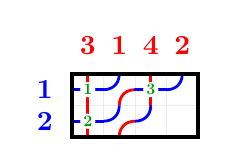
\begin{tikzpicture}[scale=0.4]
  \draw[lightgray, very thin, opacity=0.3] (0,2) -- (4,2);
  \draw[lightgray, very thin, opacity=0.3] (0,3) -- (4,3);
  \draw[lightgray, very thin, opacity=0.3] (0,4) -- (4,4);
  \draw[lightgray, very thin, opacity=0.3] (0,2) -- (0,4);
  \draw[lightgray, very thin, opacity=0.3] (1,2) -- (1,4);
  \draw[lightgray, very thin, opacity=0.3] (2,2) -- (2,4);
  \draw[lightgray, very thin, opacity=0.3] (3,2) -- (3,4);
  \draw[lightgray, very thin, opacity=0.3] (4,2) -- (4,4);
  \draw[blue, line width=1.0pt, line cap=round] (0,3.5) -- (1,3.5);
  \draw[red, line width=1.0pt, line cap=round] (0.5,3) -- (0.5,4);
  \draw[blue, line width=1.0pt] (1,3.5) .. controls (1.3,3.5) and (1.5,3.7) .. (1.5,4);
  \draw[red, line width=1.0pt] (1.5,3) .. controls (1.5,3.3) and (1.7,3.5) .. (2,3.5);
  \draw[blue, line width=1.0pt, line cap=round] (2,3.5) -- (3,3.5);
  \draw[red, line width=1.0pt, line cap=round] (2.5,3) -- (2.5,4);
  \draw[blue, line width=1.0pt] (3,3.5) .. controls (3.3,3.5) and (3.5,3.7) .. (3.5,4);
  \draw[blue, line width=1.0pt, line cap=round] (0,2.5) -- (1,2.5);
  \draw[red, line width=1.0pt, line cap=round] (0.5,2) -- (0.5,3);
  \draw[blue, line width=1.0pt] (1,2.5) .. controls (1.3,2.5) and (1.5,2.7) .. (1.5,3);
  \draw[red, line width=1.0pt] (1.5,2) .. controls (1.5,2.3) and (1.7,2.5) .. (2,2.5);
  \draw[blue, line width=1.0pt] (2,2.5) .. controls (2.3,2.5) and (2.5,2.7) .. (2.5,3);
  \node[font=\Large\bfseries, text=green!60!black, fill=white, inner sep=0.5pt, circle, transform shape] at (0.5,3.5) {1};
  \node[font=\Large\bfseries, text=green!60!black, fill=white, inner sep=0.5pt, circle, transform shape] at (2.5,3.5) {3};
  \node[font=\Large\bfseries, text=green!60!black, fill=white, inner sep=0.5pt, circle, transform shape] at (0.5,2.5) {2};
  \node[font=\bfseries, text=red, anchor=south] at (0.5,4.3) {3};
  \node[font=\bfseries, text=red, anchor=south] at (1.5,4.3) {1};
  \node[font=\bfseries, text=red, anchor=south] at (2.5,4.3) {4};
  \node[font=\bfseries, text=red, anchor=south] at (3.5,4.3) {2};
  \node[font=\bfseries, text=blue, anchor=east] at (-0.3,3.5) {1};
  \node[font=\bfseries, text=blue, anchor=east] at (-0.3,2.5) {2};
  \draw[black, line width=1.2000000000000002pt] (0,2) rectangle (4,4);
\end{tikzpicture}}}
  \diamond
  \vcenter{\hbox{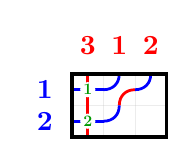
\begin{tikzpicture}[scale=0.4]
  \draw[lightgray, very thin, opacity=0.3] (0,1) -- (3,1);
  \draw[lightgray, very thin, opacity=0.3] (0,2) -- (3,2);
  \draw[lightgray, very thin, opacity=0.3] (0,3) -- (3,3);
  \draw[lightgray, very thin, opacity=0.3] (0,1) -- (0,3);
  \draw[lightgray, very thin, opacity=0.3] (1,1) -- (1,3);
  \draw[lightgray, very thin, opacity=0.3] (2,1) -- (2,3);
  \draw[lightgray, very thin, opacity=0.3] (3,1) -- (3,3);
  \draw[blue, line width=1.0pt, line cap=round] (0,2.5) -- (1,2.5);
  \draw[red, line width=1.0pt, line cap=round] (0.5,2) -- (0.5,3);
  \draw[blue, line width=1.0pt] (1,2.5) .. controls (1.3,2.5) and (1.5,2.7) .. (1.5,3);
  \draw[red, line width=1.0pt] (1.5,2) .. controls (1.5,2.3) and (1.7,2.5) .. (2,2.5);
  \draw[blue, line width=1.0pt] (2,2.5) .. controls (2.3,2.5) and (2.5,2.7) .. (2.5,3);
  \draw[blue, line width=1.0pt, line cap=round] (0,1.5) -- (1,1.5);
  \draw[red, line width=1.0pt, line cap=round] (0.5,1) -- (0.5,2);
  \draw[blue, line width=1.0pt] (1,1.5) .. controls (1.3,1.5) and (1.5,1.7) .. (1.5,2);
  \node[font=\Large\bfseries, text=green!60!black, fill=white, inner sep=0.5pt, circle, transform shape] at (0.5,2.5) {1};
  \node[font=\Large\bfseries, text=green!60!black, fill=white, inner sep=0.5pt, circle, transform shape] at (0.5,1.5) {2};
  \node[font=\bfseries, text=red, anchor=south] at (0.5,3.3) {3};
  \node[font=\bfseries, text=red, anchor=south] at (1.5,3.3) {1};
  \node[font=\bfseries, text=red, anchor=south] at (2.5,3.3) {2};
  \node[font=\bfseries, text=blue, anchor=east] at (-0.3,2.5) {1};
  \node[font=\bfseries, text=blue, anchor=east] at (-0.3,1.5) {2};
  \draw[black, line width=1.2000000000000002pt] (0,1) rectangle (3,3);
\end{tikzpicture}}}
  \\[1em]
  ={}& 
  \vcenter{\hbox{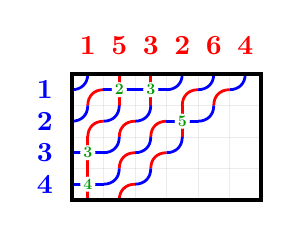
\begin{tikzpicture}[scale=0.4]
  \draw[lightgray, very thin, opacity=0.3] (0,2) -- (6,2);
  \draw[lightgray, very thin, opacity=0.3] (0,3) -- (6,3);
  \draw[lightgray, very thin, opacity=0.3] (0,4) -- (6,4);
  \draw[lightgray, very thin, opacity=0.3] (0,5) -- (6,5);
  \draw[lightgray, very thin, opacity=0.3] (0,6) -- (6,6);
  \draw[lightgray, very thin, opacity=0.3] (0,2) -- (0,6);
  \draw[lightgray, very thin, opacity=0.3] (1,2) -- (1,6);
  \draw[lightgray, very thin, opacity=0.3] (2,2) -- (2,6);
  \draw[lightgray, very thin, opacity=0.3] (3,2) -- (3,6);
  \draw[lightgray, very thin, opacity=0.3] (4,2) -- (4,6);
  \draw[lightgray, very thin, opacity=0.3] (5,2) -- (5,6);
  \draw[lightgray, very thin, opacity=0.3] (6,2) -- (6,6);
  \draw[blue, line width=1.0pt] (0,5.5) .. controls (0.3,5.5) and (0.5,5.7) .. (0.5,6);
  \draw[red, line width=1.0pt] (0.5,5) .. controls (0.5,5.3) and (0.7,5.5) .. (1,5.5);
  \draw[blue, line width=1.0pt, line cap=round] (1,5.5) -- (2,5.5);
  \draw[red, line width=1.0pt, line cap=round] (1.5,5) -- (1.5,6);
  \draw[blue, line width=1.0pt, line cap=round] (2,5.5) -- (3,5.5);
  \draw[red, line width=1.0pt, line cap=round] (2.5,5) -- (2.5,6);
  \draw[blue, line width=1.0pt] (3,5.5) .. controls (3.3,5.5) and (3.5,5.7) .. (3.5,6);
  \draw[red, line width=1.0pt] (3.5,5) .. controls (3.5,5.3) and (3.7,5.5) .. (4,5.5);
  \draw[blue, line width=1.0pt] (4,5.5) .. controls (4.3,5.5) and (4.5,5.7) .. (4.5,6);
  \draw[red, line width=1.0pt] (4.5,5) .. controls (4.5,5.3) and (4.7,5.5) .. (5,5.5);
  \draw[blue, line width=1.0pt] (5,5.5) .. controls (5.3,5.5) and (5.5,5.7) .. (5.5,6);
  \draw[blue, line width=1.0pt] (0,4.5) .. controls (0.3,4.5) and (0.5,4.7) .. (0.5,5);
  \draw[red, line width=1.0pt] (0.5,4) .. controls (0.5,4.3) and (0.7,4.5) .. (1,4.5);
  \draw[blue, line width=1.0pt] (1,4.5) .. controls (1.3,4.5) and (1.5,4.7) .. (1.5,5);
  \draw[red, line width=1.0pt] (1.5,4) .. controls (1.5,4.3) and (1.7,4.5) .. (2,4.5);
  \draw[blue, line width=1.0pt] (2,4.5) .. controls (2.3,4.5) and (2.5,4.7) .. (2.5,5);
  \draw[red, line width=1.0pt] (2.5,4) .. controls (2.5,4.3) and (2.7,4.5) .. (3,4.5);
  \draw[blue, line width=1.0pt, line cap=round] (3,4.5) -- (4,4.5);
  \draw[red, line width=1.0pt, line cap=round] (3.5,4) -- (3.5,5);
  \draw[blue, line width=1.0pt] (4,4.5) .. controls (4.3,4.5) and (4.5,4.7) .. (4.5,5);
  \draw[blue, line width=1.0pt, line cap=round] (0,3.5) -- (1,3.5);
  \draw[red, line width=1.0pt, line cap=round] (0.5,3) -- (0.5,4);
  \draw[blue, line width=1.0pt] (1,3.5) .. controls (1.3,3.5) and (1.5,3.7) .. (1.5,4);
  \draw[red, line width=1.0pt] (1.5,3) .. controls (1.5,3.3) and (1.7,3.5) .. (2,3.5);
  \draw[blue, line width=1.0pt] (2,3.5) .. controls (2.3,3.5) and (2.5,3.7) .. (2.5,4);
  \draw[red, line width=1.0pt] (2.5,3) .. controls (2.5,3.3) and (2.7,3.5) .. (3,3.5);
  \draw[blue, line width=1.0pt] (3,3.5) .. controls (3.3,3.5) and (3.5,3.7) .. (3.5,4);
  \draw[blue, line width=1.0pt, line cap=round] (0,2.5) -- (1,2.5);
  \draw[red, line width=1.0pt, line cap=round] (0.5,2) -- (0.5,3);
  \draw[blue, line width=1.0pt] (1,2.5) .. controls (1.3,2.5) and (1.5,2.7) .. (1.5,3);
  \draw[red, line width=1.0pt] (1.5,2) .. controls (1.5,2.3) and (1.7,2.5) .. (2,2.5);
  \draw[blue, line width=1.0pt] (2,2.5) .. controls (2.3,2.5) and (2.5,2.7) .. (2.5,3);
  \node[font=\Large\bfseries, text=green!60!black, fill=white, inner sep=0.5pt, circle, transform shape] at (3.5,4.5) {5};
  \node[font=\Large\bfseries, text=green!60!black, fill=white, inner sep=0.5pt, circle, transform shape] at (1.5,5.5) {2};
  \node[font=\Large\bfseries, text=green!60!black, fill=white, inner sep=0.5pt, circle, transform shape] at (0.5,2.5) {4};
  \node[font=\Large\bfseries, text=green!60!black, fill=white, inner sep=0.5pt, circle, transform shape] at (0.5,3.5) {3};
  \node[font=\Large\bfseries, text=green!60!black, fill=white, inner sep=0.5pt, circle, transform shape] at (2.5,5.5) {3};
  \node[font=\bfseries, text=red, anchor=south] at (0.5,6.3) {1};
  \node[font=\bfseries, text=red, anchor=south] at (1.5,6.3) {5};
  \node[font=\bfseries, text=red, anchor=south] at (2.5,6.3) {3};
  \node[font=\bfseries, text=red, anchor=south] at (3.5,6.3) {2};
  \node[font=\bfseries, text=red, anchor=south] at (4.5,6.3) {6};
  \node[font=\bfseries, text=red, anchor=south] at (5.5,6.3) {4};
  \node[font=\bfseries, text=blue, anchor=east] at (-0.3,5.5) {1};
  \node[font=\bfseries, text=blue, anchor=east] at (-0.3,4.5) {2};
  \node[font=\bfseries, text=blue, anchor=east] at (-0.3,3.5) {3};
  \node[font=\bfseries, text=blue, anchor=east] at (-0.3,2.5) {4};
  \draw[black, line width=1.2000000000000002pt] (0,2) rectangle (6,6);
\end{tikzpicture}}}
  +
  \vcenter{\hbox{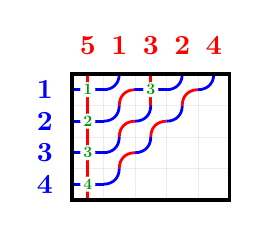
\begin{tikzpicture}[scale=0.4]
  \draw[lightgray, very thin, opacity=0.3] (0,1) -- (5,1);
  \draw[lightgray, very thin, opacity=0.3] (0,2) -- (5,2);
  \draw[lightgray, very thin, opacity=0.3] (0,3) -- (5,3);
  \draw[lightgray, very thin, opacity=0.3] (0,4) -- (5,4);
  \draw[lightgray, very thin, opacity=0.3] (0,5) -- (5,5);
  \draw[lightgray, very thin, opacity=0.3] (0,1) -- (0,5);
  \draw[lightgray, very thin, opacity=0.3] (1,1) -- (1,5);
  \draw[lightgray, very thin, opacity=0.3] (2,1) -- (2,5);
  \draw[lightgray, very thin, opacity=0.3] (3,1) -- (3,5);
  \draw[lightgray, very thin, opacity=0.3] (4,1) -- (4,5);
  \draw[lightgray, very thin, opacity=0.3] (5,1) -- (5,5);
  \draw[blue, line width=1.0pt, line cap=round] (0,4.5) -- (1,4.5);
  \draw[red, line width=1.0pt, line cap=round] (0.5,4) -- (0.5,5);
  \draw[blue, line width=1.0pt] (1,4.5) .. controls (1.3,4.5) and (1.5,4.7) .. (1.5,5);
  \draw[red, line width=1.0pt] (1.5,4) .. controls (1.5,4.3) and (1.7,4.5) .. (2,4.5);
  \draw[blue, line width=1.0pt, line cap=round] (2,4.5) -- (3,4.5);
  \draw[red, line width=1.0pt, line cap=round] (2.5,4) -- (2.5,5);
  \draw[blue, line width=1.0pt] (3,4.5) .. controls (3.3,4.5) and (3.5,4.7) .. (3.5,5);
  \draw[red, line width=1.0pt] (3.5,4) .. controls (3.5,4.3) and (3.7,4.5) .. (4,4.5);
  \draw[blue, line width=1.0pt] (4,4.5) .. controls (4.3,4.5) and (4.5,4.7) .. (4.5,5);
  \draw[blue, line width=1.0pt, line cap=round] (0,3.5) -- (1,3.5);
  \draw[red, line width=1.0pt, line cap=round] (0.5,3) -- (0.5,4);
  \draw[blue, line width=1.0pt] (1,3.5) .. controls (1.3,3.5) and (1.5,3.7) .. (1.5,4);
  \draw[red, line width=1.0pt] (1.5,3) .. controls (1.5,3.3) and (1.7,3.5) .. (2,3.5);
  \draw[blue, line width=1.0pt] (2,3.5) .. controls (2.3,3.5) and (2.5,3.7) .. (2.5,4);
  \draw[red, line width=1.0pt] (2.5,3) .. controls (2.5,3.3) and (2.7,3.5) .. (3,3.5);
  \draw[blue, line width=1.0pt] (3,3.5) .. controls (3.3,3.5) and (3.5,3.7) .. (3.5,4);
  \draw[blue, line width=1.0pt, line cap=round] (0,2.5) -- (1,2.5);
  \draw[red, line width=1.0pt, line cap=round] (0.5,2) -- (0.5,3);
  \draw[blue, line width=1.0pt] (1,2.5) .. controls (1.3,2.5) and (1.5,2.7) .. (1.5,3);
  \draw[red, line width=1.0pt] (1.5,2) .. controls (1.5,2.3) and (1.7,2.5) .. (2,2.5);
  \draw[blue, line width=1.0pt] (2,2.5) .. controls (2.3,2.5) and (2.5,2.7) .. (2.5,3);
  \draw[blue, line width=1.0pt, line cap=round] (0,1.5) -- (1,1.5);
  \draw[red, line width=1.0pt, line cap=round] (0.5,1) -- (0.5,2);
  \draw[blue, line width=1.0pt] (1,1.5) .. controls (1.3,1.5) and (1.5,1.7) .. (1.5,2);
  \node[font=\Large\bfseries, text=green!60!black, fill=white, inner sep=0.5pt, circle, transform shape] at (0.5,3.5) {2};
  \node[font=\Large\bfseries, text=green!60!black, fill=white, inner sep=0.5pt, circle, transform shape] at (0.5,1.5) {4};
  \node[font=\Large\bfseries, text=green!60!black, fill=white, inner sep=0.5pt, circle, transform shape] at (0.5,2.5) {3};
  \node[font=\Large\bfseries, text=green!60!black, fill=white, inner sep=0.5pt, circle, transform shape] at (0.5,4.5) {1};
  \node[font=\Large\bfseries, text=green!60!black, fill=white, inner sep=0.5pt, circle, transform shape] at (2.5,4.5) {3};
  \node[font=\bfseries, text=red, anchor=south] at (0.5,5.3) {5};
  \node[font=\bfseries, text=red, anchor=south] at (1.5,5.3) {1};
  \node[font=\bfseries, text=red, anchor=south] at (2.5,5.3) {3};
  \node[font=\bfseries, text=red, anchor=south] at (3.5,5.3) {2};
  \node[font=\bfseries, text=red, anchor=south] at (4.5,5.3) {4};
  \node[font=\bfseries, text=blue, anchor=east] at (-0.3,4.5) {1};
  \node[font=\bfseries, text=blue, anchor=east] at (-0.3,3.5) {2};
  \node[font=\bfseries, text=blue, anchor=east] at (-0.3,2.5) {3};
  \node[font=\bfseries, text=blue, anchor=east] at (-0.3,1.5) {4};
  \draw[black, line width=1.2000000000000002pt] (0,1) rectangle (5,5);
\end{tikzpicture}}}
  +
  \vcenter{\hbox{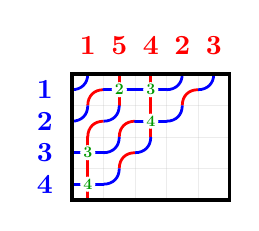
\begin{tikzpicture}[scale=0.4]
  \draw[lightgray, very thin, opacity=0.3] (0,1) -- (5,1);
  \draw[lightgray, very thin, opacity=0.3] (0,2) -- (5,2);
  \draw[lightgray, very thin, opacity=0.3] (0,3) -- (5,3);
  \draw[lightgray, very thin, opacity=0.3] (0,4) -- (5,4);
  \draw[lightgray, very thin, opacity=0.3] (0,5) -- (5,5);
  \draw[lightgray, very thin, opacity=0.3] (0,1) -- (0,5);
  \draw[lightgray, very thin, opacity=0.3] (1,1) -- (1,5);
  \draw[lightgray, very thin, opacity=0.3] (2,1) -- (2,5);
  \draw[lightgray, very thin, opacity=0.3] (3,1) -- (3,5);
  \draw[lightgray, very thin, opacity=0.3] (4,1) -- (4,5);
  \draw[lightgray, very thin, opacity=0.3] (5,1) -- (5,5);
  \draw[blue, line width=1.0pt] (0,4.5) .. controls (0.3,4.5) and (0.5,4.7) .. (0.5,5);
  \draw[red, line width=1.0pt] (0.5,4) .. controls (0.5,4.3) and (0.7,4.5) .. (1,4.5);
  \draw[blue, line width=1.0pt, line cap=round] (1,4.5) -- (2,4.5);
  \draw[red, line width=1.0pt, line cap=round] (1.5,4) -- (1.5,5);
  \draw[blue, line width=1.0pt, line cap=round] (2,4.5) -- (3,4.5);
  \draw[red, line width=1.0pt, line cap=round] (2.5,4) -- (2.5,5);
  \draw[blue, line width=1.0pt] (3,4.5) .. controls (3.3,4.5) and (3.5,4.7) .. (3.5,5);
  \draw[red, line width=1.0pt] (3.5,4) .. controls (3.5,4.3) and (3.7,4.5) .. (4,4.5);
  \draw[blue, line width=1.0pt] (4,4.5) .. controls (4.3,4.5) and (4.5,4.7) .. (4.5,5);
  \draw[blue, line width=1.0pt] (0,3.5) .. controls (0.3,3.5) and (0.5,3.7) .. (0.5,4);
  \draw[red, line width=1.0pt] (0.5,3) .. controls (0.5,3.3) and (0.7,3.5) .. (1,3.5);
  \draw[blue, line width=1.0pt] (1,3.5) .. controls (1.3,3.5) and (1.5,3.7) .. (1.5,4);
  \draw[red, line width=1.0pt] (1.5,3) .. controls (1.5,3.3) and (1.7,3.5) .. (2,3.5);
  \draw[blue, line width=1.0pt, line cap=round] (2,3.5) -- (3,3.5);
  \draw[red, line width=1.0pt, line cap=round] (2.5,3) -- (2.5,4);
  \draw[blue, line width=1.0pt] (3,3.5) .. controls (3.3,3.5) and (3.5,3.7) .. (3.5,4);
  \draw[blue, line width=1.0pt, line cap=round] (0,2.5) -- (1,2.5);
  \draw[red, line width=1.0pt, line cap=round] (0.5,2) -- (0.5,3);
  \draw[blue, line width=1.0pt] (1,2.5) .. controls (1.3,2.5) and (1.5,2.7) .. (1.5,3);
  \draw[red, line width=1.0pt] (1.5,2) .. controls (1.5,2.3) and (1.7,2.5) .. (2,2.5);
  \draw[blue, line width=1.0pt] (2,2.5) .. controls (2.3,2.5) and (2.5,2.7) .. (2.5,3);
  \draw[blue, line width=1.0pt, line cap=round] (0,1.5) -- (1,1.5);
  \draw[red, line width=1.0pt, line cap=round] (0.5,1) -- (0.5,2);
  \draw[blue, line width=1.0pt] (1,1.5) .. controls (1.3,1.5) and (1.5,1.7) .. (1.5,2);
  \node[font=\Large\bfseries, text=green!60!black, fill=white, inner sep=0.5pt, circle, transform shape] at (1.5,4.5) {2};
  \node[font=\Large\bfseries, text=green!60!black, fill=white, inner sep=0.5pt, circle, transform shape] at (0.5,1.5) {4};
  \node[font=\Large\bfseries, text=green!60!black, fill=white, inner sep=0.5pt, circle, transform shape] at (0.5,2.5) {3};
  \node[font=\Large\bfseries, text=green!60!black, fill=white, inner sep=0.5pt, circle, transform shape] at (2.5,3.5) {4};
  \node[font=\Large\bfseries, text=green!60!black, fill=white, inner sep=0.5pt, circle, transform shape] at (2.5,4.5) {3};
  \node[font=\bfseries, text=red, anchor=south] at (0.5,5.3) {1};
  \node[font=\bfseries, text=red, anchor=south] at (1.5,5.3) {5};
  \node[font=\bfseries, text=red, anchor=south] at (2.5,5.3) {4};
  \node[font=\bfseries, text=red, anchor=south] at (3.5,5.3) {2};
  \node[font=\bfseries, text=red, anchor=south] at (4.5,5.3) {3};
  \node[font=\bfseries, text=blue, anchor=east] at (-0.3,4.5) {1};
  \node[font=\bfseries, text=blue, anchor=east] at (-0.3,3.5) {2};
  \node[font=\bfseries, text=blue, anchor=east] at (-0.3,2.5) {3};
  \node[font=\bfseries, text=blue, anchor=east] at (-0.3,1.5) {4};
  \draw[black, line width=1.2000000000000002pt] (0,1) rectangle (5,5);
\end{tikzpicture}}}
  \\[1em]
  + & 
  \vcenter{\hbox{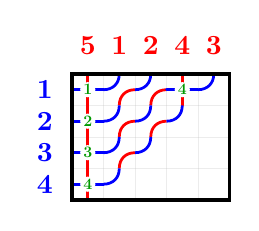
\begin{tikzpicture}[scale=0.4]
  \draw[lightgray, very thin, opacity=0.3] (0,1) -- (5,1);
  \draw[lightgray, very thin, opacity=0.3] (0,2) -- (5,2);
  \draw[lightgray, very thin, opacity=0.3] (0,3) -- (5,3);
  \draw[lightgray, very thin, opacity=0.3] (0,4) -- (5,4);
  \draw[lightgray, very thin, opacity=0.3] (0,5) -- (5,5);
  \draw[lightgray, very thin, opacity=0.3] (0,1) -- (0,5);
  \draw[lightgray, very thin, opacity=0.3] (1,1) -- (1,5);
  \draw[lightgray, very thin, opacity=0.3] (2,1) -- (2,5);
  \draw[lightgray, very thin, opacity=0.3] (3,1) -- (3,5);
  \draw[lightgray, very thin, opacity=0.3] (4,1) -- (4,5);
  \draw[lightgray, very thin, opacity=0.3] (5,1) -- (5,5);
  \draw[blue, line width=1.0pt, line cap=round] (0,4.5) -- (1,4.5);
  \draw[red, line width=1.0pt, line cap=round] (0.5,4) -- (0.5,5);
  \draw[blue, line width=1.0pt] (1,4.5) .. controls (1.3,4.5) and (1.5,4.7) .. (1.5,5);
  \draw[red, line width=1.0pt] (1.5,4) .. controls (1.5,4.3) and (1.7,4.5) .. (2,4.5);
  \draw[blue, line width=1.0pt] (2,4.5) .. controls (2.3,4.5) and (2.5,4.7) .. (2.5,5);
  \draw[red, line width=1.0pt] (2.5,4) .. controls (2.5,4.3) and (2.7,4.5) .. (3,4.5);
  \draw[blue, line width=1.0pt, line cap=round] (3,4.5) -- (4,4.5);
  \draw[red, line width=1.0pt, line cap=round] (3.5,4) -- (3.5,5);
  \draw[blue, line width=1.0pt] (4,4.5) .. controls (4.3,4.5) and (4.5,4.7) .. (4.5,5);
  \draw[blue, line width=1.0pt, line cap=round] (0,3.5) -- (1,3.5);
  \draw[red, line width=1.0pt, line cap=round] (0.5,3) -- (0.5,4);
  \draw[blue, line width=1.0pt] (1,3.5) .. controls (1.3,3.5) and (1.5,3.7) .. (1.5,4);
  \draw[red, line width=1.0pt] (1.5,3) .. controls (1.5,3.3) and (1.7,3.5) .. (2,3.5);
  \draw[blue, line width=1.0pt] (2,3.5) .. controls (2.3,3.5) and (2.5,3.7) .. (2.5,4);
  \draw[red, line width=1.0pt] (2.5,3) .. controls (2.5,3.3) and (2.7,3.5) .. (3,3.5);
  \draw[blue, line width=1.0pt] (3,3.5) .. controls (3.3,3.5) and (3.5,3.7) .. (3.5,4);
  \draw[blue, line width=1.0pt, line cap=round] (0,2.5) -- (1,2.5);
  \draw[red, line width=1.0pt, line cap=round] (0.5,2) -- (0.5,3);
  \draw[blue, line width=1.0pt] (1,2.5) .. controls (1.3,2.5) and (1.5,2.7) .. (1.5,3);
  \draw[red, line width=1.0pt] (1.5,2) .. controls (1.5,2.3) and (1.7,2.5) .. (2,2.5);
  \draw[blue, line width=1.0pt] (2,2.5) .. controls (2.3,2.5) and (2.5,2.7) .. (2.5,3);
  \draw[blue, line width=1.0pt, line cap=round] (0,1.5) -- (1,1.5);
  \draw[red, line width=1.0pt, line cap=round] (0.5,1) -- (0.5,2);
  \draw[blue, line width=1.0pt] (1,1.5) .. controls (1.3,1.5) and (1.5,1.7) .. (1.5,2);
  \node[font=\Large\bfseries, text=green!60!black, fill=white, inner sep=0.5pt, circle, transform shape] at (0.5,3.5) {2};
  \node[font=\Large\bfseries, text=green!60!black, fill=white, inner sep=0.5pt, circle, transform shape] at (0.5,2.5) {3};
  \node[font=\Large\bfseries, text=green!60!black, fill=white, inner sep=0.5pt, circle, transform shape] at (0.5,4.5) {1};
  \node[font=\Large\bfseries, text=green!60!black, fill=white, inner sep=0.5pt, circle, transform shape] at (3.5,4.5) {4};
  \node[font=\Large\bfseries, text=green!60!black, fill=white, inner sep=0.5pt, circle, transform shape] at (0.5,1.5) {4};
  \node[font=\bfseries, text=red, anchor=south] at (0.5,5.3) {5};
  \node[font=\bfseries, text=red, anchor=south] at (1.5,5.3) {1};
  \node[font=\bfseries, text=red, anchor=south] at (2.5,5.3) {2};
  \node[font=\bfseries, text=red, anchor=south] at (3.5,5.3) {4};
  \node[font=\bfseries, text=red, anchor=south] at (4.5,5.3) {3};
  \node[font=\bfseries, text=blue, anchor=east] at (-0.3,4.5) {1};
  \node[font=\bfseries, text=blue, anchor=east] at (-0.3,3.5) {2};
  \node[font=\bfseries, text=blue, anchor=east] at (-0.3,2.5) {3};
  \node[font=\bfseries, text=blue, anchor=east] at (-0.3,1.5) {4};
  \draw[black, line width=1.2000000000000002pt] (0,1) rectangle (5,5);
\end{tikzpicture}}}
  +
  \vcenter{\hbox{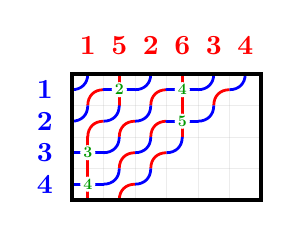
\begin{tikzpicture}[scale=0.4]
  \draw[lightgray, very thin, opacity=0.3] (0,2) -- (6,2);
  \draw[lightgray, very thin, opacity=0.3] (0,3) -- (6,3);
  \draw[lightgray, very thin, opacity=0.3] (0,4) -- (6,4);
  \draw[lightgray, very thin, opacity=0.3] (0,5) -- (6,5);
  \draw[lightgray, very thin, opacity=0.3] (0,6) -- (6,6);
  \draw[lightgray, very thin, opacity=0.3] (0,2) -- (0,6);
  \draw[lightgray, very thin, opacity=0.3] (1,2) -- (1,6);
  \draw[lightgray, very thin, opacity=0.3] (2,2) -- (2,6);
  \draw[lightgray, very thin, opacity=0.3] (3,2) -- (3,6);
  \draw[lightgray, very thin, opacity=0.3] (4,2) -- (4,6);
  \draw[lightgray, very thin, opacity=0.3] (5,2) -- (5,6);
  \draw[lightgray, very thin, opacity=0.3] (6,2) -- (6,6);
  \draw[blue, line width=1.0pt] (0,5.5) .. controls (0.3,5.5) and (0.5,5.7) .. (0.5,6);
  \draw[red, line width=1.0pt] (0.5,5) .. controls (0.5,5.3) and (0.7,5.5) .. (1,5.5);
  \draw[blue, line width=1.0pt, line cap=round] (1,5.5) -- (2,5.5);
  \draw[red, line width=1.0pt, line cap=round] (1.5,5) -- (1.5,6);
  \draw[blue, line width=1.0pt] (2,5.5) .. controls (2.3,5.5) and (2.5,5.7) .. (2.5,6);
  \draw[red, line width=1.0pt] (2.5,5) .. controls (2.5,5.3) and (2.7,5.5) .. (3,5.5);
  \draw[blue, line width=1.0pt, line cap=round] (3,5.5) -- (4,5.5);
  \draw[red, line width=1.0pt, line cap=round] (3.5,5) -- (3.5,6);
  \draw[blue, line width=1.0pt] (4,5.5) .. controls (4.3,5.5) and (4.5,5.7) .. (4.5,6);
  \draw[red, line width=1.0pt] (4.5,5) .. controls (4.5,5.3) and (4.7,5.5) .. (5,5.5);
  \draw[blue, line width=1.0pt] (5,5.5) .. controls (5.3,5.5) and (5.5,5.7) .. (5.5,6);
  \draw[blue, line width=1.0pt] (0,4.5) .. controls (0.3,4.5) and (0.5,4.7) .. (0.5,5);
  \draw[red, line width=1.0pt] (0.5,4) .. controls (0.5,4.3) and (0.7,4.5) .. (1,4.5);
  \draw[blue, line width=1.0pt] (1,4.5) .. controls (1.3,4.5) and (1.5,4.7) .. (1.5,5);
  \draw[red, line width=1.0pt] (1.5,4) .. controls (1.5,4.3) and (1.7,4.5) .. (2,4.5);
  \draw[blue, line width=1.0pt] (2,4.5) .. controls (2.3,4.5) and (2.5,4.7) .. (2.5,5);
  \draw[red, line width=1.0pt] (2.5,4) .. controls (2.5,4.3) and (2.7,4.5) .. (3,4.5);
  \draw[blue, line width=1.0pt, line cap=round] (3,4.5) -- (4,4.5);
  \draw[red, line width=1.0pt, line cap=round] (3.5,4) -- (3.5,5);
  \draw[blue, line width=1.0pt] (4,4.5) .. controls (4.3,4.5) and (4.5,4.7) .. (4.5,5);
  \draw[blue, line width=1.0pt, line cap=round] (0,3.5) -- (1,3.5);
  \draw[red, line width=1.0pt, line cap=round] (0.5,3) -- (0.5,4);
  \draw[blue, line width=1.0pt] (1,3.5) .. controls (1.3,3.5) and (1.5,3.7) .. (1.5,4);
  \draw[red, line width=1.0pt] (1.5,3) .. controls (1.5,3.3) and (1.7,3.5) .. (2,3.5);
  \draw[blue, line width=1.0pt] (2,3.5) .. controls (2.3,3.5) and (2.5,3.7) .. (2.5,4);
  \draw[red, line width=1.0pt] (2.5,3) .. controls (2.5,3.3) and (2.7,3.5) .. (3,3.5);
  \draw[blue, line width=1.0pt] (3,3.5) .. controls (3.3,3.5) and (3.5,3.7) .. (3.5,4);
  \draw[blue, line width=1.0pt, line cap=round] (0,2.5) -- (1,2.5);
  \draw[red, line width=1.0pt, line cap=round] (0.5,2) -- (0.5,3);
  \draw[blue, line width=1.0pt] (1,2.5) .. controls (1.3,2.5) and (1.5,2.7) .. (1.5,3);
  \draw[red, line width=1.0pt] (1.5,2) .. controls (1.5,2.3) and (1.7,2.5) .. (2,2.5);
  \draw[blue, line width=1.0pt] (2,2.5) .. controls (2.3,2.5) and (2.5,2.7) .. (2.5,3);
  \node[font=\Large\bfseries, text=green!60!black, fill=white, inner sep=0.5pt, circle, transform shape] at (3.5,4.5) {5};
  \node[font=\Large\bfseries, text=green!60!black, fill=white, inner sep=0.5pt, circle, transform shape] at (1.5,5.5) {2};
  \node[font=\Large\bfseries, text=green!60!black, fill=white, inner sep=0.5pt, circle, transform shape] at (0.5,3.5) {3};
  \node[font=\Large\bfseries, text=green!60!black, fill=white, inner sep=0.5pt, circle, transform shape] at (3.5,5.5) {4};
  \node[font=\Large\bfseries, text=green!60!black, fill=white, inner sep=0.5pt, circle, transform shape] at (0.5,2.5) {4};
  \node[font=\bfseries, text=red, anchor=south] at (0.5,6.3) {1};
  \node[font=\bfseries, text=red, anchor=south] at (1.5,6.3) {5};
  \node[font=\bfseries, text=red, anchor=south] at (2.5,6.3) {2};
  \node[font=\bfseries, text=red, anchor=south] at (3.5,6.3) {6};
  \node[font=\bfseries, text=red, anchor=south] at (4.5,6.3) {3};
  \node[font=\bfseries, text=red, anchor=south] at (5.5,6.3) {4};
  \node[font=\bfseries, text=blue, anchor=east] at (-0.3,5.5) {1};
  \node[font=\bfseries, text=blue, anchor=east] at (-0.3,4.5) {2};
  \node[font=\bfseries, text=blue, anchor=east] at (-0.3,3.5) {3};
  \node[font=\bfseries, text=blue, anchor=east] at (-0.3,2.5) {4};
  \draw[black, line width=1.2000000000000002pt] (0,2) rectangle (6,6);
\end{tikzpicture}}}
  +
  \vcenter{\hbox{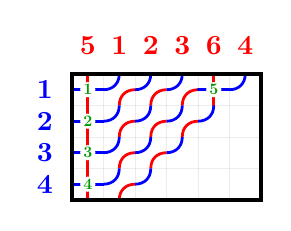
\begin{tikzpicture}[scale=0.4]
  \draw[lightgray, very thin, opacity=0.3] (0,2) -- (6,2);
  \draw[lightgray, very thin, opacity=0.3] (0,3) -- (6,3);
  \draw[lightgray, very thin, opacity=0.3] (0,4) -- (6,4);
  \draw[lightgray, very thin, opacity=0.3] (0,5) -- (6,5);
  \draw[lightgray, very thin, opacity=0.3] (0,6) -- (6,6);
  \draw[lightgray, very thin, opacity=0.3] (0,2) -- (0,6);
  \draw[lightgray, very thin, opacity=0.3] (1,2) -- (1,6);
  \draw[lightgray, very thin, opacity=0.3] (2,2) -- (2,6);
  \draw[lightgray, very thin, opacity=0.3] (3,2) -- (3,6);
  \draw[lightgray, very thin, opacity=0.3] (4,2) -- (4,6);
  \draw[lightgray, very thin, opacity=0.3] (5,2) -- (5,6);
  \draw[lightgray, very thin, opacity=0.3] (6,2) -- (6,6);
  \draw[blue, line width=1.0pt, line cap=round] (0,5.5) -- (1,5.5);
  \draw[red, line width=1.0pt, line cap=round] (0.5,5) -- (0.5,6);
  \draw[blue, line width=1.0pt] (1,5.5) .. controls (1.3,5.5) and (1.5,5.7) .. (1.5,6);
  \draw[red, line width=1.0pt] (1.5,5) .. controls (1.5,5.3) and (1.7,5.5) .. (2,5.5);
  \draw[blue, line width=1.0pt] (2,5.5) .. controls (2.3,5.5) and (2.5,5.7) .. (2.5,6);
  \draw[red, line width=1.0pt] (2.5,5) .. controls (2.5,5.3) and (2.7,5.5) .. (3,5.5);
  \draw[blue, line width=1.0pt] (3,5.5) .. controls (3.3,5.5) and (3.5,5.7) .. (3.5,6);
  \draw[red, line width=1.0pt] (3.5,5) .. controls (3.5,5.3) and (3.7,5.5) .. (4,5.5);
  \draw[blue, line width=1.0pt, line cap=round] (4,5.5) -- (5,5.5);
  \draw[red, line width=1.0pt, line cap=round] (4.5,5) -- (4.5,6);
  \draw[blue, line width=1.0pt] (5,5.5) .. controls (5.3,5.5) and (5.5,5.7) .. (5.5,6);
  \draw[blue, line width=1.0pt, line cap=round] (0,4.5) -- (1,4.5);
  \draw[red, line width=1.0pt, line cap=round] (0.5,4) -- (0.5,5);
  \draw[blue, line width=1.0pt] (1,4.5) .. controls (1.3,4.5) and (1.5,4.7) .. (1.5,5);
  \draw[red, line width=1.0pt] (1.5,4) .. controls (1.5,4.3) and (1.7,4.5) .. (2,4.5);
  \draw[blue, line width=1.0pt] (2,4.5) .. controls (2.3,4.5) and (2.5,4.7) .. (2.5,5);
  \draw[red, line width=1.0pt] (2.5,4) .. controls (2.5,4.3) and (2.7,4.5) .. (3,4.5);
  \draw[blue, line width=1.0pt] (3,4.5) .. controls (3.3,4.5) and (3.5,4.7) .. (3.5,5);
  \draw[red, line width=1.0pt] (3.5,4) .. controls (3.5,4.3) and (3.7,4.5) .. (4,4.5);
  \draw[blue, line width=1.0pt] (4,4.5) .. controls (4.3,4.5) and (4.5,4.7) .. (4.5,5);
  \draw[blue, line width=1.0pt, line cap=round] (0,3.5) -- (1,3.5);
  \draw[red, line width=1.0pt, line cap=round] (0.5,3) -- (0.5,4);
  \draw[blue, line width=1.0pt] (1,3.5) .. controls (1.3,3.5) and (1.5,3.7) .. (1.5,4);
  \draw[red, line width=1.0pt] (1.5,3) .. controls (1.5,3.3) and (1.7,3.5) .. (2,3.5);
  \draw[blue, line width=1.0pt] (2,3.5) .. controls (2.3,3.5) and (2.5,3.7) .. (2.5,4);
  \draw[red, line width=1.0pt] (2.5,3) .. controls (2.5,3.3) and (2.7,3.5) .. (3,3.5);
  \draw[blue, line width=1.0pt] (3,3.5) .. controls (3.3,3.5) and (3.5,3.7) .. (3.5,4);
  \draw[blue, line width=1.0pt, line cap=round] (0,2.5) -- (1,2.5);
  \draw[red, line width=1.0pt, line cap=round] (0.5,2) -- (0.5,3);
  \draw[blue, line width=1.0pt] (1,2.5) .. controls (1.3,2.5) and (1.5,2.7) .. (1.5,3);
  \draw[red, line width=1.0pt] (1.5,2) .. controls (1.5,2.3) and (1.7,2.5) .. (2,2.5);
  \draw[blue, line width=1.0pt] (2,2.5) .. controls (2.3,2.5) and (2.5,2.7) .. (2.5,3);
  \node[font=\Large\bfseries, text=green!60!black, fill=white, inner sep=0.5pt, circle, transform shape] at (0.5,4.5) {2};
  \node[font=\Large\bfseries, text=green!60!black, fill=white, inner sep=0.5pt, circle, transform shape] at (4.5,5.5) {5};
  \node[font=\Large\bfseries, text=green!60!black, fill=white, inner sep=0.5pt, circle, transform shape] at (0.5,3.5) {3};
  \node[font=\Large\bfseries, text=green!60!black, fill=white, inner sep=0.5pt, circle, transform shape] at (0.5,5.5) {1};
  \node[font=\Large\bfseries, text=green!60!black, fill=white, inner sep=0.5pt, circle, transform shape] at (0.5,2.5) {4};
  \node[font=\bfseries, text=red, anchor=south] at (0.5,6.3) {5};
  \node[font=\bfseries, text=red, anchor=south] at (1.5,6.3) {1};
  \node[font=\bfseries, text=red, anchor=south] at (2.5,6.3) {2};
  \node[font=\bfseries, text=red, anchor=south] at (3.5,6.3) {3};
  \node[font=\bfseries, text=red, anchor=south] at (4.5,6.3) {6};
  \node[font=\bfseries, text=red, anchor=south] at (5.5,6.3) {4};
  \node[font=\bfseries, text=blue, anchor=east] at (-0.3,5.5) {1};
  \node[font=\bfseries, text=blue, anchor=east] at (-0.3,4.5) {2};
  \node[font=\bfseries, text=blue, anchor=east] at (-0.3,3.5) {3};
  \node[font=\bfseries, text=blue, anchor=east] at (-0.3,2.5) {4};
  \draw[black, line width=1.2000000000000002pt] (0,2) rectangle (6,6);
\end{tikzpicture}}}
  \\[1em]
  + & 
  \vcenter{\hbox{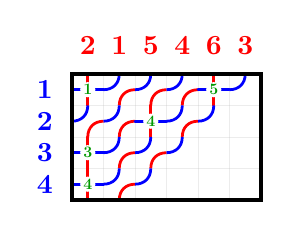
\begin{tikzpicture}[scale=0.4]
  \draw[lightgray, very thin, opacity=0.3] (0,2) -- (6,2);
  \draw[lightgray, very thin, opacity=0.3] (0,3) -- (6,3);
  \draw[lightgray, very thin, opacity=0.3] (0,4) -- (6,4);
  \draw[lightgray, very thin, opacity=0.3] (0,5) -- (6,5);
  \draw[lightgray, very thin, opacity=0.3] (0,6) -- (6,6);
  \draw[lightgray, very thin, opacity=0.3] (0,2) -- (0,6);
  \draw[lightgray, very thin, opacity=0.3] (1,2) -- (1,6);
  \draw[lightgray, very thin, opacity=0.3] (2,2) -- (2,6);
  \draw[lightgray, very thin, opacity=0.3] (3,2) -- (3,6);
  \draw[lightgray, very thin, opacity=0.3] (4,2) -- (4,6);
  \draw[lightgray, very thin, opacity=0.3] (5,2) -- (5,6);
  \draw[lightgray, very thin, opacity=0.3] (6,2) -- (6,6);
  \draw[blue, line width=1.0pt, line cap=round] (0,5.5) -- (1,5.5);
  \draw[red, line width=1.0pt, line cap=round] (0.5,5) -- (0.5,6);
  \draw[blue, line width=1.0pt] (1,5.5) .. controls (1.3,5.5) and (1.5,5.7) .. (1.5,6);
  \draw[red, line width=1.0pt] (1.5,5) .. controls (1.5,5.3) and (1.7,5.5) .. (2,5.5);
  \draw[blue, line width=1.0pt] (2,5.5) .. controls (2.3,5.5) and (2.5,5.7) .. (2.5,6);
  \draw[red, line width=1.0pt] (2.5,5) .. controls (2.5,5.3) and (2.7,5.5) .. (3,5.5);
  \draw[blue, line width=1.0pt] (3,5.5) .. controls (3.3,5.5) and (3.5,5.7) .. (3.5,6);
  \draw[red, line width=1.0pt] (3.5,5) .. controls (3.5,5.3) and (3.7,5.5) .. (4,5.5);
  \draw[blue, line width=1.0pt, line cap=round] (4,5.5) -- (5,5.5);
  \draw[red, line width=1.0pt, line cap=round] (4.5,5) -- (4.5,6);
  \draw[blue, line width=1.0pt] (5,5.5) .. controls (5.3,5.5) and (5.5,5.7) .. (5.5,6);
  \draw[blue, line width=1.0pt] (0,4.5) .. controls (0.3,4.5) and (0.5,4.7) .. (0.5,5);
  \draw[red, line width=1.0pt] (0.5,4) .. controls (0.5,4.3) and (0.7,4.5) .. (1,4.5);
  \draw[blue, line width=1.0pt] (1,4.5) .. controls (1.3,4.5) and (1.5,4.7) .. (1.5,5);
  \draw[red, line width=1.0pt] (1.5,4) .. controls (1.5,4.3) and (1.7,4.5) .. (2,4.5);
  \draw[blue, line width=1.0pt, line cap=round] (2,4.5) -- (3,4.5);
  \draw[red, line width=1.0pt, line cap=round] (2.5,4) -- (2.5,5);
  \draw[blue, line width=1.0pt] (3,4.5) .. controls (3.3,4.5) and (3.5,4.7) .. (3.5,5);
  \draw[red, line width=1.0pt] (3.5,4) .. controls (3.5,4.3) and (3.7,4.5) .. (4,4.5);
  \draw[blue, line width=1.0pt] (4,4.5) .. controls (4.3,4.5) and (4.5,4.7) .. (4.5,5);
  \draw[blue, line width=1.0pt, line cap=round] (0,3.5) -- (1,3.5);
  \draw[red, line width=1.0pt, line cap=round] (0.5,3) -- (0.5,4);
  \draw[blue, line width=1.0pt] (1,3.5) .. controls (1.3,3.5) and (1.5,3.7) .. (1.5,4);
  \draw[red, line width=1.0pt] (1.5,3) .. controls (1.5,3.3) and (1.7,3.5) .. (2,3.5);
  \draw[blue, line width=1.0pt] (2,3.5) .. controls (2.3,3.5) and (2.5,3.7) .. (2.5,4);
  \draw[red, line width=1.0pt] (2.5,3) .. controls (2.5,3.3) and (2.7,3.5) .. (3,3.5);
  \draw[blue, line width=1.0pt] (3,3.5) .. controls (3.3,3.5) and (3.5,3.7) .. (3.5,4);
  \draw[blue, line width=1.0pt, line cap=round] (0,2.5) -- (1,2.5);
  \draw[red, line width=1.0pt, line cap=round] (0.5,2) -- (0.5,3);
  \draw[blue, line width=1.0pt] (1,2.5) .. controls (1.3,2.5) and (1.5,2.7) .. (1.5,3);
  \draw[red, line width=1.0pt] (1.5,2) .. controls (1.5,2.3) and (1.7,2.5) .. (2,2.5);
  \draw[blue, line width=1.0pt] (2,2.5) .. controls (2.3,2.5) and (2.5,2.7) .. (2.5,3);
  \node[font=\Large\bfseries, text=green!60!black, fill=white, inner sep=0.5pt, circle, transform shape] at (4.5,5.5) {5};
  \node[font=\Large\bfseries, text=green!60!black, fill=white, inner sep=0.5pt, circle, transform shape] at (0.5,3.5) {3};
  \node[font=\Large\bfseries, text=green!60!black, fill=white, inner sep=0.5pt, circle, transform shape] at (0.5,5.5) {1};
  \node[font=\Large\bfseries, text=green!60!black, fill=white, inner sep=0.5pt, circle, transform shape] at (2.5,4.5) {4};
  \node[font=\Large\bfseries, text=green!60!black, fill=white, inner sep=0.5pt, circle, transform shape] at (0.5,2.5) {4};
  \node[font=\bfseries, text=red, anchor=south] at (0.5,6.3) {2};
  \node[font=\bfseries, text=red, anchor=south] at (1.5,6.3) {1};
  \node[font=\bfseries, text=red, anchor=south] at (2.5,6.3) {5};
  \node[font=\bfseries, text=red, anchor=south] at (3.5,6.3) {4};
  \node[font=\bfseries, text=red, anchor=south] at (4.5,6.3) {6};
  \node[font=\bfseries, text=red, anchor=south] at (5.5,6.3) {3};
  \node[font=\bfseries, text=blue, anchor=east] at (-0.3,5.5) {1};
  \node[font=\bfseries, text=blue, anchor=east] at (-0.3,4.5) {2};
  \node[font=\bfseries, text=blue, anchor=east] at (-0.3,3.5) {3};
  \node[font=\bfseries, text=blue, anchor=east] at (-0.3,2.5) {4};
  \draw[black, line width=1.2000000000000002pt] (0,2) rectangle (6,6);
\end{tikzpicture}}}
  +
  \vcenter{\hbox{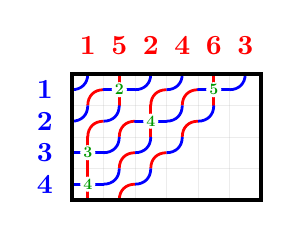
\begin{tikzpicture}[scale=0.4]
  \draw[lightgray, very thin, opacity=0.3] (0,2) -- (6,2);
  \draw[lightgray, very thin, opacity=0.3] (0,3) -- (6,3);
  \draw[lightgray, very thin, opacity=0.3] (0,4) -- (6,4);
  \draw[lightgray, very thin, opacity=0.3] (0,5) -- (6,5);
  \draw[lightgray, very thin, opacity=0.3] (0,6) -- (6,6);
  \draw[lightgray, very thin, opacity=0.3] (0,2) -- (0,6);
  \draw[lightgray, very thin, opacity=0.3] (1,2) -- (1,6);
  \draw[lightgray, very thin, opacity=0.3] (2,2) -- (2,6);
  \draw[lightgray, very thin, opacity=0.3] (3,2) -- (3,6);
  \draw[lightgray, very thin, opacity=0.3] (4,2) -- (4,6);
  \draw[lightgray, very thin, opacity=0.3] (5,2) -- (5,6);
  \draw[lightgray, very thin, opacity=0.3] (6,2) -- (6,6);
  \draw[blue, line width=1.0pt] (0,5.5) .. controls (0.3,5.5) and (0.5,5.7) .. (0.5,6);
  \draw[red, line width=1.0pt] (0.5,5) .. controls (0.5,5.3) and (0.7,5.5) .. (1,5.5);
  \draw[blue, line width=1.0pt, line cap=round] (1,5.5) -- (2,5.5);
  \draw[red, line width=1.0pt, line cap=round] (1.5,5) -- (1.5,6);
  \draw[blue, line width=1.0pt] (2,5.5) .. controls (2.3,5.5) and (2.5,5.7) .. (2.5,6);
  \draw[red, line width=1.0pt] (2.5,5) .. controls (2.5,5.3) and (2.7,5.5) .. (3,5.5);
  \draw[blue, line width=1.0pt] (3,5.5) .. controls (3.3,5.5) and (3.5,5.7) .. (3.5,6);
  \draw[red, line width=1.0pt] (3.5,5) .. controls (3.5,5.3) and (3.7,5.5) .. (4,5.5);
  \draw[blue, line width=1.0pt, line cap=round] (4,5.5) -- (5,5.5);
  \draw[red, line width=1.0pt, line cap=round] (4.5,5) -- (4.5,6);
  \draw[blue, line width=1.0pt] (5,5.5) .. controls (5.3,5.5) and (5.5,5.7) .. (5.5,6);
  \draw[blue, line width=1.0pt] (0,4.5) .. controls (0.3,4.5) and (0.5,4.7) .. (0.5,5);
  \draw[red, line width=1.0pt] (0.5,4) .. controls (0.5,4.3) and (0.7,4.5) .. (1,4.5);
  \draw[blue, line width=1.0pt] (1,4.5) .. controls (1.3,4.5) and (1.5,4.7) .. (1.5,5);
  \draw[red, line width=1.0pt] (1.5,4) .. controls (1.5,4.3) and (1.7,4.5) .. (2,4.5);
  \draw[blue, line width=1.0pt, line cap=round] (2,4.5) -- (3,4.5);
  \draw[red, line width=1.0pt, line cap=round] (2.5,4) -- (2.5,5);
  \draw[blue, line width=1.0pt] (3,4.5) .. controls (3.3,4.5) and (3.5,4.7) .. (3.5,5);
  \draw[red, line width=1.0pt] (3.5,4) .. controls (3.5,4.3) and (3.7,4.5) .. (4,4.5);
  \draw[blue, line width=1.0pt] (4,4.5) .. controls (4.3,4.5) and (4.5,4.7) .. (4.5,5);
  \draw[blue, line width=1.0pt, line cap=round] (0,3.5) -- (1,3.5);
  \draw[red, line width=1.0pt, line cap=round] (0.5,3) -- (0.5,4);
  \draw[blue, line width=1.0pt] (1,3.5) .. controls (1.3,3.5) and (1.5,3.7) .. (1.5,4);
  \draw[red, line width=1.0pt] (1.5,3) .. controls (1.5,3.3) and (1.7,3.5) .. (2,3.5);
  \draw[blue, line width=1.0pt] (2,3.5) .. controls (2.3,3.5) and (2.5,3.7) .. (2.5,4);
  \draw[red, line width=1.0pt] (2.5,3) .. controls (2.5,3.3) and (2.7,3.5) .. (3,3.5);
  \draw[blue, line width=1.0pt] (3,3.5) .. controls (3.3,3.5) and (3.5,3.7) .. (3.5,4);
  \draw[blue, line width=1.0pt, line cap=round] (0,2.5) -- (1,2.5);
  \draw[red, line width=1.0pt, line cap=round] (0.5,2) -- (0.5,3);
  \draw[blue, line width=1.0pt] (1,2.5) .. controls (1.3,2.5) and (1.5,2.7) .. (1.5,3);
  \draw[red, line width=1.0pt] (1.5,2) .. controls (1.5,2.3) and (1.7,2.5) .. (2,2.5);
  \draw[blue, line width=1.0pt] (2,2.5) .. controls (2.3,2.5) and (2.5,2.7) .. (2.5,3);
  \node[font=\Large\bfseries, text=green!60!black, fill=white, inner sep=0.5pt, circle, transform shape] at (1.5,5.5) {2};
  \node[font=\Large\bfseries, text=green!60!black, fill=white, inner sep=0.5pt, circle, transform shape] at (4.5,5.5) {5};
  \node[font=\Large\bfseries, text=green!60!black, fill=white, inner sep=0.5pt, circle, transform shape] at (0.5,3.5) {3};
  \node[font=\Large\bfseries, text=green!60!black, fill=white, inner sep=0.5pt, circle, transform shape] at (2.5,4.5) {4};
  \node[font=\Large\bfseries, text=green!60!black, fill=white, inner sep=0.5pt, circle, transform shape] at (0.5,2.5) {4};
  \node[font=\bfseries, text=red, anchor=south] at (0.5,6.3) {1};
  \node[font=\bfseries, text=red, anchor=south] at (1.5,6.3) {5};
  \node[font=\bfseries, text=red, anchor=south] at (2.5,6.3) {2};
  \node[font=\bfseries, text=red, anchor=south] at (3.5,6.3) {4};
  \node[font=\bfseries, text=red, anchor=south] at (4.5,6.3) {6};
  \node[font=\bfseries, text=red, anchor=south] at (5.5,6.3) {3};
  \node[font=\bfseries, text=blue, anchor=east] at (-0.3,5.5) {1};
  \node[font=\bfseries, text=blue, anchor=east] at (-0.3,4.5) {2};
  \node[font=\bfseries, text=blue, anchor=east] at (-0.3,3.5) {3};
  \node[font=\bfseries, text=blue, anchor=east] at (-0.3,2.5) {4};
  \draw[black, line width=1.2000000000000002pt] (0,2) rectangle (6,6);
\end{tikzpicture}}}
  +
  \vcenter{\hbox{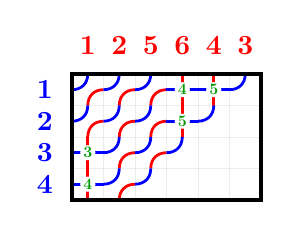
\begin{tikzpicture}[scale=0.4]
  \draw[lightgray, very thin, opacity=0.3] (0,2) -- (6,2);
  \draw[lightgray, very thin, opacity=0.3] (0,3) -- (6,3);
  \draw[lightgray, very thin, opacity=0.3] (0,4) -- (6,4);
  \draw[lightgray, very thin, opacity=0.3] (0,5) -- (6,5);
  \draw[lightgray, very thin, opacity=0.3] (0,6) -- (6,6);
  \draw[lightgray, very thin, opacity=0.3] (0,2) -- (0,6);
  \draw[lightgray, very thin, opacity=0.3] (1,2) -- (1,6);
  \draw[lightgray, very thin, opacity=0.3] (2,2) -- (2,6);
  \draw[lightgray, very thin, opacity=0.3] (3,2) -- (3,6);
  \draw[lightgray, very thin, opacity=0.3] (4,2) -- (4,6);
  \draw[lightgray, very thin, opacity=0.3] (5,2) -- (5,6);
  \draw[lightgray, very thin, opacity=0.3] (6,2) -- (6,6);
  \draw[blue, line width=1.0pt] (0,5.5) .. controls (0.3,5.5) and (0.5,5.7) .. (0.5,6);
  \draw[red, line width=1.0pt] (0.5,5) .. controls (0.5,5.3) and (0.7,5.5) .. (1,5.5);
  \draw[blue, line width=1.0pt] (1,5.5) .. controls (1.3,5.5) and (1.5,5.7) .. (1.5,6);
  \draw[red, line width=1.0pt] (1.5,5) .. controls (1.5,5.3) and (1.7,5.5) .. (2,5.5);
  \draw[blue, line width=1.0pt] (2,5.5) .. controls (2.3,5.5) and (2.5,5.7) .. (2.5,6);
  \draw[red, line width=1.0pt] (2.5,5) .. controls (2.5,5.3) and (2.7,5.5) .. (3,5.5);
  \draw[blue, line width=1.0pt, line cap=round] (3,5.5) -- (4,5.5);
  \draw[red, line width=1.0pt, line cap=round] (3.5,5) -- (3.5,6);
  \draw[blue, line width=1.0pt, line cap=round] (4,5.5) -- (5,5.5);
  \draw[red, line width=1.0pt, line cap=round] (4.5,5) -- (4.5,6);
  \draw[blue, line width=1.0pt] (5,5.5) .. controls (5.3,5.5) and (5.5,5.7) .. (5.5,6);
  \draw[blue, line width=1.0pt] (0,4.5) .. controls (0.3,4.5) and (0.5,4.7) .. (0.5,5);
  \draw[red, line width=1.0pt] (0.5,4) .. controls (0.5,4.3) and (0.7,4.5) .. (1,4.5);
  \draw[blue, line width=1.0pt] (1,4.5) .. controls (1.3,4.5) and (1.5,4.7) .. (1.5,5);
  \draw[red, line width=1.0pt] (1.5,4) .. controls (1.5,4.3) and (1.7,4.5) .. (2,4.5);
  \draw[blue, line width=1.0pt] (2,4.5) .. controls (2.3,4.5) and (2.5,4.7) .. (2.5,5);
  \draw[red, line width=1.0pt] (2.5,4) .. controls (2.5,4.3) and (2.7,4.5) .. (3,4.5);
  \draw[blue, line width=1.0pt, line cap=round] (3,4.5) -- (4,4.5);
  \draw[red, line width=1.0pt, line cap=round] (3.5,4) -- (3.5,5);
  \draw[blue, line width=1.0pt] (4,4.5) .. controls (4.3,4.5) and (4.5,4.7) .. (4.5,5);
  \draw[blue, line width=1.0pt, line cap=round] (0,3.5) -- (1,3.5);
  \draw[red, line width=1.0pt, line cap=round] (0.5,3) -- (0.5,4);
  \draw[blue, line width=1.0pt] (1,3.5) .. controls (1.3,3.5) and (1.5,3.7) .. (1.5,4);
  \draw[red, line width=1.0pt] (1.5,3) .. controls (1.5,3.3) and (1.7,3.5) .. (2,3.5);
  \draw[blue, line width=1.0pt] (2,3.5) .. controls (2.3,3.5) and (2.5,3.7) .. (2.5,4);
  \draw[red, line width=1.0pt] (2.5,3) .. controls (2.5,3.3) and (2.7,3.5) .. (3,3.5);
  \draw[blue, line width=1.0pt] (3,3.5) .. controls (3.3,3.5) and (3.5,3.7) .. (3.5,4);
  \draw[blue, line width=1.0pt, line cap=round] (0,2.5) -- (1,2.5);
  \draw[red, line width=1.0pt, line cap=round] (0.5,2) -- (0.5,3);
  \draw[blue, line width=1.0pt] (1,2.5) .. controls (1.3,2.5) and (1.5,2.7) .. (1.5,3);
  \draw[red, line width=1.0pt] (1.5,2) .. controls (1.5,2.3) and (1.7,2.5) .. (2,2.5);
  \draw[blue, line width=1.0pt] (2,2.5) .. controls (2.3,2.5) and (2.5,2.7) .. (2.5,3);
  \node[font=\Large\bfseries, text=green!60!black, fill=white, inner sep=0.5pt, circle, transform shape] at (3.5,4.5) {5};
  \node[font=\Large\bfseries, text=green!60!black, fill=white, inner sep=0.5pt, circle, transform shape] at (4.5,5.5) {5};
  \node[font=\Large\bfseries, text=green!60!black, fill=white, inner sep=0.5pt, circle, transform shape] at (0.5,3.5) {3};
  \node[font=\Large\bfseries, text=green!60!black, fill=white, inner sep=0.5pt, circle, transform shape] at (3.5,5.5) {4};
  \node[font=\Large\bfseries, text=green!60!black, fill=white, inner sep=0.5pt, circle, transform shape] at (0.5,2.5) {4};
  \node[font=\bfseries, text=red, anchor=south] at (0.5,6.3) {1};
  \node[font=\bfseries, text=red, anchor=south] at (1.5,6.3) {2};
  \node[font=\bfseries, text=red, anchor=south] at (2.5,6.3) {5};
  \node[font=\bfseries, text=red, anchor=south] at (3.5,6.3) {6};
  \node[font=\bfseries, text=red, anchor=south] at (4.5,6.3) {4};
  \node[font=\bfseries, text=red, anchor=south] at (5.5,6.3) {3};
  \node[font=\bfseries, text=blue, anchor=east] at (-0.3,5.5) {1};
  \node[font=\bfseries, text=blue, anchor=east] at (-0.3,4.5) {2};
  \node[font=\bfseries, text=blue, anchor=east] at (-0.3,3.5) {3};
  \node[font=\bfseries, text=blue, anchor=east] at (-0.3,2.5) {4};
  \draw[black, line width=1.2000000000000002pt] (0,2) rectangle (6,6);
\end{tikzpicture}}}
  \\[1em]
  + & 
  \vcenter{\hbox{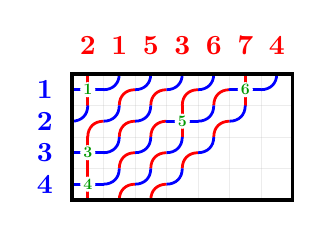
\begin{tikzpicture}[scale=0.4]
  \draw[lightgray, very thin, opacity=0.3] (0,3) -- (7,3);
  \draw[lightgray, very thin, opacity=0.3] (0,4) -- (7,4);
  \draw[lightgray, very thin, opacity=0.3] (0,5) -- (7,5);
  \draw[lightgray, very thin, opacity=0.3] (0,6) -- (7,6);
  \draw[lightgray, very thin, opacity=0.3] (0,7) -- (7,7);
  \draw[lightgray, very thin, opacity=0.3] (0,3) -- (0,7);
  \draw[lightgray, very thin, opacity=0.3] (1,3) -- (1,7);
  \draw[lightgray, very thin, opacity=0.3] (2,3) -- (2,7);
  \draw[lightgray, very thin, opacity=0.3] (3,3) -- (3,7);
  \draw[lightgray, very thin, opacity=0.3] (4,3) -- (4,7);
  \draw[lightgray, very thin, opacity=0.3] (5,3) -- (5,7);
  \draw[lightgray, very thin, opacity=0.3] (6,3) -- (6,7);
  \draw[lightgray, very thin, opacity=0.3] (7,3) -- (7,7);
  \draw[blue, line width=1.0pt, line cap=round] (0,6.5) -- (1,6.5);
  \draw[red, line width=1.0pt, line cap=round] (0.5,6) -- (0.5,7);
  \draw[blue, line width=1.0pt] (1,6.5) .. controls (1.3,6.5) and (1.5,6.7) .. (1.5,7);
  \draw[red, line width=1.0pt] (1.5,6) .. controls (1.5,6.3) and (1.7,6.5) .. (2,6.5);
  \draw[blue, line width=1.0pt] (2,6.5) .. controls (2.3,6.5) and (2.5,6.7) .. (2.5,7);
  \draw[red, line width=1.0pt] (2.5,6) .. controls (2.5,6.3) and (2.7,6.5) .. (3,6.5);
  \draw[blue, line width=1.0pt] (3,6.5) .. controls (3.3,6.5) and (3.5,6.7) .. (3.5,7);
  \draw[red, line width=1.0pt] (3.5,6) .. controls (3.5,6.3) and (3.7,6.5) .. (4,6.5);
  \draw[blue, line width=1.0pt] (4,6.5) .. controls (4.3,6.5) and (4.5,6.7) .. (4.5,7);
  \draw[red, line width=1.0pt] (4.5,6) .. controls (4.5,6.3) and (4.7,6.5) .. (5,6.5);
  \draw[blue, line width=1.0pt, line cap=round] (5,6.5) -- (6,6.5);
  \draw[red, line width=1.0pt, line cap=round] (5.5,6) -- (5.5,7);
  \draw[blue, line width=1.0pt] (6,6.5) .. controls (6.3,6.5) and (6.5,6.7) .. (6.5,7);
  \draw[blue, line width=1.0pt] (0,5.5) .. controls (0.3,5.5) and (0.5,5.7) .. (0.5,6);
  \draw[red, line width=1.0pt] (0.5,5) .. controls (0.5,5.3) and (0.7,5.5) .. (1,5.5);
  \draw[blue, line width=1.0pt] (1,5.5) .. controls (1.3,5.5) and (1.5,5.7) .. (1.5,6);
  \draw[red, line width=1.0pt] (1.5,5) .. controls (1.5,5.3) and (1.7,5.5) .. (2,5.5);
  \draw[blue, line width=1.0pt] (2,5.5) .. controls (2.3,5.5) and (2.5,5.7) .. (2.5,6);
  \draw[red, line width=1.0pt] (2.5,5) .. controls (2.5,5.3) and (2.7,5.5) .. (3,5.5);
  \draw[blue, line width=1.0pt, line cap=round] (3,5.5) -- (4,5.5);
  \draw[red, line width=1.0pt, line cap=round] (3.5,5) -- (3.5,6);
  \draw[blue, line width=1.0pt] (4,5.5) .. controls (4.3,5.5) and (4.5,5.7) .. (4.5,6);
  \draw[red, line width=1.0pt] (4.5,5) .. controls (4.5,5.3) and (4.7,5.5) .. (5,5.5);
  \draw[blue, line width=1.0pt] (5,5.5) .. controls (5.3,5.5) and (5.5,5.7) .. (5.5,6);
  \draw[blue, line width=1.0pt, line cap=round] (0,4.5) -- (1,4.5);
  \draw[red, line width=1.0pt, line cap=round] (0.5,4) -- (0.5,5);
  \draw[blue, line width=1.0pt] (1,4.5) .. controls (1.3,4.5) and (1.5,4.7) .. (1.5,5);
  \draw[red, line width=1.0pt] (1.5,4) .. controls (1.5,4.3) and (1.7,4.5) .. (2,4.5);
  \draw[blue, line width=1.0pt] (2,4.5) .. controls (2.3,4.5) and (2.5,4.7) .. (2.5,5);
  \draw[red, line width=1.0pt] (2.5,4) .. controls (2.5,4.3) and (2.7,4.5) .. (3,4.5);
  \draw[blue, line width=1.0pt] (3,4.5) .. controls (3.3,4.5) and (3.5,4.7) .. (3.5,5);
  \draw[red, line width=1.0pt] (3.5,4) .. controls (3.5,4.3) and (3.7,4.5) .. (4,4.5);
  \draw[blue, line width=1.0pt] (4,4.5) .. controls (4.3,4.5) and (4.5,4.7) .. (4.5,5);
  \draw[blue, line width=1.0pt, line cap=round] (0,3.5) -- (1,3.5);
  \draw[red, line width=1.0pt, line cap=round] (0.5,3) -- (0.5,4);
  \draw[blue, line width=1.0pt] (1,3.5) .. controls (1.3,3.5) and (1.5,3.7) .. (1.5,4);
  \draw[red, line width=1.0pt] (1.5,3) .. controls (1.5,3.3) and (1.7,3.5) .. (2,3.5);
  \draw[blue, line width=1.0pt] (2,3.5) .. controls (2.3,3.5) and (2.5,3.7) .. (2.5,4);
  \draw[red, line width=1.0pt] (2.5,3) .. controls (2.5,3.3) and (2.7,3.5) .. (3,3.5);
  \draw[blue, line width=1.0pt] (3,3.5) .. controls (3.3,3.5) and (3.5,3.7) .. (3.5,4);
  \node[font=\Large\bfseries, text=green!60!black, fill=white, inner sep=0.5pt, circle, transform shape] at (3.5,5.5) {5};
  \node[font=\Large\bfseries, text=green!60!black, fill=white, inner sep=0.5pt, circle, transform shape] at (0.5,4.5) {3};
  \node[font=\Large\bfseries, text=green!60!black, fill=white, inner sep=0.5pt, circle, transform shape] at (0.5,6.5) {1};
  \node[font=\Large\bfseries, text=green!60!black, fill=white, inner sep=0.5pt, circle, transform shape] at (5.5,6.5) {6};
  \node[font=\Large\bfseries, text=green!60!black, fill=white, inner sep=0.5pt, circle, transform shape] at (0.5,3.5) {4};
  \node[font=\bfseries, text=red, anchor=south] at (0.5,7.3) {2};
  \node[font=\bfseries, text=red, anchor=south] at (1.5,7.3) {1};
  \node[font=\bfseries, text=red, anchor=south] at (2.5,7.3) {5};
  \node[font=\bfseries, text=red, anchor=south] at (3.5,7.3) {3};
  \node[font=\bfseries, text=red, anchor=south] at (4.5,7.3) {6};
  \node[font=\bfseries, text=red, anchor=south] at (5.5,7.3) {7};
  \node[font=\bfseries, text=red, anchor=south] at (6.5,7.3) {4};
  \node[font=\bfseries, text=blue, anchor=east] at (-0.3,6.5) {1};
  \node[font=\bfseries, text=blue, anchor=east] at (-0.3,5.5) {2};
  \node[font=\bfseries, text=blue, anchor=east] at (-0.3,4.5) {3};
  \node[font=\bfseries, text=blue, anchor=east] at (-0.3,3.5) {4};
  \draw[black, line width=1.2000000000000002pt] (0,3) rectangle (7,7);
\end{tikzpicture}}}
  +
  \vcenter{\hbox{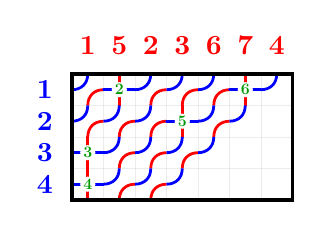
\begin{tikzpicture}[scale=0.4]
  \draw[lightgray, very thin, opacity=0.3] (0,3) -- (7,3);
  \draw[lightgray, very thin, opacity=0.3] (0,4) -- (7,4);
  \draw[lightgray, very thin, opacity=0.3] (0,5) -- (7,5);
  \draw[lightgray, very thin, opacity=0.3] (0,6) -- (7,6);
  \draw[lightgray, very thin, opacity=0.3] (0,7) -- (7,7);
  \draw[lightgray, very thin, opacity=0.3] (0,3) -- (0,7);
  \draw[lightgray, very thin, opacity=0.3] (1,3) -- (1,7);
  \draw[lightgray, very thin, opacity=0.3] (2,3) -- (2,7);
  \draw[lightgray, very thin, opacity=0.3] (3,3) -- (3,7);
  \draw[lightgray, very thin, opacity=0.3] (4,3) -- (4,7);
  \draw[lightgray, very thin, opacity=0.3] (5,3) -- (5,7);
  \draw[lightgray, very thin, opacity=0.3] (6,3) -- (6,7);
  \draw[lightgray, very thin, opacity=0.3] (7,3) -- (7,7);
  \draw[blue, line width=1.0pt] (0,6.5) .. controls (0.3,6.5) and (0.5,6.7) .. (0.5,7);
  \draw[red, line width=1.0pt] (0.5,6) .. controls (0.5,6.3) and (0.7,6.5) .. (1,6.5);
  \draw[blue, line width=1.0pt, line cap=round] (1,6.5) -- (2,6.5);
  \draw[red, line width=1.0pt, line cap=round] (1.5,6) -- (1.5,7);
  \draw[blue, line width=1.0pt] (2,6.5) .. controls (2.3,6.5) and (2.5,6.7) .. (2.5,7);
  \draw[red, line width=1.0pt] (2.5,6) .. controls (2.5,6.3) and (2.7,6.5) .. (3,6.5);
  \draw[blue, line width=1.0pt] (3,6.5) .. controls (3.3,6.5) and (3.5,6.7) .. (3.5,7);
  \draw[red, line width=1.0pt] (3.5,6) .. controls (3.5,6.3) and (3.7,6.5) .. (4,6.5);
  \draw[blue, line width=1.0pt] (4,6.5) .. controls (4.3,6.5) and (4.5,6.7) .. (4.5,7);
  \draw[red, line width=1.0pt] (4.5,6) .. controls (4.5,6.3) and (4.7,6.5) .. (5,6.5);
  \draw[blue, line width=1.0pt, line cap=round] (5,6.5) -- (6,6.5);
  \draw[red, line width=1.0pt, line cap=round] (5.5,6) -- (5.5,7);
  \draw[blue, line width=1.0pt] (6,6.5) .. controls (6.3,6.5) and (6.5,6.7) .. (6.5,7);
  \draw[blue, line width=1.0pt] (0,5.5) .. controls (0.3,5.5) and (0.5,5.7) .. (0.5,6);
  \draw[red, line width=1.0pt] (0.5,5) .. controls (0.5,5.3) and (0.7,5.5) .. (1,5.5);
  \draw[blue, line width=1.0pt] (1,5.5) .. controls (1.3,5.5) and (1.5,5.7) .. (1.5,6);
  \draw[red, line width=1.0pt] (1.5,5) .. controls (1.5,5.3) and (1.7,5.5) .. (2,5.5);
  \draw[blue, line width=1.0pt] (2,5.5) .. controls (2.3,5.5) and (2.5,5.7) .. (2.5,6);
  \draw[red, line width=1.0pt] (2.5,5) .. controls (2.5,5.3) and (2.7,5.5) .. (3,5.5);
  \draw[blue, line width=1.0pt, line cap=round] (3,5.5) -- (4,5.5);
  \draw[red, line width=1.0pt, line cap=round] (3.5,5) -- (3.5,6);
  \draw[blue, line width=1.0pt] (4,5.5) .. controls (4.3,5.5) and (4.5,5.7) .. (4.5,6);
  \draw[red, line width=1.0pt] (4.5,5) .. controls (4.5,5.3) and (4.7,5.5) .. (5,5.5);
  \draw[blue, line width=1.0pt] (5,5.5) .. controls (5.3,5.5) and (5.5,5.7) .. (5.5,6);
  \draw[blue, line width=1.0pt, line cap=round] (0,4.5) -- (1,4.5);
  \draw[red, line width=1.0pt, line cap=round] (0.5,4) -- (0.5,5);
  \draw[blue, line width=1.0pt] (1,4.5) .. controls (1.3,4.5) and (1.5,4.7) .. (1.5,5);
  \draw[red, line width=1.0pt] (1.5,4) .. controls (1.5,4.3) and (1.7,4.5) .. (2,4.5);
  \draw[blue, line width=1.0pt] (2,4.5) .. controls (2.3,4.5) and (2.5,4.7) .. (2.5,5);
  \draw[red, line width=1.0pt] (2.5,4) .. controls (2.5,4.3) and (2.7,4.5) .. (3,4.5);
  \draw[blue, line width=1.0pt] (3,4.5) .. controls (3.3,4.5) and (3.5,4.7) .. (3.5,5);
  \draw[red, line width=1.0pt] (3.5,4) .. controls (3.5,4.3) and (3.7,4.5) .. (4,4.5);
  \draw[blue, line width=1.0pt] (4,4.5) .. controls (4.3,4.5) and (4.5,4.7) .. (4.5,5);
  \draw[blue, line width=1.0pt, line cap=round] (0,3.5) -- (1,3.5);
  \draw[red, line width=1.0pt, line cap=round] (0.5,3) -- (0.5,4);
  \draw[blue, line width=1.0pt] (1,3.5) .. controls (1.3,3.5) and (1.5,3.7) .. (1.5,4);
  \draw[red, line width=1.0pt] (1.5,3) .. controls (1.5,3.3) and (1.7,3.5) .. (2,3.5);
  \draw[blue, line width=1.0pt] (2,3.5) .. controls (2.3,3.5) and (2.5,3.7) .. (2.5,4);
  \draw[red, line width=1.0pt] (2.5,3) .. controls (2.5,3.3) and (2.7,3.5) .. (3,3.5);
  \draw[blue, line width=1.0pt] (3,3.5) .. controls (3.3,3.5) and (3.5,3.7) .. (3.5,4);
  \node[font=\Large\bfseries, text=green!60!black, fill=white, inner sep=0.5pt, circle, transform shape] at (3.5,5.5) {5};
  \node[font=\Large\bfseries, text=green!60!black, fill=white, inner sep=0.5pt, circle, transform shape] at (1.5,6.5) {2};
  \node[font=\Large\bfseries, text=green!60!black, fill=white, inner sep=0.5pt, circle, transform shape] at (0.5,4.5) {3};
  \node[font=\Large\bfseries, text=green!60!black, fill=white, inner sep=0.5pt, circle, transform shape] at (5.5,6.5) {6};
  \node[font=\Large\bfseries, text=green!60!black, fill=white, inner sep=0.5pt, circle, transform shape] at (0.5,3.5) {4};
  \node[font=\bfseries, text=red, anchor=south] at (0.5,7.3) {1};
  \node[font=\bfseries, text=red, anchor=south] at (1.5,7.3) {5};
  \node[font=\bfseries, text=red, anchor=south] at (2.5,7.3) {2};
  \node[font=\bfseries, text=red, anchor=south] at (3.5,7.3) {3};
  \node[font=\bfseries, text=red, anchor=south] at (4.5,7.3) {6};
  \node[font=\bfseries, text=red, anchor=south] at (5.5,7.3) {7};
  \node[font=\bfseries, text=red, anchor=south] at (6.5,7.3) {4};
  \node[font=\bfseries, text=blue, anchor=east] at (-0.3,6.5) {1};
  \node[font=\bfseries, text=blue, anchor=east] at (-0.3,5.5) {2};
  \node[font=\bfseries, text=blue, anchor=east] at (-0.3,4.5) {3};
  \node[font=\bfseries, text=blue, anchor=east] at (-0.3,3.5) {4};
  \draw[black, line width=1.2000000000000002pt] (0,3) rectangle (7,7);
\end{tikzpicture}}}
  +
  \vcenter{\hbox{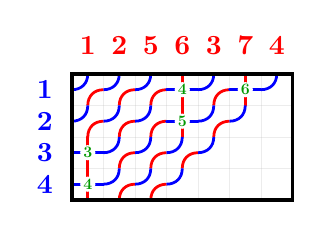
\begin{tikzpicture}[scale=0.4]
  \draw[lightgray, very thin, opacity=0.3] (0,3) -- (7,3);
  \draw[lightgray, very thin, opacity=0.3] (0,4) -- (7,4);
  \draw[lightgray, very thin, opacity=0.3] (0,5) -- (7,5);
  \draw[lightgray, very thin, opacity=0.3] (0,6) -- (7,6);
  \draw[lightgray, very thin, opacity=0.3] (0,7) -- (7,7);
  \draw[lightgray, very thin, opacity=0.3] (0,3) -- (0,7);
  \draw[lightgray, very thin, opacity=0.3] (1,3) -- (1,7);
  \draw[lightgray, very thin, opacity=0.3] (2,3) -- (2,7);
  \draw[lightgray, very thin, opacity=0.3] (3,3) -- (3,7);
  \draw[lightgray, very thin, opacity=0.3] (4,3) -- (4,7);
  \draw[lightgray, very thin, opacity=0.3] (5,3) -- (5,7);
  \draw[lightgray, very thin, opacity=0.3] (6,3) -- (6,7);
  \draw[lightgray, very thin, opacity=0.3] (7,3) -- (7,7);
  \draw[blue, line width=1.0pt] (0,6.5) .. controls (0.3,6.5) and (0.5,6.7) .. (0.5,7);
  \draw[red, line width=1.0pt] (0.5,6) .. controls (0.5,6.3) and (0.7,6.5) .. (1,6.5);
  \draw[blue, line width=1.0pt] (1,6.5) .. controls (1.3,6.5) and (1.5,6.7) .. (1.5,7);
  \draw[red, line width=1.0pt] (1.5,6) .. controls (1.5,6.3) and (1.7,6.5) .. (2,6.5);
  \draw[blue, line width=1.0pt] (2,6.5) .. controls (2.3,6.5) and (2.5,6.7) .. (2.5,7);
  \draw[red, line width=1.0pt] (2.5,6) .. controls (2.5,6.3) and (2.7,6.5) .. (3,6.5);
  \draw[blue, line width=1.0pt, line cap=round] (3,6.5) -- (4,6.5);
  \draw[red, line width=1.0pt, line cap=round] (3.5,6) -- (3.5,7);
  \draw[blue, line width=1.0pt] (4,6.5) .. controls (4.3,6.5) and (4.5,6.7) .. (4.5,7);
  \draw[red, line width=1.0pt] (4.5,6) .. controls (4.5,6.3) and (4.7,6.5) .. (5,6.5);
  \draw[blue, line width=1.0pt, line cap=round] (5,6.5) -- (6,6.5);
  \draw[red, line width=1.0pt, line cap=round] (5.5,6) -- (5.5,7);
  \draw[blue, line width=1.0pt] (6,6.5) .. controls (6.3,6.5) and (6.5,6.7) .. (6.5,7);
  \draw[blue, line width=1.0pt] (0,5.5) .. controls (0.3,5.5) and (0.5,5.7) .. (0.5,6);
  \draw[red, line width=1.0pt] (0.5,5) .. controls (0.5,5.3) and (0.7,5.5) .. (1,5.5);
  \draw[blue, line width=1.0pt] (1,5.5) .. controls (1.3,5.5) and (1.5,5.7) .. (1.5,6);
  \draw[red, line width=1.0pt] (1.5,5) .. controls (1.5,5.3) and (1.7,5.5) .. (2,5.5);
  \draw[blue, line width=1.0pt] (2,5.5) .. controls (2.3,5.5) and (2.5,5.7) .. (2.5,6);
  \draw[red, line width=1.0pt] (2.5,5) .. controls (2.5,5.3) and (2.7,5.5) .. (3,5.5);
  \draw[blue, line width=1.0pt, line cap=round] (3,5.5) -- (4,5.5);
  \draw[red, line width=1.0pt, line cap=round] (3.5,5) -- (3.5,6);
  \draw[blue, line width=1.0pt] (4,5.5) .. controls (4.3,5.5) and (4.5,5.7) .. (4.5,6);
  \draw[red, line width=1.0pt] (4.5,5) .. controls (4.5,5.3) and (4.7,5.5) .. (5,5.5);
  \draw[blue, line width=1.0pt] (5,5.5) .. controls (5.3,5.5) and (5.5,5.7) .. (5.5,6);
  \draw[blue, line width=1.0pt, line cap=round] (0,4.5) -- (1,4.5);
  \draw[red, line width=1.0pt, line cap=round] (0.5,4) -- (0.5,5);
  \draw[blue, line width=1.0pt] (1,4.5) .. controls (1.3,4.5) and (1.5,4.7) .. (1.5,5);
  \draw[red, line width=1.0pt] (1.5,4) .. controls (1.5,4.3) and (1.7,4.5) .. (2,4.5);
  \draw[blue, line width=1.0pt] (2,4.5) .. controls (2.3,4.5) and (2.5,4.7) .. (2.5,5);
  \draw[red, line width=1.0pt] (2.5,4) .. controls (2.5,4.3) and (2.7,4.5) .. (3,4.5);
  \draw[blue, line width=1.0pt] (3,4.5) .. controls (3.3,4.5) and (3.5,4.7) .. (3.5,5);
  \draw[red, line width=1.0pt] (3.5,4) .. controls (3.5,4.3) and (3.7,4.5) .. (4,4.5);
  \draw[blue, line width=1.0pt] (4,4.5) .. controls (4.3,4.5) and (4.5,4.7) .. (4.5,5);
  \draw[blue, line width=1.0pt, line cap=round] (0,3.5) -- (1,3.5);
  \draw[red, line width=1.0pt, line cap=round] (0.5,3) -- (0.5,4);
  \draw[blue, line width=1.0pt] (1,3.5) .. controls (1.3,3.5) and (1.5,3.7) .. (1.5,4);
  \draw[red, line width=1.0pt] (1.5,3) .. controls (1.5,3.3) and (1.7,3.5) .. (2,3.5);
  \draw[blue, line width=1.0pt] (2,3.5) .. controls (2.3,3.5) and (2.5,3.7) .. (2.5,4);
  \draw[red, line width=1.0pt] (2.5,3) .. controls (2.5,3.3) and (2.7,3.5) .. (3,3.5);
  \draw[blue, line width=1.0pt] (3,3.5) .. controls (3.3,3.5) and (3.5,3.7) .. (3.5,4);
  \node[font=\Large\bfseries, text=green!60!black, fill=white, inner sep=0.5pt, circle, transform shape] at (3.5,5.5) {5};
  \node[font=\Large\bfseries, text=green!60!black, fill=white, inner sep=0.5pt, circle, transform shape] at (0.5,4.5) {3};
  \node[font=\Large\bfseries, text=green!60!black, fill=white, inner sep=0.5pt, circle, transform shape] at (3.5,6.5) {4};
  \node[font=\Large\bfseries, text=green!60!black, fill=white, inner sep=0.5pt, circle, transform shape] at (5.5,6.5) {6};
  \node[font=\Large\bfseries, text=green!60!black, fill=white, inner sep=0.5pt, circle, transform shape] at (0.5,3.5) {4};
  \node[font=\bfseries, text=red, anchor=south] at (0.5,7.3) {1};
  \node[font=\bfseries, text=red, anchor=south] at (1.5,7.3) {2};
  \node[font=\bfseries, text=red, anchor=south] at (2.5,7.3) {5};
  \node[font=\bfseries, text=red, anchor=south] at (3.5,7.3) {6};
  \node[font=\bfseries, text=red, anchor=south] at (4.5,7.3) {3};
  \node[font=\bfseries, text=red, anchor=south] at (5.5,7.3) {7};
  \node[font=\bfseries, text=red, anchor=south] at (6.5,7.3) {4};
  \node[font=\bfseries, text=blue, anchor=east] at (-0.3,6.5) {1};
  \node[font=\bfseries, text=blue, anchor=east] at (-0.3,5.5) {2};
  \node[font=\bfseries, text=blue, anchor=east] at (-0.3,4.5) {3};
  \node[font=\bfseries, text=blue, anchor=east] at (-0.3,3.5) {4};
  \draw[black, line width=1.2000000000000002pt] (0,3) rectangle (7,7);
\end{tikzpicture}}}
\end{align*}


% To use this in a LaTeX document:
% \documentclass{article}
% \usepackage{amsmath}
% \usepackage{tikz}
% \begin{document}
% [paste the generated code here]
% \end{document}






\end{example}



\subsection{Preservation of the Assaf-Schilling Demazure crystal structure}

RC-graphs have a Demazure crystal structure defined by Assaf and Schilling in \cite{assaf2018demazure}. We may transport this structure to bounded RC graphs as  operators $e_i:\mathcal{RC}\to\mathcal{RC}\cup\{\emptyset\}$ and $f_i:\mathcal{RC}\to\mathcal{RC}\cup\{\emptyset\}$ by
$$e_i(R,n) = (e_i(R), n)$$
and
$$f_i(R, n)=(f_i(R), n)$$

\begin{lemma}
	Let $(R, n)$ be a bounded RC graph. If $f_i(R)\neq \emptyset$ and $\zeromap(R', n+1)=(R, n)$, then $f_i(R')\neq \emptyset$ and
	$$\zeromap(f_i(R'), n + 1)=(f_i(R), n)$$	
\end{lemma}

\begin{theorem}
	Let $(R, n)$ be a highest weight bounded RC graph and let $B(R, n)$ be the corresponding Demazure crystal. Let $B(R, n)^0$ be the subset of $B(R, n)$ such that the last row is empty. Then 
	$$\zeromap:B(R, n)^0\to \bigcup_{R'\in B(R,n)^0}B(\zeromap(R', n))$$ 
	is an isomorphism of crystal graphs.
\end{theorem}

An RC graph $R$ has a uniquely associated reduced word $\mathrm{word}(R)=(s_{i_1},\ldots,s_{i_N})$. Recall the Coxeter-Knuth relation $\sim_{\mathrm{CK}}$ defined by
$$j\ i\ k \sim_{\mathrm{CK}} j\ k\ i$$
and
$$k\ i\ j \sim_{\mathrm{CK}} i\ k\ j$$
if $i<j<k$, and
$$i\ i+1\ i \sim_{\mathrm{CK}} i+1\ i\ i+1$$
For an element $w\in S_\infty$, define $N(w)$ to be the minimal $N$ such that $w\in S_N$. For an RC graph $R$, define
$$\widetilde{\mathrm{eg}}(R) = (N(\wof{R}) - i_1, \ldots, N(\wof{R}) - i_N)$$
Via the Edelman-Greene insertion algorithm, we may define a pair
$$(P, Q)$$
of tableaux of the same shape such that the reading word of $P$ is CK-equivalent to $\widetilde{\mathrm{eg}}(R)$ and $Q$ has the same weight as $R$.

\begin{lemma}
	We have that
	$$R\mapsto Q$$
	 induces a morphism of crystal graphs into $B(\mathrm{shape}(Q))$. 
\end{lemma}

\begin{theorem}
	Let $R,R'$ be RC graphs. Then $\mathrm{hw}(R) = \mathrm{hw}(R')$ if and only if $\widetilde{\mathrm{eg}}(R) \sim_{\mathrm{CK}} \widetilde{\mathrm{eg}}(R')$.
\end{theorem}


\subsection{Crystal divided differences and the dominant Pieri formula}

Let $R$ be an RC graph and let $i>0$ be an integer. We define $\rcdd^iR$, an element of $\RC$, as follows. Define
$$\rcdd^iR=0$$
unless $s_i$ is a right descent of $\wof{R}$ and there exists $(i,j)\in R$ such that $\rtt_R(i, j) = (i, i+1)$. If these latter two conditions are satisfied, define 
$$R'=R\setminus \{(i, j)\}$$
where $\rtt_R(i,j) = (i, i+1)$. If $e_i(R')\neq \emptyset$, define $\rcdd^iR'=0$. Otherwise, define
$$\rcdd^iR = \sum_{p=0}^{\varphi_i(R')}f_i^pR'$$
\begin{lemma} \label{lemma:divdiffunique}
	Let $R$ be an RC graph and let $i>0$ be an integer. If $s_i$ is not a right descent of $\wof{R}$, then there is a unique $R'$ such that the coefficient of $R$ in $\rcdd^iR'$ is $1$, and for other $R'$ the coefficient is $0$.
\end{lemma}
\begin{proof}
	Suppose $s_i$ is not a right descent of $\wof{R}$. Assume without loss of generality that $e_iR = \emptyset$. If $(i+1, 1)\notin R$, then $(i,1)\notin R$ because $s_i$ is not a right descent of $\wof{R}$. In that case, let $R' = R\cup\{(i,1)\}$. Then 
	$$\rcdd^iR' = R + \text{other terms}$$ 
	If instead $(i+1, 1)\in R$, since $e_i(R)=\emptyset$ it follows that $(i, 1)\in R$, and if $j$ is the maximum value such that $(i+1,j')\in R$ for all $j'<j$, it follows that $(i,j')\in R$ for all $j'<j$. We must have that $(i,j+1)\notin R$, because $\rtt_R(i, j+1)=(i, i+1)$. Setting $R'=R\cup \{(i, j+1)\}$ gives us the result.
\end{proof}

\begin{theorem}
	Suppose $w\in S_\infty$ and $i >0$. If $i$ is not a right descent of $w$, then
	$$\rcdd^i\mathcal{S}_w(n) = 0$$
	Otherwise,
	$$\rcdd^i\mathcal{S}_w(n) = \mathcal{S}_{ws_i}(n)$$
\end{theorem}
\begin{proof}
	The result is trivial if $i$ is not a right descent of $w$. Suppose $i$ is a right descent of $w$. By Lemma \ref{lemma:divdiffunique}, for each RC graph $R$ such that $\wof{R} = ws_i$, there is a unique RC graph $R'$ such that the coefficient of $R$ in $\rcdd^iR'$ is $1$. Since $\wof{R'} = w$, the result follows.
\end{proof}

\begin{definition}
For a permutation $w$, define the \emph{principal RC graph} $R^0(w)$ of $w$ to be
$$R^0(w) = \{(i,j)\mid 1\leq j\leq \code^*_i(w)\}$$
\end{definition}

\begin{theorem}
Let $R$ be an RC graph and let $w=\wof{R}$. Then
$$\rcdd^wR = \delta_{R,R^0(w)}\emptyset$$
\end{theorem}

\begin{theorem}
For all $i>0$ we have
$$\rcdd^i\rcdd^i = 0$$
and
$$\rcdd^i\rcdd^{i+1}\rcdd^i = \rcdd^{i+1}\rcdd^i\rcdd^{i+1}$$
\end{theorem}
\begin{proof}
In order for $\rcdd^i\rcdd^{i+1}\rcdd^iR$ to be nonzero, first of all there must be an $(i,j)\in R$ such that $\rtt_R(i,j)=(i,i+1)$. Also, $R_1 = R\setminus\{(i,j)\}$ must satisfy $e_iR_1=\emptyset$, and there must be a $p$ such that if we define
$$R_1^{(p)}=f_i^pR_1$$
then there is an $(i+1,k)\in R_1^{(p)}$ such that $\rtt_{R_1^{(p)}}(i+1,k)=(i+1,i+2)$. By construction, in fact we must have that this is true for all $p$ for which $R_1^{(p)}\neq \emptyset$. Next, define
$$R_{12}^{(p)} = R_1^{(p)}\setminus\{(i+1,k)\}$$
Then we must have that $e_{i+1}R_{12}^{(p)}=\emptyset$, and if we define
$$R_{12}^{(p,q)} = f_{i+1}^qR_{12}^{(p)}$$
All such elements will have an $(i, m)\in R_{12}^{(p,q)}$ such that $\rtt_{R_{12}^{(p,q)}}(i,m)=(i,i+1)$. Then defining
$$R_{121}^{(p,q)} = R_{12}^{(p,q)}\setminus\{(i,m)\}$$
we must have that $e_iR_{121}^{(p,q)}=\emptyset$. Then if we define
$$R_{121}^{(p,q,r)} = f_i^rR_{121}^{(p,q)}$$
we have that
$$\rcdd^i\rcdd^{i+1}\rcdd^iR = \sum_{p,q,r} R_{121}^{(p,q,r)}$$
More concisely,
$$R_{121}^{(p,q,r)} = f_i^r( (f_{i+1}^q (f_i^p (R\setminus\{(i,j)\}))\setminus\{(i+1,k)\})\setminus\{ (i,m)\})$$
Similarly,
$$R_{212}^{(p,q,r)} = f_{i+1}^r( (f_{i}^q (f_{i+1}^p (R\setminus\{(i+1,k)\}))\setminus\{(i,m)\})\setminus\{ (i+1,j+1)\})$$
\end{proof}
%\begin{definition}
%	For integers $p,q$, define a permutation
%	$$d[p,q] = s_ps_{p+1}\cdots s_{p+q-1}$$
%	For a bounded RC graph $(R,n)$ and an integer $1\leq i\leq n$ such that row $i$ is empty, define $Z_{(i)}(R, n)$ as follows. Let 
%	$$R^-=\{(a,b)\mid (a,b)\in R\mbox{ and }a<i\}$$
%	and
%	$$R^+=\{(a,b)\mid (a,b)\in R\mbox{ and }a>i\}$$
%	Then define $R'$ to be the unique RC graph such that
%	$$(R', i-1) = Z^{n-i+1}(R^-, n)$$ 
%	Finally, define
%	$$R_{(i)}=R'\cup\trm(R^+)$$
%	and
%	$$Z_{(i)}(R, n) = (R_{(i)}, n-1)$$
%	
%	Let $\mu$ be a dominant permutation, let $w$ be an arbitrary permutation, and let $R$ be an RC graph. We define an integer $\delta_\mu^w(R)\in\{0,1\}$ by the following algorithm. Set $R_0=R$ and begin iterating, setting $i=1$. If $\code^*_i(\mu)>\code^*_i(w)$, terminate and set $\delta_\mu^w(R)=0$. Otherwise, define
%	$$R' = \partial^{d[\code_i^*(\mu)+1,\code^*_i(w)-\code^*_i(\mu)]}(R_{i-1})$$
%	If row $\code_i^*(\mu)+1$ is not empty in $R'$, terminate and set $\delta_\mu^w(R) = 0$. Otherwise, let 
%	$$R_i = Z_{(\code_i^*(\mu)+1)}(R', n - i + 1)$$
%	 Let $m$ be the length of $\code^*(\mu)$, and proceed as $i$ ranges from $1$ to $m$. After this procedure, we end with the RC graph $R_m$. If there is an index past $m$ such that $\code^*(w)$ is nonzero, proceed incrementally for each $i > m$ by applying
%	 $$R_i = \partial^{d[i+1-m, \code^*_i(w)]}(R_{i-1})$$
%	 then define
%	 $$\delta_\mu^w(R) = 1$$
%	 if $R_N=(\emptyset, 0)$ for sufficiently large $N$.
%\end{definition}

\begin{definition}
	Let $(R, n)$ be a bounded RC graph. We define a $\{0,1\}$-valued function $\delta_\mu^w(R, n)$ for a dominant permutation $\mu$ and an arbitrary permutation $w$ via the following construction. For integers $p, q$, let $d[p, q] = s_p s_{p+1} \cdots s_{p+q-1}$ be a product of simple reflections.
		
	Let $m$ be the length of $\code^*(\mu)$. Initialize $(R_0, n_0) = (R, n)$. For each $i$ from $1$ to $m$:
	\begin{enumerate}
		\item If $\code^*_i(\mu) > \code^*_i(w)$, terminate and set $\delta_\mu^w(R, n) = 0$.
		\item Otherwise, let $k = \code^*_i(w) - \code^*_i(\mu)$ and apply the crystal divided difference operator:
		\[
		R' = \rcdd^{d[\code_i^*(\mu)+1, \, k]}(R_{i-1})
		\]
		\item If row $\code_i^*(\mu)+1$ is not empty in $R'$, terminate and set $\delta_\mu^w(R, n) = 0$.
		\item If the row is empty, define the next state:
		\[
		(R_i, n_i) = Z_{(\code_i^*(\mu)+1)}(R', n_{i-1})
		\]
	\end{enumerate}
	
	If the loop completes, for any remaining indices $i > m$ where $\code^*_i(w) > 0$, incrementally update the graph:
	\[
	R_i = \rcdd^{d[i+1-m, \, \code^*_i(w)]}(R_{i-1})
	\]
	Finally, define $\delta_\mu^w(R, n) = 1$ if $(R_N, n_N) = (\emptyset, 0)$ for sufficiently large $N$, and $\delta_\mu^w(R, n) = 0$ otherwise.
\end{definition}

\begin{theorem}
	Let $\mu$ be a dominant permutation and let $v,w$ be permutations such that $\ell(\mu) + \ell(v)=\ell(w)$. Then
	$$c_{\mu,v}^w=\sum_{\wof{R}=v}\delta_\mu^w(R)$$
\end{theorem}

\section{Quantum rules}

\begin{theorem}
	We have
	$$\sch_u^q(x;y)E_{p,n_k}^q(x;z) = \sum_{{(d_1,\ldots,d_n)\in \scriptstyle{\mathrm{Pie}_{k, p}(u)}}} \sum_{u\tau_{\mathbf{d}}\tom{k} w\phi_{\mathbf{d}}} E_{p-F_{n_k}(u,w),n_k-F_{n_k}(u,w)}(y_{P_{n_k}(u,w)};z)q^{d_1}\cdots q^{d_n}\sch_w^q(x;y)$$
\end{theorem}


\bibliographystyle{acm}
\bibliography{formschub}


\end{document}